\chapter{راهنمای استفاده از کلاس \lr{yazd-thesis}}
\section{مقدمه}
حروف‌چینی پایان‌نامه یا رساله یکی از موارد پرکاربرد استفاده از زی‌پرشین است. از طرفی، یک  پایان‌نامه یا رساله،  احتیاج به تنظیمات زیادی از نظر صفحه‌آرایی  دارد که ممکن است برای
یک کاربر مبتدی، مشکل باشد. به همین خاطر، برای راحتی کار کاربر، کلاس حاضر با نام 
 \LRE{\verb!yazd-thesis!}
 برای حروف‌چینی پروژه‌ها، پایان‌نامه‌ها و رساله‌های دانشگاه یزد با استفاده از نرم‌افزار زی‌پرشین،  آماده شده است. این فایل به 
گونه‌ای طراحی شده است که کلیه خواسته‌های مورد نیاز  مدیریت تحصیلات تکمیلی دانشگاه یزد را برآورده می‌کند. همچنین حروف‌چینی بسیاری
از قسمت‌های آن، به طور خودکار انجام می‌شود.

کلیه فایل‌های لازم برای حروف‌چینی با کلاس گفته شده، داخل پوشه‌ای به نام
 \LRE{\verb!yazd-thesis!}
  قرار داده شده است. توجه داشته باشید که برای استفاده از این کلاس باید فونت‌های \lr{Yas}، \lr{Times New Roman}، 
  \lr{B Nazanin}  و \lr{Titr} روی کامپیوتر شما نصب باشد. این فونت‌ها در بین فونت‌های مشخص شده جهت نصب وجود دارد، ولی با توجه به این که
  ممکن است نصب \TeX{}Live از طریق دیگری انجام شده باشد، فونت‌های لازم در مسیر Fonts قرار گرفته است. می‌توانید این فونت‌ها را روی سیستم‌عامل
  خود نصب نمایید. تاکید می‌شود، در صورت نصب فونت، اگر با پیام وجود فونت روی کامپیوتر خود مواجه شدید، گزینه رونویسی فونت را انتخاب کنید تا از
  استفاده از نگارش مناسب فونت‌ها اطمینان حاصل نمایید.
 
\section{این همه فایل؟!}\label{sec2}
از آنجایی که یک پایان‌نامه یا رساله، یک نوشته بلند محسوب می‌شود، لذا اگر همه تنظیمات و مطالب پایان‌نامه را داخل یک فایل قرار بدهیم، باعث شلوغی
و سردرگمی می‌شود. به همین خاطر، قسمت‌های مختلف پایان‌نامه یا رساله  داخل فایل‌های جداگانه قرار گرفته است. مثلاً تنظیمات  کلاس داخل فایل
\LRE{\verb!yazd-thesis.cls!}، 
قسمت مشخصات فارسی پایان‌نامه داخل 
\LRE{\verb!fainfo.tex!}،
مطالب فصل اول، داخل 
\verb!chapter1!
و ... قرار داده شده است. نکته مهمی که در اینجا وجود دارد این است که از بین این  فایل‌ها، فقط فایل 
\LRE{\verb!yazd-thesis-template.tex!}
قابل اجرا است. یعنی بعد از تغییر فایل‌های دیگر، برای دیدن نتیجه تغییرات، باید این فایل را اجرا کرد. بقیه فایل‌ها به این فایل، کمک می‌کنند تا بتوانیم خروجی کار را ببینیم. اگر به فایل 
\LRE{\verb!yazd-thesis-template.tex!}
دقت کنید، متوجه می‌شوید که قسمت‌های مختلف پایان‌نامه، توسط دستورهایی مانند 
\verb!input!
و
\verb!include!
به فایل اصلی، یعنی 
\LRE{\verb!yazd-thesis-template.tex!}
معرفی شده‌اند. بنابراین، فایلی که همیشه با آن سروکار داریم، فایل 
\LRE{\verb!yazd-thesis-template.tex!}
است.
در این فایل، فرض شده است که پایان‌نامه یا رساله، از ۳ فصل و یک پیوست، تشکیل شده است. با این حال، اگر
  پایان‌نامه یا رساله، بیشتر از ۳ فصل و یک پیوست است، باید خودتان فصل‌های بیشتر را به این فایل، اضافه کنید. این کار، بسیار ساده است. فرض کنید بخواهید یک فصل دیگر هم به پایان‌نامه، اضافه کنید. برای این کار، کافی است یک فایل با نام 
\verb!chapter4!
و با پسوند 
\verb!.tex!
بسازید و آن را داخل پوشه 
\LRE{\verb!yazd-thesis!}
قرار دهید و سپس این فایل را با دستور 
\verb!\chapter[برخی نکات مفید]{ برخی نکات مفید ( اضافه کردن عنوان برای بیش از یک خط شدن)}
\twocolumnfootnotes
\section{فرایند تصویب پیشنهادیۀ پارسای تحصیلات تکمیلی}
در این بخش، فرآیند تصویب پیشنهادیۀ پایان‌نامه/رساله آورده شده است. 
دستورالعمل کامل مراحل تصویب و ثبت پیشنهادیۀ پایان‌نامه/ رساله دانشجویان تحصیلات تکمیلی در پیوست~\ref{ch:proposal}
آمده است.

لطفا برای مشاهده آخرین تغییرات به وبسایت تحصیلات تکمیلی دانشگاه به آدرس

\centerline{\url{https://yazd.ac.ir/offices/educational/deputy/graduate/home/rules}}

مراجعه نمایید.

\centerline{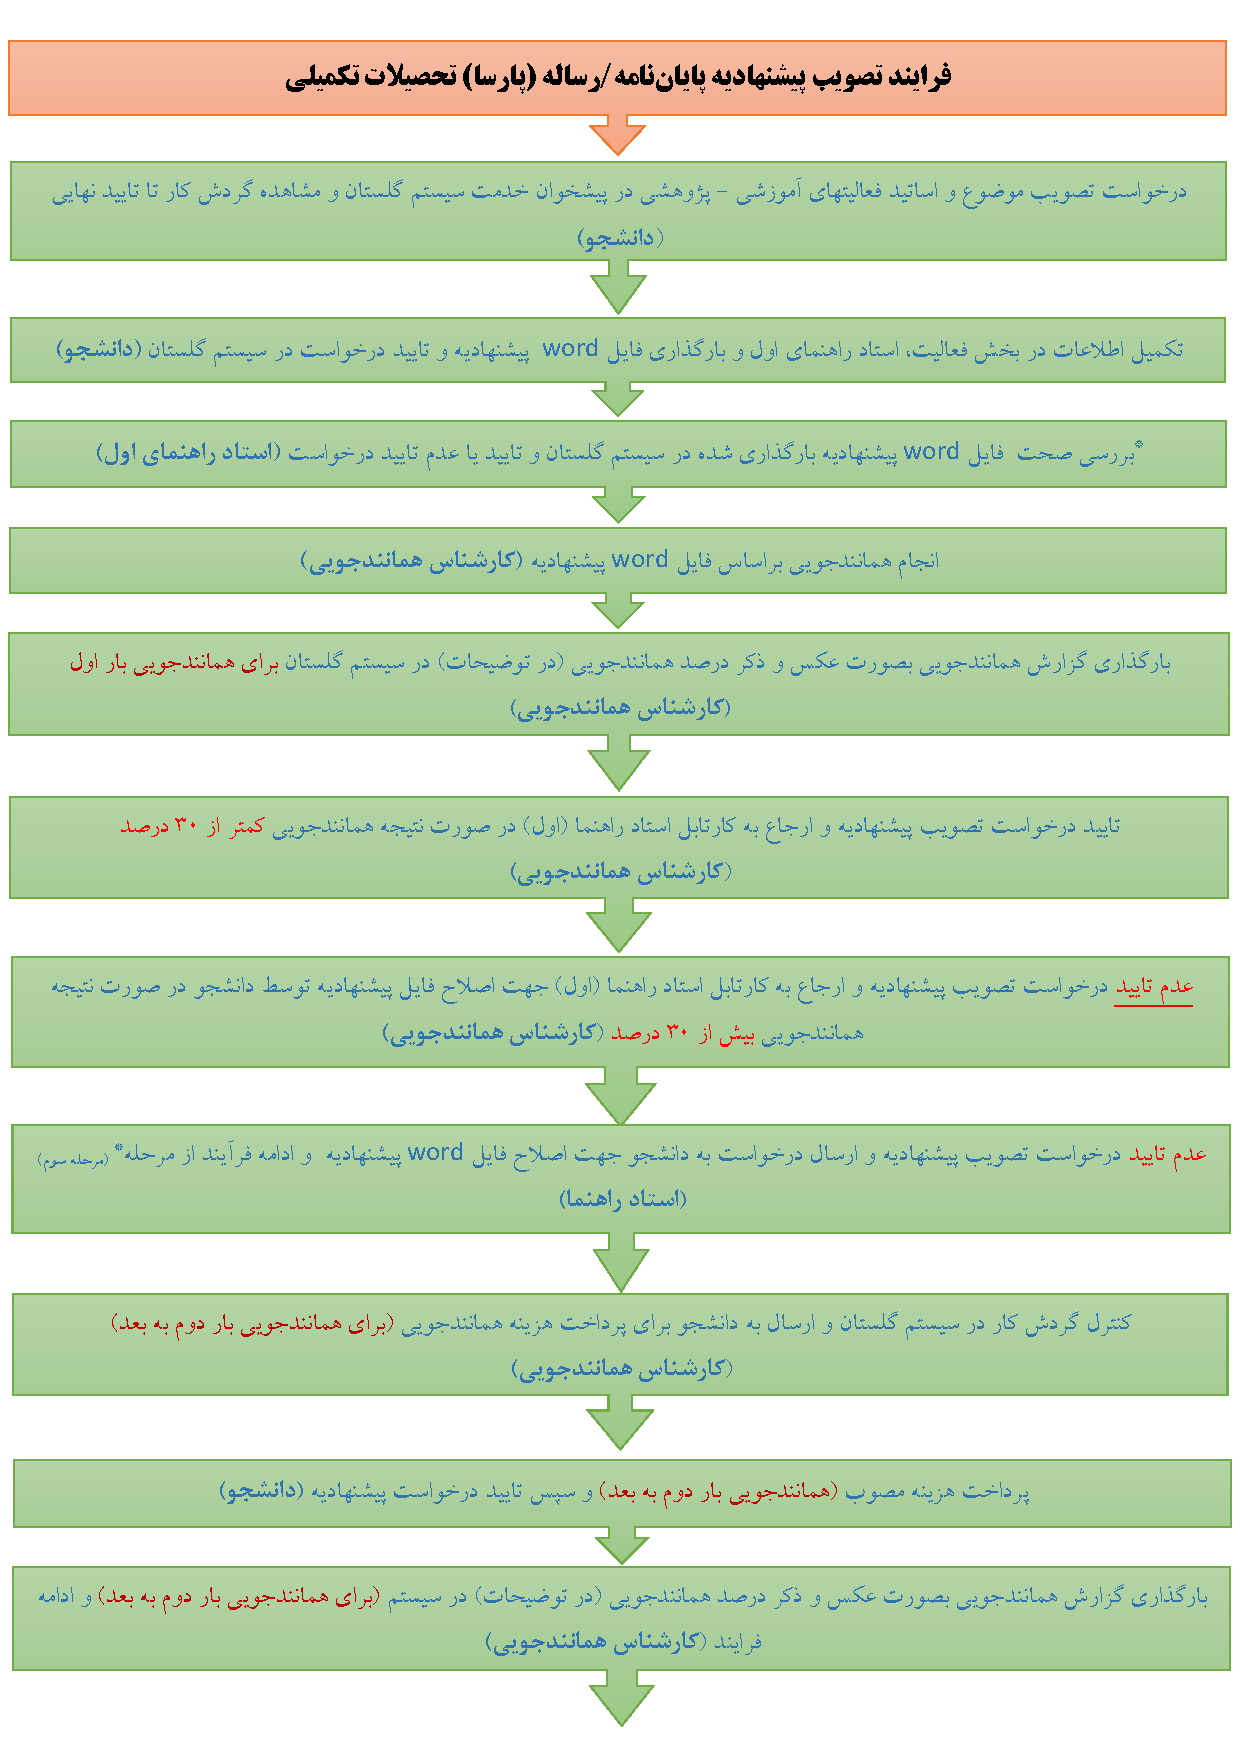
\includegraphics[width=0.9\textwidth]{Proposal-chart_Part1}}

\centerline{\includegraphics[width=\textwidth]{Proposal-chart_Part2}}

\section{دستورالعمل نحوه برگزاری جلسات دفاع }
\subsection{هدف }
هدف از تدوین این دستورالعمل ایجاد نظم و ترتیب بیشتر و شفاف‌سازی چگونگی برگزاری جلسات دفاع پایان‌نامه 
کارشناسی ارشد و رساله دکتری  و یادآوری نکات مهم برای برگزاری جلسه مطابق مقررات و شیوه‌نامه‌های تحصیلات تکمیلی‌است 
که بر اساس صورتجلسه شورای تحصیلات تکمیلی دانشگاه مورخ 17/2/1397 توسط نماینده تحصیلات تکمیلی (ناظر جلسه دفاعیه) 
دانشگاه مدیریت می‌گردد. 

\subsection{الف) فرآیند دفاع از پایان‌نامه / رساله }

\begin{enumerate}
\item  دانشجو: درخواست دفاع در پیشخوان خدمت

دانشجو در این قسمت ضمن درخواست دفاع‏، تاریخ و محل پیشنهادی دفاع از پایان‌نامه / رساله را بر اساس هماهنگی به عمل آمده
 با استادان راهنما / مشاور و پس از تایید اولیه رئیس بخش/ مدیرگروه ثبت می‌نماید. 
برای این منظور لازم است: 

*‌ دانشجو ظرف 48 ساعت، پایان‌نامه / رساله خود را همراه با مقالات مستخرج و تأییدیه‌های مجلات برای طرح در شورا به
 رئیس بخش / مدیرگروه تحویل و پس از تصویب جزئیات دفاع در شورا، فایل پایان‌نامه / رساله تصحیح شده نهایی و دستاوردهای
 مستخرج از آن را برای كارشناس تحصیلات تكمیلی ارسال کرده و فرآیند دفاع را تا مرحله تأیید معاون دانشكده / مدیرگروه مستقل پیگیری می‌نماید. 
 
*‌ برای دانشجویان دکتری لازم است كاربرگ بررسی مقالات از قبل با رعایت ضوابط مربوط تأیید و جلسه پیش دفاع دانشجو
 (حداقل 21 روز قبل از تاریخ دفاع) مطابق مقررات به طور موفقیت‌آمیز برگزار شده باشد و کاربرگ‌های مربوطه تکمیل، تایید و 
 به کارشناس جهت ثبت و بارگذاری در سیستم گلستان تحویل شده باشد.

\item  دانشجو: انجام نظرسنجی 

در این مرحله دانشجو باید نظرسنجی از استادان راهنما و مشاور پایان‌نامه / رساله را انجام و تایید نماید. 

\item  دانشجو: ضمیمه کردن همزمان فایل‌های word و  pdfپایان‌نامه / رساله

در این مرحله دانشجو فایل تصحیح شده نهایی پایان‌نامه / رساله را پیوست و برای انجام فرآیند همانندجویی ارسال می‌نماید. 
لازم به ذکر است فایل pdf  ضمیمه شده همان فایلی است که در اختیار اعضای هیأت داوران قرار می‌گیرد. 

* ضروری است تنها در نسخه word پایان نامه مفاد دستورالعمل بارگذاری رساله/پایان نامه برای همانندجویی رعایت شده باشد.

* هزینه همانندجویی برای مرحله اول به عهده دانشگاه و در سایر مراحل به عهده دانشجو است. 

\item  استاد راهنما: بررسی صحت  فایل پایان‌نامه / رساله بارگذاری شده 

در این مرحله استاد راهنما (اول) فایل پایان‌نامه / رساله بارگذاری شده توسط دانشجو را مشاهده، کنترل و در صورت عدم مغایرت، 
درخواست دفاع را تایید می‌نماید، در غیر اینصورت بایستی با انتخاب گزینه «عدم تایید» درخواست دفاع به کارتابل دانشجو عودت شود
 و دانشجو نسبت به انجام اصلاحات و بارگذاری فایل صحیح پایان‌نامه / رساله مجدداً اقدام نماید. 

\item  کارشناس همانندجویی دانشکده / گروه مستقل: انجام همانندجویی 

5-1- همانندجویی برای بار اول

کارشناس همانندجویی دانشکده / گروه مستقل، متن فایل word پیوست شده توسط دانشجو را در سامانه همانندجویی کپی 
و ارسال و نتیجه را در فایل دانشجو بارگذاری و درخواست را (با ذکر درصد همانندی در توضیحات) تایید / عدم تایید می‌نماید. 
*در صورتی که نتیجه همانندجویی کمتر از 30 درصد باشد، درخواست دفاع دانشجو تایید و به کارتابل استاد راهنما جهت طی 
مراحل بعدی ارجاع می‌شود. 

*در صورتی که نتیجه همانندجویی بیشتر از 30 درصد باشد، درخواست دفاع دانشجو عدم تایید و جهت اصلاح پایان‌نامه / رساله توسط دانشجو، 
به کارتابل استاد راهنما برمی‌گردد. 

5-2- همانندجویی برای بار دوم به بعد

*در صورتی که همانندجویی برای بار دوم به بعد انجام می‌شود (با کنترل گردش کار در گلستان)، کارشناس درخواست دفاع را برای 
پرداخت هزینه همانندجویی به دانشجو ارسال می‌‌نماید. 

5-2-1- دانشجو: پرداخت هزینه همانندجویی بار دوم به بعد

در صورتی که همانندجویی برای بار دوم به بعد انجام می‌شود دانشجو ملزم به پرداخت هزینه مصوب و تایید درخواست دفاع است. 

5-2-2- کارشناس همانندجویی دانشکده / گروه مستقل

 بعد از پرداخت هزینه توسط دانشجو فرآیند همانندجویی مطابق  بخش 5-1- انجام و ادامه می‌یابد. 

\item  استاد راهنما

در این مرحله استاد راهنما (اول) نتیجه همانندجویی را مشاهده می‌کند. در صورت همانندی کمتر از 30 درصد، درخواست دفاع 
تایید و برای استاد راهنمای دوم / مشاور ارسال می‌شود، در صورت همانندی بیش از 30 درصد گزینه عدم تایید انتخاب و نتیجه 
به دانشجو ارجاع می‌گردد. در این مرحله دانشجو ملزم به اصلاح پایان‌نامه / رساله  براساس گزارش همانندجویی با نظارت استاد راهنما
 و ادامه روند از مرحله 3 است. 

\item استاد راهنمای دوم/ استاد(ان) مشاور

در این مرحله استاد راهنمای دوم / استاد(ان) مشاور فایل پایان‌نامه / رساله و نتیجه همانندجویی را مشاهده و درخواست دفاع را تأیید یا عدم تایید می‌نماید.

\item  رئیس بخش/ مدیرگروه

در این مرحله رئیس بخش/ مدیر گروه درخواست دفاع تأیید شده توسط استادان راهنما و مشاور را همراه با پایان‌نامه / رساله 
بارگذاری شده به همراه نتیجه همانندجویی در جلسة شورای بخش/گروه مطرح می‌نماید. پس از تایید پایان نامه/رساله و مستندات 
و انطباق فایل مذکور با پیشنهادیه تصویب شده، استادان داور در این جلسه تعیین و سپس تاریخ، نام استادان داور و محل برگزاری 
دفاع در سیستم گلستان توسط رئیس بخش / مدیرگروه ثبت می‌شود. 

*‌ نکته 1: استادان داور خارج از دانشگاه، بدون کد استادی و استادان داخل دانشگاه با کد استادی فعال تعریف می‌شوند. 

*‌ نکته 2: رئیس بخش / مدیر گروه می‌تواند پس از تأیید  با استفاده از گزارش 6822 سیستم گلستان دعوت‌نامه استادان راهنما، 
مشاور و داوران را دریافت نماید و به آنها تحویل دهد.

\item  کارشناس تحصیلات تکمیلی پردیس / دانشکده مستقل:

کارشناس تحصیلات تکمیلی پردیس / دانشکده مستقل پرونده دانشجو را از لحاظ آموزشی (حذف سرترم اضافی، ایجاد سرترم مورد نیاز، بررسی
 فرم‌های گزارش پیشرفت و...)، موجود بودن مستندات پژوهشی قبل از دفاع نظیر فرم بررسی مقالات، صورتجلسه پیش دفاع و ... در پرونده
 و سامانه گلستان بررسی و سپس درخواست مذکور را تایید می‌نماید. 
 
*در صورت بدهکار بودن دانشجو، درخواست دفاع بعد از تایید کارشناس به کارتابل دانشجوی بدهکار ارجاع می‌شود. دانشجو موظف است 
نسبت به پرداخت بدهی در سیستم گلستان اقدام و درخواست دفاع را مجدداً تایید نماید. 

\item  استادان داور: 

در این مرحله داوران پس از مشاهده و اخذ فایل پایان‌نامه / رساله بارگذاری شده در گلستان و نتیجه همانندجویی، درخواست دفاع را تأیید / عدم تایید
 می‌نمایند. 

\item  معاون آموزشی دانشکده/مدیر گروه مستقل:

در این مرحله معاون دانشکده/ مدیر گروه مستقل پس از مشاهده پایان‌نامه / رساله بارگذاری شده در گلستان و نتیجه همانندجویی 
درخواست دفاع دانشجو را تأیید (با رعایت فاصله زمانی دفاع)/ عدم تایید می‌نماید.

*‌ نکته1: توصیه می‌شود فایل تایید شده در شورای بخش/گروه به همراه سایر مستندات مجدداً در شورای دانشکده/گروه مستقل بررسی
 و با ضوابط تحصیلات تکمیلی مطابقت داده شود. تائید معاون دانشکده/ مدیر گروه مستقل به منزله تایید علمی پایان‌نامه/رساله از سوی 
 شورای دانشکده/گروه مستقل است.
 
* نکته2: چک کردن مستندات بارگذاری شده پیش دفاع برای دانشجویان دکتری الزامی است.

*‌ نکته 3: رعایت زمان 10 روزه برای دانشجویان ارشد و 15 روزه برای دانشجویان دکتری، از زمان تأیید معاون دانشکده / مدیر گروه مستقل الزامی است. 


\item  کارشناس حوزه تحصیلات تکمیلی: تعیین ناظر

دراین قسمت حوزه تحصیلات تکمیلی ناظر جلسه دفاع را تعیین و نام ایشان را در قسمت فعالیت‌های دانشجو درج می نماید.  

\item  کارشناس تحصیلات تکمیلی پردیس / دانشکده مستقل

کارشناس تحصیلات تکمیلی گزارش‌ها و مستندات لازم را اخذ و همراه فرم‌های مربوط به دفاع برای استاد ناظر ارسال می‌نماید. 

\item  برگزاری جلسه دفاع در زمان و مکان مقرر
\end{enumerate}


**توجه: دانشجویان موظف هستند با مراجعه به پیشخوان خدمت و مشاهده گردش کار، از وضعیت درخواست خود
 اطلاع حاصل نمایند و در صورت تایید نهایی از گزارش 1567 اطلاعیه دفاع را پرینت گرفته و ضمن اطلاع رسانی برای برگزاری 
 جلسه دفاع در سایت دانشکده/گروه مستقل، پس از مطالعه دستورالعمل شرایط و نحوه برگزاری جلسات دفاع، در زمان و مکان مقرر اقدام نمایند.

\subsection{ب) نکات قابل توجه در انجام فرایند دفاع قبل، حین و بعد از جلسه دفاع}

*‌ دانشجویان دکتری بایستی قبل از درخواست دفاع، امور مربوط به برگزاری جلسه پیش دفاع را مطابق با دستورالعمل مربوط انجام دهند. 

*‌ دانشجو پس از اخذ مجوز دفاع (تایید معاون دانشکده / مدیرگروه مستقل)، موظف است هماهنگی‌های لازم با استادان راهنما،
 مشاور و داوران جهت حضور در جلسه دفاع را به عمل آورد. 
 
*‌ درخواست دفاع، بعد از مطالعه شرایط و نحوه برگزاری جلسات دفاع و مطالعه دیگر شیوه‌نامه‌های تحصیلات تکمیلی، 
باید حداقل 4 هفته قبل از برگزاری جلسه دفاع توسط دانشجو در سیستم گلستان ثبت گردد. 

*‌ دانشجو موظف است پیگیری های لازم برای تأیید درخواست دفاع در سیستم گلستان تا آخرین مرحله تأیید را به عمل آورد. 

*‌ شرایط داوران پیشنهادی و استفاده از شرایط ویدئوکنفرانس بایستی مطابق با شیوه‌نامه‌های تحصیلات تکمیلی دانشگاه موجود در وب‌سایت دانشگاه باشد.

*‌ رعایت زمان 10 روزه برای دانشجویان کارشناسی ارشد و 15 روزه برای دانشجویان دکتری از زمان تأیید معاون دانشکده / مدیر گروه مستقل، 
در سیستم گلستان الزامی است.

*‌ اطلاع رسانی عمومی دفاع (پرینت نسخه از سایت از گزارش 1567 گلستان) با درج اطلاعیه در وب‌سایت دانشکده / گروه مستقل 
و تابلوی اعلانات توسط دانشجو با هماهنگی بخش / گروه حداقل یک هفته قبل از برگزاری جلسه دفاع الزامی است.

*‌ بعد از تعیین تاریخ دفاع، امکان لغو یا تغییر تاریخ وجود ندارد. 

*‌ در تعیین زمان دفاع توسط رئیس بخش / مدیرگروه هنگام تعریف بازه زمانی، لازم است زمان پایان دفاع یک دقیقه کمتر درج گردد 
بعنوان مثال زمان دفاع بجای 10-8 بصورت 9:59 -8 درج گردد. 

*‌ عنوان پایان نامه / رساله دانشجو با عنوان ذکر شده در فرم تصویب پیشنهادیه بایستی یکسان باشد. در صورت اصلاح عنوان در جلسه 
دفاع لازم است کاربرگ مربوط تکمیل و تأیید و به ناظر تحصیلات تکمیلی تحویل داده شود. 

*‌ رئیس بخش / مدیر گروه می‌تواند پس از تأیید  با استفاده از گزارش 6822 سیستم گلستان دعوت‌نامه استادان راهنما، مشاور و 
داوران را دریافت نماید و به آنها تحویل دهد. 

*‌ مدت زمان ارائه پایان‌نامه توسط دانشجوی کارشناسی ارشد (حداقل 20 و حداکثر30 دقیقه) و مدت زمان برگزاری جلسه 
دفاع از پایان‌نامه کارشناسی ارشد (حداقل 60 و حداکثر120 دقیقه) است. 

*‌ مدت زمان ارائه توسط دانشجوی دکتری (حداقل 30 و حداکثر50 دقیقه) و مدت زمان برگزاری جلسۀ دفاعیه
 دکتری (حداقل 120 و حداکثر180 دقیقه) است. 
 
*‌ پس از برگزاری جلسه دفاع، دانشجو موظف است ضمن کنترل دقیق نگارش و فرمت پایان نامه / رساله، اصلاحات لازم را تا موعد 
مقرر زیر نظر استادان راهنما و مشاور انجام داده کاربرگ مربوط را تکمیل و تأییدیه‌های لازم را اخذ نماید. 

* دانشجو موظف است حداکثر 3 ماه بعد از برگزاری جلسه دفاع، کلیه امور مربوط به فارغ‌التحصیلی خود اعم از انجام اصلاحات، 
تحویل فایل الکترونیکی پایان‌نامه / رساله به استادان راهنما و مشاور، انجام تسویه و... انجام بدهد. در غیر این صورت مطابق با ضوابط مصوب
 دانشگاه با وی برخورد خواهد شد.  

\subsection{ج) دستورالعمل نحوه برگزاری جلسات دفاع: }
\begin{enumerate}
\item  برگزاری جلسه دفاع در تاریخ مقرر و تکمیل فرم‌های مربوط
\item  رعایت کلیه مفاد آیین‌نامه و مقررات جلسات دفاع از پایان‌نامه / رساله
\item 
 انجام پذیرایی (اختیاری) صرفاً در خارج محل برگزاری جلسه دفاع به منظور جلوگیری از ایجاد اختلال در نظم جلسه،
لازم است اقلام پذیرایی از هیأت داوران، دانشجویان و حضار دیگر در طی جلسه و هنگام ارائه مطالب دانشجو توزیع نشود 
و صرفاً در انتهای جلسه و در حد عرف انجام پذیرد. 
\item 
 اجتناب از دعوت و آوردن افراد خردسال و نوجوان 
\item 
 خودداری از قرار دادن گل و سایر تزئینات در جلسه دفاع
\item 
 خاموشی کامل یا گذاشتن در حالت بی‌صدا تلفن‌های همراه کلیه شرکت کنندگان و اعضاء هیأت داوران در طول جلسه. 
\item 
 تهیه فیلم (اختیاری) فقط در بخش ارائه جلسه دفاع (قبل از جلسه پرسش و پاسخ) و عکس‌برداری (اختیاری) منحصراً در مرحله 
ابراز قدردانی به گونه‌ای که موجب اختلال در برگزاری جلسه دفاع نگردد. 
\item 
 رعایت سایر موارد در جلسات دفاع مطابق با آخرین مقررات و مصوبات تحصیلات تکمیلی دانشگاه 
\end{enumerate}

\subsection{فرایند دفاع از پارسای تحصیلات تکمیلی}
در این بخش، فرآیند دفاع پایان‌نامه/رساله آورده شده است.  
 
لطفا برای مشاهده آخرین تغییرات به وبسایت تحصیلات تکمیلی دانشگاه به آدرس

\centerline{\url{https://yazd.ac.ir/offices/educational/deputy/graduate/home/rules}}

مراجعه نمایید.

\centerline{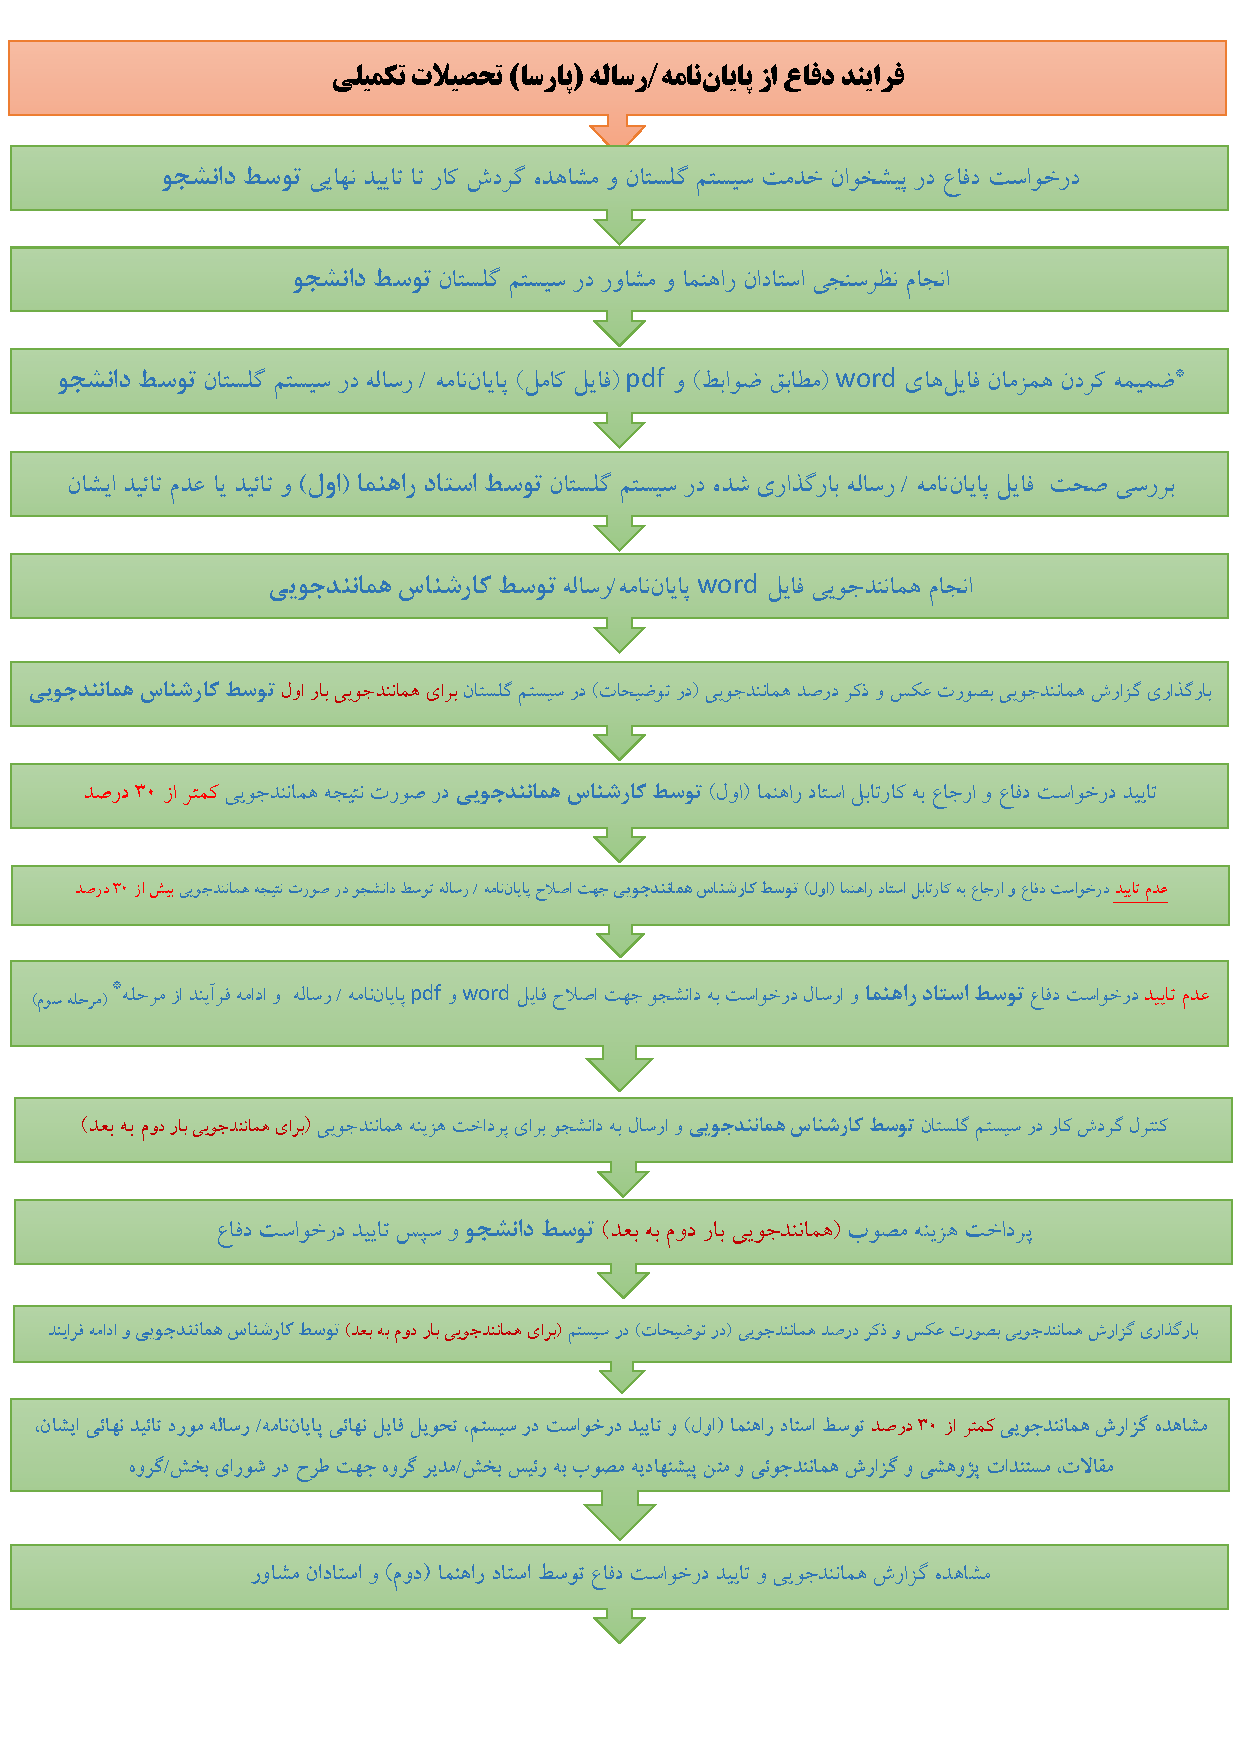
\includegraphics[width=0.95\textwidth]{defence-chart_Part1}}

\centerline{\includegraphics[width=\textwidth]{defence-chart_Part2}}

\section{توصیه‌های تحصیلات تکمیلی دانشگاه در خصوص پارساها}
این دستورالعمل به منظورآشنایی و آگاهی دانشجویان با نحوه نگارش و چگونگی تدوین و تنظیم مطالب یک تحقیق علمی (رساله) 
تهیه شده و ضروری است دانشجویان نکات مطرح شده در آن را هنگام تنظیم رساله رعایت نمایند.

\subsection{ بخش‌های رساله }

رساله باید مشتمل بر بخش‌های زیر باشد: 
\begin{enumerate}
\item شناسنامه یا صفحه عنوان (به زبان فارسی)
\item  شروع با ذکر نام خداوند
\item  صورت‌جلسه (فارسی) هیأت داوران جلسة دفاع از رساله 
\item  تعهدنامۀ رعایت حقوق معنوی دانشگاه یزد
\item  منشور اخلاق پژوهش
\item  تقدیم (اختیاری)
\item  سپاس و قدردانی (اختیاری)
\item  چکیده فارسی  
\item  فهرست مطالب
\item  فهرست شکل‌ها (در صورت داشتن شکل یا نمودار)
\item  فهرست جدول‌ها (در صورت داشتن جدول)
\item  فهرست نمادهای اختصاری و اختصارات (در صورت داشتن علائم، اختصارات و نمادهای اختصاری)
\item  پیشگفتار (اختیاری و با تصویب پردیس/دانشکده مستقل)
\item  متن اصلی که مشتمل بر فصل‌های مختلف از جمله مقدمه یا دیباچه، مروری بر منابع و مطالعات انجام شده و اهداف پژوهش، روش تحقیق، نتایج و تجزیه و تحلیل و تفسیر آنها، نتیجه‌گیری و پیشنهادها است. (مقدمه، فصل اول تلقی می‌شود.)
\item  واژه‌نامه فارسی به انگلیسی یا بالعکس (اختیاری و با تصویب پردیس/دانشکده مستقل و تایید شورای تحصیلات تکمیلی دانشگاه)
\item  فهرست منابع و مآخذ
\item  پیوست‌ها (در صورت وجود)
\item ABSTRACT (چکیده به زبان انگلیسی)
\item  شناسنامه یا صفحه عنوان (به زبان انگلیسی)
\end{enumerate}

\subsection{ حروف‌نگاری (تایپ) رساله}
\begin{enumerate}
 \item برای تایپ رساله از نرم‌افزار Word (نسخه 2013 یا بالاتر) یا LATEX استفاده شود و ترجیحاً متن اصلی با قلم 
BNazanin 14 (یا فونت مصوب پردیس/ دانشکده مستقل با تأیید شورای تحصیلات تکمیلی دانشگاه) باشد. 
متون انگلیسی با قلم \lr{Times New Roman 12} تایپ شود. برای تایپ رساله‌های رشتۀ ادبیات عرب ترجیحاً از قلم 
بدر عربی 15 استفاده شود.

\begin{center}
\begin{tabular}{|c|c|c|} \hline
نوع متن &	فونت فارسی	& فونت انگلیسی \\ \hline
متن عادی &	\lr{BNazanin 14}&	\lr{Times New Roman 12}\\ \hline
شماره صفحه‌ها	& \lr{BNazanin 12}	& \lr{Times New Roman 10}\\ \hline
عنوان فصل‌ها&	\lr{BNazanin Bold 18}	& \lr{Times New Roman Bold 16}\\ \hline
عنوان بخش‌ها	& \lr{BNazanin Bold 16}	& \lr{Times New Roman Bold 14}\\ \hline
عنوان زیربخش‌ها	& \lr{BNazanin Bold 14}	&\lr{Times New Roman Bold 12}\\ \hline
عنوان شکل‌ها/نمودارها و جدول‌ها	& \lr{BNazanin 12}	&\lr{Times New Roman 11}\\ \hline
سربرگ (Header) هر فصل &	\lr{BNazanin 12}	& \lr{Times New Roman 11}\\ \hline
\end{tabular}
\end{center}

\item  در صفحه‌های سمت چپ فایل رساله، فاصله شروع خط تا لبه راست صفحه 4 سانتیمتر -به غیر از سطر مطلع پاراگراف 
که تا لبه صفحه پنج سانتیمتر باشد. فاصله خط تا لبه بالای صفحه سه سانتیمتر، لبه پایین و لبه چپ صفحه 5/2 سانتیمتر باشد. 
در صفحه‌های سمت راست، فاصله شروع خط تا لبه راست صفحه 5/2 سانتیمتر ـ به‌غیر از سطر مطلع پاراگراف که تا لبه صفحه
 5/3 سانتیمتر باشد ـ فاصله خط تا لبه بالای صفحه سه سانتیمتر، لبه پایین صفحه 5/2 و لبه چپ 4 سانتیمتر باشد. 
 فاصله عنوان مطلب تا اولین سطر نوشـته شده 2 سانتیمتر و فاصله بین خطوط 1 سانتیمتر 
 (\lr{Line Spacing: Exactly 29 pt}) باشد. فاصله شماره صفحه از لبه پایین صفحه 1 سانتیمتر باشد. 
 این فواصل برای خطوط در تمام مراحل تدوین رساله اعم از شکل‌ها / نمودارها، جداول، فهرست، عکس‌ها و غیره باید رعایت شود.
\item  
 جدول‌هایی که در راستای طولی صفحه تنظیم می‌شوند، باید طوری قرار گیرند که متن بالای آنها در سمت عطف رساله واقع شود
 و همچنین شکل‌هایی که در راستای طولی صفحه تنظیم می‌شوند، باید طوری قرار گیرند که متن پایین آنها در سمت لبه 
 رساله قرار گیرد. شکل‌ها و جدول‌ها حتی‌المقدور داخل متن و در نزدیک‌ترین فاصله به محلی که ذکر شده، آورده شوند.

توجه: در تدوین و تایپ صفحه‌های رساله به غیر از صفحه‌های تقدیم و سپاسگزاری از هیچ‌گونه کادر تزئینی و تذهیب استفاده نگردد.
\item 
 سعی شود تا حد امکان از به کار بردن واژه‌های با الفبای انگلیسی در متن رساله فارسی خودداری شود و در صورت نیاز، 
معادل انگلیسی لغت‌ها، اصطلاح‌های فارسی یا افراد خاص به صورت پانویس در صفحه‌ مربوطه درج شود (فقط یک‌بار و 
در اولین بار استفاده از آن کلمه). 
پانویس‌ها زیر یک خط که به فاصله‌ 5/2 سانتیمتر از لبه چپ صفحه و حداقل 3 سانتیمتر از لبه پایینی و به طول مورد نیاز 
رسم می‌شود، نوشته شوند. (در هر صورت لازم است 5/2 سانتیمتر حاشیه پایین صفحه رعایت شود). پانویس‌ها در هر صفحه 
با گذاردن شماره 1، 2 و ... در گوشه‌ بالای انتهای کلمه در متن مشخص شوند. (در مورد اصطلاحات و عبارت‌های علمی، توصیه 
شود که تا حد امکان از معادل فارسی مناسب استفاده شود و در مورد اسامی افراد خارجی هم از روال یکسانی برای همه اسامی 
استفاده شود).
\item 
 در نگارش کلماتی نظیر آن‌ها و ... که از دو بخش تشکیل شده است ولی یک کلمه (یا مفهوم) محسوب می‌شود بایستی ارتباط 
بین دو بخش به‌صورت "جداکننده بدون فاصله" (فشردن کلیدهای Shift+Space بصورت همزمان در صفحه کلید استاندارد 
فارسی) رعایت شود.
\item 
 برای قرار دادن علائم نگارشی نظیر نقطه، ویرگول، علامت سوال، علامت تعجب و ... بایستی بین این علائم و کلمات قبل 
فاصله‌ای نباشد ولی بعد از آن یک فاصله ایجاد شود.
\item 
 در مورد پرانتز، بین عبارت‌های داخل پرانتز و پرانتز فاصله‌ای نباشد، اما بین پرانتزها و عبارت‌های دو طرف آن یک فاصله 
قرار گیرد.
\item 
 نوشتن کلماتی مانند به‌جز، به‌سرعت، به‌دقت و ... به‌صورت بجز، بسرعت، بدقت و ... اشتباه است و بایستی بصورت مجزا 
و با رعایت نیم‌فاصله نوشته شوند. برای اطلاع از جزئیات بیشتر می‌توان به منابعی نظیر "دستورخط فارسی"، "به‌نویسی" 
و... مراجعه کرد.
\item 
 علامت نقطه-ویرگول (؛) یا مکث میانه در مواردی استفاده می‌شود که مفهوم جمله ناتمام است.
\item 
 سعی شود از نوشتن پاراگراف‌های طولانی اجتناب شود. 
\item 
 توصیه می‌شود در انتهای هر فصل به‌جز فصل مقدمه، یک بخش جمع‌بندی یا خلاصه فصل وجود داشته باشد. (با تایید پردیس/ دانشکده مستقل).
\item 
 توصیه می‌گردد برای نوشتن فرمول‌ها و روابط ریاضی در نرم‌افزار Word، از افزونه یا نرم‌افزار Mathtype استفاده شود.
\item 
 فهرســت مطالب ارائه شده با توجه به قالب مورد تایید هر دانشکده/ گروه مستقل می‌تواند متفاوت از نمونه ذکر شده در این فایل باشد.
\item 
 توصیه می‌شود عنوان هر فصل بالای صفحات مربوط به آن فصل به‌صورت سربرگ (Header) آورده شود. 
\end{enumerate}
\subsection{ شماره‌گذاری}
\begin{enumerate}
\item  شماره‌گذاری صفحه‌ها

در هنگام شماره‌گذاری صفحه‌های رساله، موارد قبل از فهرست مطالب (موارد 1 الی 8 قسمت الف) هیچگونه شماره‌ای داده نشود. 
شماره‌گذاری فهرست‌ها و پیشگفتار با استفاده از حروف ابجد یا اعداد رومی انجام شود و شماره‌گذاری متن اصلی با استفاده از اعداد 
فارسی تا آخرین صفحه انجام شود. توجه گردد در صفحۀ اول هر فصل که عنوان فصل نوشته می‌شود، شماره‌ صفحه ذکر نشود، 
لیکن به حساب آید. شماره‌گذاری صفحه‌ها باید وسط و به فاصله 1 سانتیمتر از لبه پایین صفحه باشد.
\item 
 شماره‌ گذاری فصل‌ها، بخش‌ها و زیربخش‌ها

بخش‌ها و زیربخش‌های مختلف هر فصل با اعدادی نظیر 6-4 یا 6-4-2 مشخص می‌شود که عدد 6 شماره‌ فصل، عدد 4 شماره 
بخش و عدد 2 شماره قسمت است. شماره و عنوان هر فصل با قلم \lr{BNazanin 18 Bold} و عناوین بخش‌های مختلف 
هر فصل با قلم \lr{BNazanin 16 Bold} و عناوین قسمت‌های هر بخش با قلم \lr{BNazanin 14 Bold}
 تایپ شود (یا فونت‌های مصوب پردیس/ دانشکده مستقل و تأیید شورای تحصیلات تکمیلی دانشگاه). ضمناً عناوین فصل‌ها 
 و بخش‌های زیر فصل حتماً به صورت خودکار با استفاده از levelهای word تنظیم گردند.
\item 
 شماره‌ گذاری جدول‌ها، شکل‌ها 

برای شماره‌گذاری جدول‌ها و شکل‌ها در متن اصلی رساله از دو شماره که با خط فاصله از یکدیگر جدا می‌گردند، استفاده 
می‌شود به‌طوری‌که تمام جدول‌ها و شکل‌ها از ابتدا تا انتهای رساله به ترتیب دارای شماره 1، 2، ... و n برای هر فصل خواهند 
بود که شماره سمت چپ نشان‌دهنده ترتیب جدول / شکل و شماره سمت راست نشان‌دهنده شماره فصلی است که جدول / شکل 
در آن ذکر گردیده است. (مثلاً برای فصل 2: جدول 2-1، جدول 2-2 و ...، برای فصل 3: جدول 3-1، جدول 3-2 و ...). شماره‌گذاری 
جدول-ها، شکل‌ها و.... مستقل از همدیگر صورت می‌گیرد (البته قابل ذکر است که «نمودار»ها هم جزء «شکل»ها تلقی می شوند و نیاز
 به تیتر (عنوان) مجزایی ندارند). عنوان جدول‌ها در بالای آنها و عنوان شکل‌ها در زیر آنها ذکر می‌گردد.
شماره‌ای که در متن به شکل‌ها، جدول‌ها و ... اختصاص داده می‌شود، باید به همان صورت، در فهرست جدول‌ها، شکل‌ها و ... 
که قبل از شروع متن اصلی در رساله تنظیم می‌گردد، ذکر شود. فهرست مطالب، فهرست شکل‌ها و فهرست جدول‌ها و... به 
صورت خودکار در word ایجاد شود.
\item 
 شماره ‌گذاری روابط و فرمول‌ها

 فرمول‌ها در هر فصل به طور جداگانه و به ترتیبی که ظاهر می‌شوند (مانند جدول‌ها و شکل‌ها)، شماره‌گذاری گردد. 
 شماره‌گذاری روابط و فرمول‌های نوشته شده در متن اصلی رساله مشابه با جدول‌ها و شکل‌ها از ابتدا تا انتهای رساله به 
 ترتیب 1، 2، ... و n برای هر فصل و در پرانتز لحاظ خواهند شد. به‌طور مثال فرمول بیستم در فصل سوم به‌صورت (3-20) 
 نوشته می‌شود.
در مورد شماره‌گذاری قضیه‌ها، گزاره‌ها، لم‌ها، مثال‌ها و نظایر آنها در هر فصل به‌طور جداگانه و به-ترتیبی که در متن می‌آیند 
شماره‌گذاری می‌شوند؛ این شماره‌گذاری چنان است که شماره فصل در سمت راست و شماره قضیه (و نظایر آن) بعد از آن آورده
 شده و بین آنها از نقطه استفاده می‌شود. لازم است کلمه قضیه (و نظایر آن) و شماره آنها به صورت قلم سیاه (Bold) نوشته شده
 و پس از آن علامت دو نقطه (:) آورده شود. همچنین برای شروع اثبات کلمه اثبات همراه (:) به صورت قلم سیاه می‌آید؛ (معمولا 
 برای رشته‌های دانشکده علوم ریاضی و ...)
\end{enumerate}
\subsection{منابع و مآخذ}

لازم است در متن به کلیه منابعی که مورد استفاده قرار می‌گیرد، اشاره شود. مرجع دهی باید بر اساس قالب مورد تصویب 
دانشکده / گروه مستقل باشد و اگر دانشکده / گروه مستقل قالب خاصی را تعیین نکرده، از قالب APA استفاده شود.
در صورتی‌که از نرم‌افزار مدیریت مرجع استفاده نمی‌شود معمولا به یکی از دو روش زیر در متن به مراجع اشاره می‌گردد:

\begin{enumerate}
\item  مراجع به ترتیبی که در متن می‌آیند شماره‌گذاری شوند. در این روش، مراجع به ترتیب شماره در فهرست 
منابع و مآخذ ذکر گردد. 
\item 
مراجع به ترتیب حروف الفبایی نام خانوادگی نویسنده اول شماره‌گذاری گردیده، به همین ترتیب در فهرست منابع و مآخذ 
ذکر می‌شود.
القاب و عناوین دکتر، مهندس و … از جلوی نام مؤلف، مترجم حذف می‌گردد و همچنین اگر کتاب دارای دو نویسنده یا 
بیشتر باشد نام و نام خانوادگی همه آنها به ترتیبی که در روی جلد کتاب آمده است، آورده شود.

به‌طور مثال:

یاحقی، محمد جعفر و ناصح، محمد مهدی، راهنمای نگارش و ویرایش، چاپ هشتم، مشهد: آستان قدس رضوی، ص106.

در صورت وجود منابع به زبان‌های مختلف، توصیه‌ می‌شود مراجع غیرانگلیسی نیز به انگلیسی ترجمه و در 
انتها واژه‌ی (\lr{in Persian}) داخل پرانتز قید شده و سال آنها نیز به میلادی برگردان شوند. در غیر این صورت، 
ابتدا مراجع فارسی و سپس سایر مراجع ذکر شود. 
اگر شکل یا جدولی از منبع و مأخذی گرفته شده، لازم است مرجع آن در انتهای عنوان آن شکل یا جدول آورده شود.
\end{enumerate}
\subsection{شیوه‌نامه پردیس فنی و مهندسی}
برای دانشجویان پردیس فنی و مهندسی رعایت موارد ذیل الزامی است.
\begin{enumerate}
\item  استفاده از نرم‌افزار مدیریت مرجع مانندEndnote ، Mendeley و ... الزامی است.
\item  برای ارجاع بصورت شماره از قالب IEEE  و برای ارجاع با استفاد از نام و تاریخ از قالب APA استفاده شود.
\item  در صورت وجود منابع به زبان‌های مختلف، ضروری است مراجع غیرانگلیسی نیز به انگلیسی ترجمه و در انتها واژه‌ی
 (in Persian) داخل پرانتز قید شده و سال آنها نیز به میلادی برگردان شوند.
\end{enumerate}
\section{آماده‌سازی فایل جهت همانندجویی}
با توجه به نیاز به همانندجویی پیشنهادیه و پارساهای دانشگاه، لازم است کلیه دانشجویان در زمان درخواست دفاع با تصویب پیشنهادیه، 
فایل پیشنهادیه/پایان‌نامه با فرمت Word را در سامانه گلستان بارگذاری نمایند تا همانندجویی روی آن‌ها  انجام شود. 

برای دانشجویانی که از زیپرشن برای تایپ پایان‌نامه استفاده کرده‌اند، کافی است محتویات فایل \lr{.tex} را که محتوای پایان‌نامه آنها است را به 
همان صورت کپی و در یک فایل Word الصاق نمایند و فایل Word حاصل را برای همانندجویی بارگذاری دهند. لازم به ذکر است که نیاز به 
صفحات اولیه و مراجع پیشنهادیه/پایان‌نامه برای همانندجویی نیست.
 
راهکار دیگری که پیشنهاد می‌شود و البته مستلزم استفاده از ابزاری به نام GrindEQ است، این است که با نصب این ابزار، فایل اصلی پیشنهادیه/پایان‌نامه 
را در Word باز نمایید تا تمام پایان‌نامه به Word تبدل شود. البته این ابزار مجانی نیست، ولی برای هر نصب، تا 10 تبدیل را انجام می‌دهد. 
با این تبدیل، تمام فرمول‌ها و غیره کاملا منتقل می‌شود. تنها مشکل آن، نداشتن ساختار است و شکل‌ها نیز بعضا منتقل نمی‌شود که می‌شود دستی اصلاح 
کرد. البته برای همانندجویی، نیازی به داشتن شکلها نیست. راهنمای نصب و استفاده از این ابزار در بخش~\label{sec:grineq} آمده است.

%\newpage 
\subsection{ دستورالعمل ورود اطلاعات پایان‌نامه کارشناسی ارشد/ رساله دکتری توسط دانشجو در سامانه \lr{Irandoc}}
% پژوهشگاه علوم و اطلاعات ایران (Irandoc)}

\centerline{\includegraphics[width=0.6\textwidth]{Irandoc}}
\pagebreak 

\subsection{برخی نکات نگارشی}
در نوشتن مطالب علمی، رعایت قوانین نگارشی لازم است. در این کوتاه، صرفاً به برخی نکات نگارشی مهم اشاره می‌شود که لازم است در متن
پارساها به آن‌ها توجه شود. لازم به ذکر است که در خصوص برخی از قوانین نگارشی، ممکن است اختلاف نظری وجود داشته باشد ولی اکثر موارد 
ذکرشده مورد اتفاق است.
\begin{enumerate}
\item  علائم سجاوندی مانند کاما، ؛، .، :، ! و ؟ بدون فاصله با کلمه‌ی قبل از خود نوشته می‌شوند، ولی بعد از
آن‌ها باید یک فاصله‌ی خالی قرار گیرد. مانند: من، تو؛ او.
\item 
 علامت‌های پرانتز، آکولاد، کروشه، نقل‌قول و نظایر آن‌ها، بدون فاصله با عبارت داخل خود نوشته 
می‌شوند، ولی با عبارت اطراف خود یک فاصله دارند. مانند: (اين)،  (آن) و «آن‌ها».
\item 
  علامت استمرار «می» جدای از کلمه‌ی بعد خود و بی‌فاصله با آن (یعنی با نیم‌فاصله) نوشته می‌شود. مانند: می‌دهیم، می‌شود.
\item 
 علامت جمع «ها»، علامت صفت برتری «تر» و علامت صفت برترین «ترین»؛ جدای از کلمه‌ی قبل از خود و بی‌فاصله با آن  (یعنی با نیم‌فاصله) نوشته می‌شود. 
 مانند: آن‌ها بیش‌تر و کم‌ترین.
 
تبصره: کلمه‌های بهتر و بهترین از این قاعده مستثنا هستند.
\item 
 شناسه‌های «ام». «ایم»» «ای». «اید» و «اند» بی‌فاصله با کلمه‌ی قبل از خود  (یعنی با نیم‌فاصله) نوشته می‌شوند. ولی «است» با
فاصله است، مگر وقتی که کلمه‌ی قبلی با «ه» یا «ا» تمام شود. مانند: رفته‌ام رفته است. از ماست که برماست.
\item 
 ضمیرهای متصل جمع جدا ولی بدون فاصله با کلمه‌ی قبل خود  (یعنی با نیم‌فاصله) نوشته می‌شوند. مانند: زندگی‌مان؛
راه‌شان» ولی ضمیرهای متصل مفرد متصل نوشته می‌شوند. مانند: راهم نامت و کتابش.
\item 
 «به» هميشه جدا از کلمه‌ی قبل از خود ولی بدون فاصله  (یعنی با نیم‌فاصله) نوشته می‌شود. مگر در مواری که فعل ساخته
شود. مانند: به‌نام، به‌سزا، ببینیم.
\item 
 «به» هم‌واره جدا از کلمه‌ی قبل از خود ولی بدون فاصله نوشته می‌شود. مگر در مواری که حرف
اضافه‌ی «به» به تنهایی به‌کار رفته باشد. مانند: به‌سوی, به‌طرف، به آن‌ها.
\item 
‏ اجزای فعل با فاصله نوشته می‌شوند، مگر وقتی که یک جزء آن حرف اضافه باشد که در آن ‌صورت؛
حرف اضافه با کلمه‌ی بعد فاصله نخواهد داشت. مانند: تحریر کردن، درآورده شد، برآمده است، به‌کار
‏گرفتن.
\item 
 پیشوندها و پسوندهای جامد سرهم نوشته می‌شوند. مانند: دانشگاه، همسایه، همسر.
 
تبصره: در مورادی که خواندن کلمه دچار اشکال شود، می‌توان پسوند و پیشوند را جدا کرد. مانند: هم‌میهن، هم‌ارزی.
\item 
 اجزای حروف اضافه‌ی مرکب، قیدها، اسم‌ها، و صفت‌های مرکب بی‌فاصله نوشته می‌شوند. مانند: دراین‌صورت، آن‌گاه، به‌طوری‌که، کتاب‌خانه، دانش‌جو.
 \item 
 کلمه‌های مرکب دیگر نیز جدا و بدون فاصله نوشته می‌شوند. مانند: گفت‌وگو، پرس‌وجو و جست‌وجو.
 \item 
به‌دلیل دشواری خواندن، می‌توان «ها»ی ملفوظ را از قوانین جداسازی استثنا نمود. مانند: راهنما؛ رهبر.
\item 
 کسره‌ی اضافه‌ی بعد از «ه» به‌صورت «ه‌ی» نوشته می‌شود، نه «ۀ». مانند: خانه‌ی علی.
 
تبصره: اگر «ه» ملفوظ باشد. نباید «ی» را نوشت. مانند: فرمانده کل، پادشه خوبان.
\item 
 پایه‌های همزه در کلمه‌ها همیشه «ئ» است. مگر در مواری که همزه ساکن باشد. که دراین‌صورت باید
متناسب با اعراب حرف قبل نوشته شود. مانند: مسئله، مسئول، رأس، مؤمن.

تذکر: همزه‌ی بعد از حرف کشیده‌ی «ا» نوشته نمی‌شود. مانند: املا، استقرا، استثنا.
\item 
سعی شود جمع‌های کلمه‌های عربی به فارسی نوشته شود. مانند: شکل‌ها (به‌جای اشکال)، عبارت‌ها (به‌جای عبارات)، علامت‌ها (به‌جای علائم).
\item 
 جملات نقل‌قول یا موکد درون علامت نقل‌قول « و » قرار می‌گیرند. نه بین " *. مانند «استعداد خوب».
\item 
کلمه‌هایی که با جدانویسی خواناترند. جدا و بدون فاصله نوشته می‌شوند. مانند: چه‌گونه (به‌جای چگونه).
\item 
 «ی» عربی به‌صورت «» نوشته می‌شود. مگر آن‌که خوانند دچار مشکل شود. مانند: حتا و مستثنا.
 \item در کلمه‌های دو بخشی که به همراه هم یک مفهوم را مشخص می‌کنند، از نیم فاصله استفاده شود. مانند خوشه‌بندی، بهینه‌سازی، پیاده‌سازی و پایان‌نامه.
 یک راه  تشخیص، نگاه به کلمه انگلیسی معادل است. مثلاً \lr{clustering}  و \lr{optimization} و \linebreak 
 \lr{implementation} و \lr{thesis}.
 \item در استفاده از کاما برای روان‌تر شدن خواندن جملات استفاده شود. معمولاً هر جا در خواندن جمله یک توقف کوتاه رخ می‌دهد، باید کاما اضافه‌ شود.
 مانند «همچنان که در بخش قبل بیان شد، الگوریتم‌های ابتکاری کاربرد بسیاری در ....»
 \item حتی‌الامکان از معادل فارسی کلمات انگلیسی استفاده شود. مانند روش به جای تکنیک.
\end{enumerate}

\section{چند راهکار ساده اما راهگشا!}
یکی از وقت‌گیرترین کارهای آماده‌سازی یک متن علمی، مخصوصاً  در تجربه‌های اول، وفور خطاهای عمدتاً نگارشی است
که رفع آن‌ها، اولاً وقت زیادی می‌گیرد و ثانیاً نیاز به تمرکز بسیار دارد و حقیقتاً حوصله دانشجویان را به سر می‌برد. در این فصل راهکارهای ساده‌ای
ارائه می‌شود که می‌توانید این روند را سریع و بدون دردسر و با دقت زیاد انجام دهید.

\subsubsection{راهکار اول: از replace استقاده کنید!}
فرض کنید در پایان‌نامه، کلمه «می شود» را به همین صورت اشتباه استفاده کرده‌اید. لذا باید همه موارد استفاده شده به صورت «می شود» را به «می‌شود»
اصلاح نمایید. انجام این کار به صورت دستی و مورد به مورد بسیار مشکل است و در نهایت نیز مواردی از چشم شما پنهان می‌ماند. اما با استفاده از امکان
replace که تقریباً در تمام ادیتورها در دسترس هستند، می‌توانید این کار را در سرتاسر پایان‌نامه با صرف چند دقیقه و بدون نیاز به بررسی چشمی
انجام دهید. برای این کار replace ادیتور خود را انتخاب کنید (این کار در \lr{Notepad++} با کلید میانبر \lr{CTRL+H} می‌توانید انجام دهید).
سپس در قسمت \lr{Find}،  کلمه «می شود» و در قسمت \lr{Replace with}، کلمه «می‌شود» (هر دو بدون گیومه اول و آخر) قرار دهید. سپس گزینۀ
\lr{Find} را کلیک کنید و کلمه «می شود» بعدی را ببینید و اگر مایل به جایگزین هستید، گزینه \lr{Replace} را انخاب کنید. تکرار انتخاب ترتیبی
گزینه‌های \lr{Find} و \lr{Replace} به ترتیب اشکالات را پیدا و رفع می‌نماید. این کار را در تمام فایل‌های مربوط به پایان‌نامه خود تکرار کنید. اگر
از عدم وجود ترکیب‌های مشابه اطمینان دارید، می‌توانید با انتخاب گزینۀ \lr{Replace All}، همه اصلاحات را بدون چک کردن انجام دهید ولی برای 
استفاده از این گزینه دقت کنید زیرا ممکن است ترکیب مورد نظر شما در کلمات دیگری هم باشد که مایل به تغییر آن‌ها نباشید.

\subsubsection{راهکار دوم: استفاده از \lr{Inverse-Search}}
یکی از مشکلات کار با لاتک در مقایسه با \lr{Word} این است که متن نهایی با  متن نوشته شده متفاوت است. لذا اگر جایی از متن نیاز به
اصلاح داشته باشد، باید محل متناظر را در فایل tex یافت و سپس آن را اصلاح کرد. این کار، مخصوصاً اگر سند ما مفصل و چند ده صفحه‌ای باشد، بسیار
وقت‌گیر و خسته کننده است. اما اگر از \lr{SumatraPDF} استفاده کنید و نام پوشه و ابرپوشه‌های حاوی فایل سند شما فارسی نباشد، به راحتی با 
دوبار کلیک روی هر محل در فایل پی دی اف که در نرم‌افزار \lr{SumatraPDF} باز شده است، به محدوده همان محل در فایل tex مربوطه
منتقل می‌شوید. با این کار، عملاً نیاز به جستجوی طولانی مدت برای پیدا کردن محل ندارید.

\subsubsection{راهکار سوم: خطایابی و رفع خطا در بازه‌های زمانی کوتاه}
همانطور که در فیلم‌های آموزشی دوره مقدماتی لاتک آمده است، لاتک اصولاً یک زبان برنامه‌نویسی است که برای حروف‌چینی متون است. لذا، مشابه
یک برنامه، در صورت رعایت نشدن فرمت دستورات آن، در زمان حروف‌چینی با خطا مواجه خواهید شد. این خطا ممکن است به دلایلی نظیر
فراموش شدن یک علامت $\$$ یا  $\}$ باشد. البته، لاتک در صورت بروز خطا، تا بتواند کار را انجام می‌دهد اما اگر خطا به گونه‌ای باشد که کل کار را
مختل نماید، ممکن است بخشی یا کل متن حروف‌چینی نشود و در فایل پی دی اف نهایی نیاید. همانطور که در برنامه‌نویسی توصیه می‌شود، توصیه این است
که در زمان تایپ متن، در دوره‌های کوتاه‌مدت، متن را حروف‌چینی کنید و در صورت بروز خطا، آن را برطرف نمایید و پس از برطرف کردن کامل
خطاها، تایپ بخش بعدی را شروع نمایید. با این کار محدوده شما برای خطایابی کوچک بوده و معمولاً خطاها به سرعت پیدا و اصلاح می‌شوند.
\subsubsection{راهکار چهارم: گرفتن منظم نسخۀ پشتیبان}
هرچند فایل‌های لاتک، متنی هستند و مشابه فایل‌های ابزارهای مثل \lr{Word} نیستند که خراب شوند، ولی حذف شدن فایل یا رونویسی شدن
آن‌ها می‌تواند باعث از دست رفتن بخشی از کار شود. لذا توصیه کلی این است که نسبت به نسخه پشتیبان گرفتن از فایل‌های خود به طور منظم و در فواصل
نه چندان طولانی اقدام نمایید. همچنین می‌توانید ادیتور مورد استفاده خود را بررسی کنید و در صورت داشتن امکانات ایجاد فایل‌های پشتیبان به صورت
خودکار، آن را فعال نمایید.!
داخل فایل
\LRE{\verb!yazd-thesis-template.tex!}
و بعد از دستور
\verb!\chapter{راهنمای استفاده از کلاس \lr{yazd-thesis}}
\section{مقدمه}
حروف‌چینی پایان‌نامه یا رساله یکی از موارد پرکاربرد استفاده از زی‌پرشین است. از طرفی، یک  پایان‌نامه یا رساله،  احتیاج به تنظیمات زیادی از نظر صفحه‌آرایی  دارد که ممکن است برای
یک کاربر مبتدی، مشکل باشد. به همین خاطر، برای راحتی کار کاربر، کلاس حاضر با نام 
 \LRE{\verb!yazd-thesis!}
 برای حروف‌چینی پروژه‌ها، پایان‌نامه‌ها و رساله‌های دانشگاه یزد با استفاده از نرم‌افزار زی‌پرشین،  آماده شده است. این فایل به 
گونه‌ای طراحی شده است که کلیه خواسته‌های مورد نیاز  مدیریت تحصیلات تکمیلی دانشگاه یزد را برآورده می‌کند. همچنین حروف‌چینی بسیاری
از قسمت‌های آن، به طور خودکار انجام می‌شود.

کلیه فایل‌های لازم برای حروف‌چینی با کلاس گفته شده، داخل پوشه‌ای به نام
 \LRE{\verb!yazd-thesis!}
  قرار داده شده است. توجه داشته باشید که برای استفاده از این کلاس باید فونت‌های \lr{Yas}، \lr{Times New Roman}، 
  \lr{B Nazanin}  و \lr{Titr} روی کامپیوتر شما نصب باشد. این فونت‌ها در بین فونت‌های مشخص شده جهت نصب وجود دارد، ولی با توجه به این که
  ممکن است نصب \TeX{}Live از طریق دیگری انجام شده باشد، فونت‌های لازم در مسیر Fonts قرار گرفته است. می‌توانید این فونت‌ها را روی سیستم‌عامل
  خود نصب نمایید. تاکید می‌شود، در صورت نصب فونت، اگر با پیام وجود فونت روی کامپیوتر خود مواجه شدید، گزینه رونویسی فونت را انتخاب کنید تا از
  استفاده از نگارش مناسب فونت‌ها اطمینان حاصل نمایید.
 
\section{این همه فایل؟!}\label{sec2}
از آنجایی که یک پایان‌نامه یا رساله، یک نوشته بلند محسوب می‌شود، لذا اگر همه تنظیمات و مطالب پایان‌نامه را داخل یک فایل قرار بدهیم، باعث شلوغی
و سردرگمی می‌شود. به همین خاطر، قسمت‌های مختلف پایان‌نامه یا رساله  داخل فایل‌های جداگانه قرار گرفته است. مثلاً تنظیمات  کلاس داخل فایل
\LRE{\verb!yazd-thesis.cls!}، 
قسمت مشخصات فارسی پایان‌نامه داخل 
\LRE{\verb!fainfo.tex!}،
مطالب فصل اول، داخل 
\verb!chapter1!
و ... قرار داده شده است. نکته مهمی که در اینجا وجود دارد این است که از بین این  فایل‌ها، فقط فایل 
\LRE{\verb!yazd-thesis-template.tex!}
قابل اجرا است. یعنی بعد از تغییر فایل‌های دیگر، برای دیدن نتیجه تغییرات، باید این فایل را اجرا کرد. بقیه فایل‌ها به این فایل، کمک می‌کنند تا بتوانیم خروجی کار را ببینیم. اگر به فایل 
\LRE{\verb!yazd-thesis-template.tex!}
دقت کنید، متوجه می‌شوید که قسمت‌های مختلف پایان‌نامه، توسط دستورهایی مانند 
\verb!input!
و
\verb!include!
به فایل اصلی، یعنی 
\LRE{\verb!yazd-thesis-template.tex!}
معرفی شده‌اند. بنابراین، فایلی که همیشه با آن سروکار داریم، فایل 
\LRE{\verb!yazd-thesis-template.tex!}
است.
در این فایل، فرض شده است که پایان‌نامه یا رساله، از ۳ فصل و یک پیوست، تشکیل شده است. با این حال، اگر
  پایان‌نامه یا رساله، بیشتر از ۳ فصل و یک پیوست است، باید خودتان فصل‌های بیشتر را به این فایل، اضافه کنید. این کار، بسیار ساده است. فرض کنید بخواهید یک فصل دیگر هم به پایان‌نامه، اضافه کنید. برای این کار، کافی است یک فایل با نام 
\verb!chapter4!
و با پسوند 
\verb!.tex!
بسازید و آن را داخل پوشه 
\LRE{\verb!yazd-thesis!}
قرار دهید و سپس این فایل را با دستور 
\verb!\chapter[برخی نکات مفید]{ برخی نکات مفید ( اضافه کردن عنوان برای بیش از یک خط شدن)}
\twocolumnfootnotes
\section{فرایند تصویب پیشنهادیۀ پارسای تحصیلات تکمیلی}
در این بخش، فرآیند تصویب پیشنهادیۀ پایان‌نامه/رساله آورده شده است. 
دستورالعمل کامل مراحل تصویب و ثبت پیشنهادیۀ پایان‌نامه/ رساله دانشجویان تحصیلات تکمیلی در پیوست~\ref{ch:proposal}
آمده است.

لطفا برای مشاهده آخرین تغییرات به وبسایت تحصیلات تکمیلی دانشگاه به آدرس

\centerline{\url{https://yazd.ac.ir/offices/educational/deputy/graduate/home/rules}}

مراجعه نمایید.

\centerline{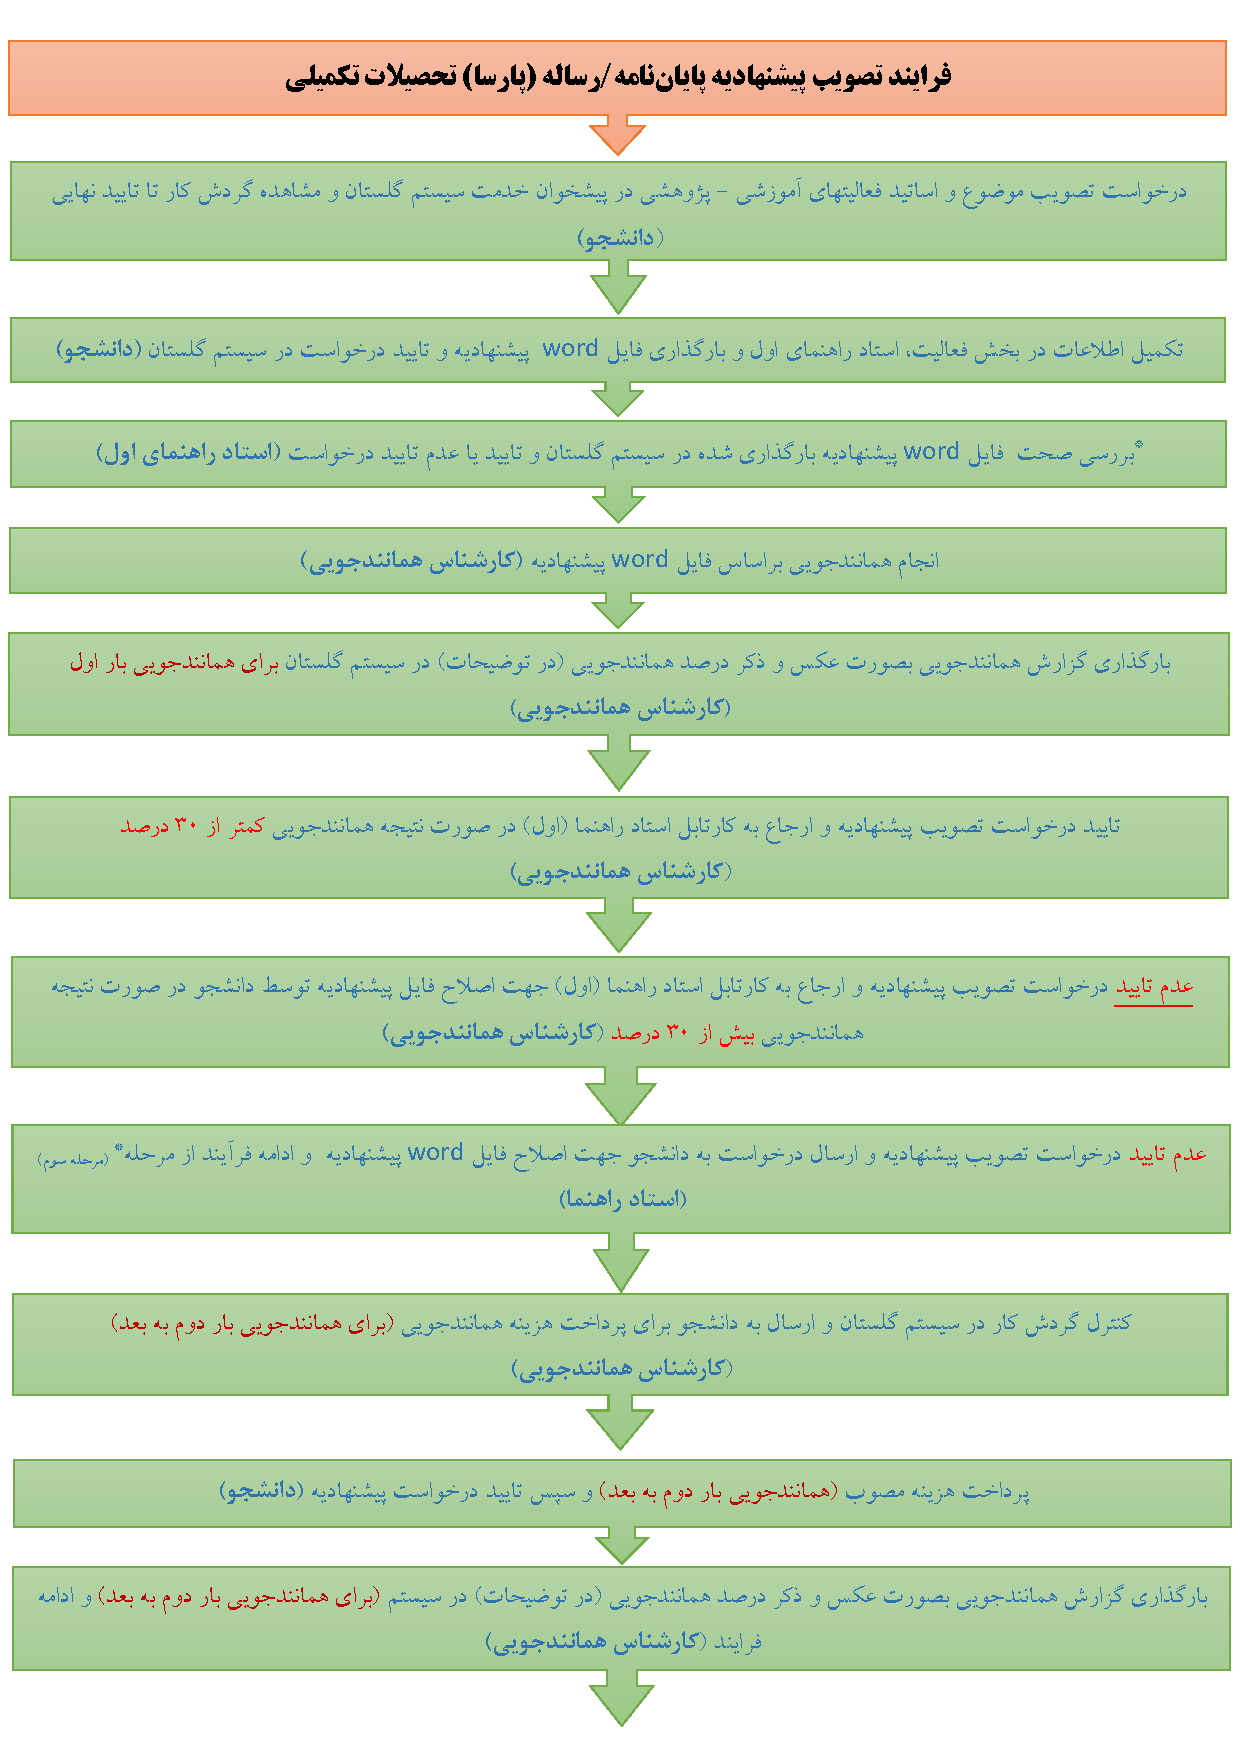
\includegraphics[width=0.9\textwidth]{Proposal-chart_Part1}}

\centerline{\includegraphics[width=\textwidth]{Proposal-chart_Part2}}

\section{دستورالعمل نحوه برگزاری جلسات دفاع }
\subsection{هدف }
هدف از تدوین این دستورالعمل ایجاد نظم و ترتیب بیشتر و شفاف‌سازی چگونگی برگزاری جلسات دفاع پایان‌نامه 
کارشناسی ارشد و رساله دکتری  و یادآوری نکات مهم برای برگزاری جلسه مطابق مقررات و شیوه‌نامه‌های تحصیلات تکمیلی‌است 
که بر اساس صورتجلسه شورای تحصیلات تکمیلی دانشگاه مورخ 17/2/1397 توسط نماینده تحصیلات تکمیلی (ناظر جلسه دفاعیه) 
دانشگاه مدیریت می‌گردد. 

\subsection{الف) فرآیند دفاع از پایان‌نامه / رساله }

\begin{enumerate}
\item  دانشجو: درخواست دفاع در پیشخوان خدمت

دانشجو در این قسمت ضمن درخواست دفاع‏، تاریخ و محل پیشنهادی دفاع از پایان‌نامه / رساله را بر اساس هماهنگی به عمل آمده
 با استادان راهنما / مشاور و پس از تایید اولیه رئیس بخش/ مدیرگروه ثبت می‌نماید. 
برای این منظور لازم است: 

*‌ دانشجو ظرف 48 ساعت، پایان‌نامه / رساله خود را همراه با مقالات مستخرج و تأییدیه‌های مجلات برای طرح در شورا به
 رئیس بخش / مدیرگروه تحویل و پس از تصویب جزئیات دفاع در شورا، فایل پایان‌نامه / رساله تصحیح شده نهایی و دستاوردهای
 مستخرج از آن را برای كارشناس تحصیلات تكمیلی ارسال کرده و فرآیند دفاع را تا مرحله تأیید معاون دانشكده / مدیرگروه مستقل پیگیری می‌نماید. 
 
*‌ برای دانشجویان دکتری لازم است كاربرگ بررسی مقالات از قبل با رعایت ضوابط مربوط تأیید و جلسه پیش دفاع دانشجو
 (حداقل 21 روز قبل از تاریخ دفاع) مطابق مقررات به طور موفقیت‌آمیز برگزار شده باشد و کاربرگ‌های مربوطه تکمیل، تایید و 
 به کارشناس جهت ثبت و بارگذاری در سیستم گلستان تحویل شده باشد.

\item  دانشجو: انجام نظرسنجی 

در این مرحله دانشجو باید نظرسنجی از استادان راهنما و مشاور پایان‌نامه / رساله را انجام و تایید نماید. 

\item  دانشجو: ضمیمه کردن همزمان فایل‌های word و  pdfپایان‌نامه / رساله

در این مرحله دانشجو فایل تصحیح شده نهایی پایان‌نامه / رساله را پیوست و برای انجام فرآیند همانندجویی ارسال می‌نماید. 
لازم به ذکر است فایل pdf  ضمیمه شده همان فایلی است که در اختیار اعضای هیأت داوران قرار می‌گیرد. 

* ضروری است تنها در نسخه word پایان نامه مفاد دستورالعمل بارگذاری رساله/پایان نامه برای همانندجویی رعایت شده باشد.

* هزینه همانندجویی برای مرحله اول به عهده دانشگاه و در سایر مراحل به عهده دانشجو است. 

\item  استاد راهنما: بررسی صحت  فایل پایان‌نامه / رساله بارگذاری شده 

در این مرحله استاد راهنما (اول) فایل پایان‌نامه / رساله بارگذاری شده توسط دانشجو را مشاهده، کنترل و در صورت عدم مغایرت، 
درخواست دفاع را تایید می‌نماید، در غیر اینصورت بایستی با انتخاب گزینه «عدم تایید» درخواست دفاع به کارتابل دانشجو عودت شود
 و دانشجو نسبت به انجام اصلاحات و بارگذاری فایل صحیح پایان‌نامه / رساله مجدداً اقدام نماید. 

\item  کارشناس همانندجویی دانشکده / گروه مستقل: انجام همانندجویی 

5-1- همانندجویی برای بار اول

کارشناس همانندجویی دانشکده / گروه مستقل، متن فایل word پیوست شده توسط دانشجو را در سامانه همانندجویی کپی 
و ارسال و نتیجه را در فایل دانشجو بارگذاری و درخواست را (با ذکر درصد همانندی در توضیحات) تایید / عدم تایید می‌نماید. 
*در صورتی که نتیجه همانندجویی کمتر از 30 درصد باشد، درخواست دفاع دانشجو تایید و به کارتابل استاد راهنما جهت طی 
مراحل بعدی ارجاع می‌شود. 

*در صورتی که نتیجه همانندجویی بیشتر از 30 درصد باشد، درخواست دفاع دانشجو عدم تایید و جهت اصلاح پایان‌نامه / رساله توسط دانشجو، 
به کارتابل استاد راهنما برمی‌گردد. 

5-2- همانندجویی برای بار دوم به بعد

*در صورتی که همانندجویی برای بار دوم به بعد انجام می‌شود (با کنترل گردش کار در گلستان)، کارشناس درخواست دفاع را برای 
پرداخت هزینه همانندجویی به دانشجو ارسال می‌‌نماید. 

5-2-1- دانشجو: پرداخت هزینه همانندجویی بار دوم به بعد

در صورتی که همانندجویی برای بار دوم به بعد انجام می‌شود دانشجو ملزم به پرداخت هزینه مصوب و تایید درخواست دفاع است. 

5-2-2- کارشناس همانندجویی دانشکده / گروه مستقل

 بعد از پرداخت هزینه توسط دانشجو فرآیند همانندجویی مطابق  بخش 5-1- انجام و ادامه می‌یابد. 

\item  استاد راهنما

در این مرحله استاد راهنما (اول) نتیجه همانندجویی را مشاهده می‌کند. در صورت همانندی کمتر از 30 درصد، درخواست دفاع 
تایید و برای استاد راهنمای دوم / مشاور ارسال می‌شود، در صورت همانندی بیش از 30 درصد گزینه عدم تایید انتخاب و نتیجه 
به دانشجو ارجاع می‌گردد. در این مرحله دانشجو ملزم به اصلاح پایان‌نامه / رساله  براساس گزارش همانندجویی با نظارت استاد راهنما
 و ادامه روند از مرحله 3 است. 

\item استاد راهنمای دوم/ استاد(ان) مشاور

در این مرحله استاد راهنمای دوم / استاد(ان) مشاور فایل پایان‌نامه / رساله و نتیجه همانندجویی را مشاهده و درخواست دفاع را تأیید یا عدم تایید می‌نماید.

\item  رئیس بخش/ مدیرگروه

در این مرحله رئیس بخش/ مدیر گروه درخواست دفاع تأیید شده توسط استادان راهنما و مشاور را همراه با پایان‌نامه / رساله 
بارگذاری شده به همراه نتیجه همانندجویی در جلسة شورای بخش/گروه مطرح می‌نماید. پس از تایید پایان نامه/رساله و مستندات 
و انطباق فایل مذکور با پیشنهادیه تصویب شده، استادان داور در این جلسه تعیین و سپس تاریخ، نام استادان داور و محل برگزاری 
دفاع در سیستم گلستان توسط رئیس بخش / مدیرگروه ثبت می‌شود. 

*‌ نکته 1: استادان داور خارج از دانشگاه، بدون کد استادی و استادان داخل دانشگاه با کد استادی فعال تعریف می‌شوند. 

*‌ نکته 2: رئیس بخش / مدیر گروه می‌تواند پس از تأیید  با استفاده از گزارش 6822 سیستم گلستان دعوت‌نامه استادان راهنما، 
مشاور و داوران را دریافت نماید و به آنها تحویل دهد.

\item  کارشناس تحصیلات تکمیلی پردیس / دانشکده مستقل:

کارشناس تحصیلات تکمیلی پردیس / دانشکده مستقل پرونده دانشجو را از لحاظ آموزشی (حذف سرترم اضافی، ایجاد سرترم مورد نیاز، بررسی
 فرم‌های گزارش پیشرفت و...)، موجود بودن مستندات پژوهشی قبل از دفاع نظیر فرم بررسی مقالات، صورتجلسه پیش دفاع و ... در پرونده
 و سامانه گلستان بررسی و سپس درخواست مذکور را تایید می‌نماید. 
 
*در صورت بدهکار بودن دانشجو، درخواست دفاع بعد از تایید کارشناس به کارتابل دانشجوی بدهکار ارجاع می‌شود. دانشجو موظف است 
نسبت به پرداخت بدهی در سیستم گلستان اقدام و درخواست دفاع را مجدداً تایید نماید. 

\item  استادان داور: 

در این مرحله داوران پس از مشاهده و اخذ فایل پایان‌نامه / رساله بارگذاری شده در گلستان و نتیجه همانندجویی، درخواست دفاع را تأیید / عدم تایید
 می‌نمایند. 

\item  معاون آموزشی دانشکده/مدیر گروه مستقل:

در این مرحله معاون دانشکده/ مدیر گروه مستقل پس از مشاهده پایان‌نامه / رساله بارگذاری شده در گلستان و نتیجه همانندجویی 
درخواست دفاع دانشجو را تأیید (با رعایت فاصله زمانی دفاع)/ عدم تایید می‌نماید.

*‌ نکته1: توصیه می‌شود فایل تایید شده در شورای بخش/گروه به همراه سایر مستندات مجدداً در شورای دانشکده/گروه مستقل بررسی
 و با ضوابط تحصیلات تکمیلی مطابقت داده شود. تائید معاون دانشکده/ مدیر گروه مستقل به منزله تایید علمی پایان‌نامه/رساله از سوی 
 شورای دانشکده/گروه مستقل است.
 
* نکته2: چک کردن مستندات بارگذاری شده پیش دفاع برای دانشجویان دکتری الزامی است.

*‌ نکته 3: رعایت زمان 10 روزه برای دانشجویان ارشد و 15 روزه برای دانشجویان دکتری، از زمان تأیید معاون دانشکده / مدیر گروه مستقل الزامی است. 


\item  کارشناس حوزه تحصیلات تکمیلی: تعیین ناظر

دراین قسمت حوزه تحصیلات تکمیلی ناظر جلسه دفاع را تعیین و نام ایشان را در قسمت فعالیت‌های دانشجو درج می نماید.  

\item  کارشناس تحصیلات تکمیلی پردیس / دانشکده مستقل

کارشناس تحصیلات تکمیلی گزارش‌ها و مستندات لازم را اخذ و همراه فرم‌های مربوط به دفاع برای استاد ناظر ارسال می‌نماید. 

\item  برگزاری جلسه دفاع در زمان و مکان مقرر
\end{enumerate}


**توجه: دانشجویان موظف هستند با مراجعه به پیشخوان خدمت و مشاهده گردش کار، از وضعیت درخواست خود
 اطلاع حاصل نمایند و در صورت تایید نهایی از گزارش 1567 اطلاعیه دفاع را پرینت گرفته و ضمن اطلاع رسانی برای برگزاری 
 جلسه دفاع در سایت دانشکده/گروه مستقل، پس از مطالعه دستورالعمل شرایط و نحوه برگزاری جلسات دفاع، در زمان و مکان مقرر اقدام نمایند.

\subsection{ب) نکات قابل توجه در انجام فرایند دفاع قبل، حین و بعد از جلسه دفاع}

*‌ دانشجویان دکتری بایستی قبل از درخواست دفاع، امور مربوط به برگزاری جلسه پیش دفاع را مطابق با دستورالعمل مربوط انجام دهند. 

*‌ دانشجو پس از اخذ مجوز دفاع (تایید معاون دانشکده / مدیرگروه مستقل)، موظف است هماهنگی‌های لازم با استادان راهنما،
 مشاور و داوران جهت حضور در جلسه دفاع را به عمل آورد. 
 
*‌ درخواست دفاع، بعد از مطالعه شرایط و نحوه برگزاری جلسات دفاع و مطالعه دیگر شیوه‌نامه‌های تحصیلات تکمیلی، 
باید حداقل 4 هفته قبل از برگزاری جلسه دفاع توسط دانشجو در سیستم گلستان ثبت گردد. 

*‌ دانشجو موظف است پیگیری های لازم برای تأیید درخواست دفاع در سیستم گلستان تا آخرین مرحله تأیید را به عمل آورد. 

*‌ شرایط داوران پیشنهادی و استفاده از شرایط ویدئوکنفرانس بایستی مطابق با شیوه‌نامه‌های تحصیلات تکمیلی دانشگاه موجود در وب‌سایت دانشگاه باشد.

*‌ رعایت زمان 10 روزه برای دانشجویان کارشناسی ارشد و 15 روزه برای دانشجویان دکتری از زمان تأیید معاون دانشکده / مدیر گروه مستقل، 
در سیستم گلستان الزامی است.

*‌ اطلاع رسانی عمومی دفاع (پرینت نسخه از سایت از گزارش 1567 گلستان) با درج اطلاعیه در وب‌سایت دانشکده / گروه مستقل 
و تابلوی اعلانات توسط دانشجو با هماهنگی بخش / گروه حداقل یک هفته قبل از برگزاری جلسه دفاع الزامی است.

*‌ بعد از تعیین تاریخ دفاع، امکان لغو یا تغییر تاریخ وجود ندارد. 

*‌ در تعیین زمان دفاع توسط رئیس بخش / مدیرگروه هنگام تعریف بازه زمانی، لازم است زمان پایان دفاع یک دقیقه کمتر درج گردد 
بعنوان مثال زمان دفاع بجای 10-8 بصورت 9:59 -8 درج گردد. 

*‌ عنوان پایان نامه / رساله دانشجو با عنوان ذکر شده در فرم تصویب پیشنهادیه بایستی یکسان باشد. در صورت اصلاح عنوان در جلسه 
دفاع لازم است کاربرگ مربوط تکمیل و تأیید و به ناظر تحصیلات تکمیلی تحویل داده شود. 

*‌ رئیس بخش / مدیر گروه می‌تواند پس از تأیید  با استفاده از گزارش 6822 سیستم گلستان دعوت‌نامه استادان راهنما، مشاور و 
داوران را دریافت نماید و به آنها تحویل دهد. 

*‌ مدت زمان ارائه پایان‌نامه توسط دانشجوی کارشناسی ارشد (حداقل 20 و حداکثر30 دقیقه) و مدت زمان برگزاری جلسه 
دفاع از پایان‌نامه کارشناسی ارشد (حداقل 60 و حداکثر120 دقیقه) است. 

*‌ مدت زمان ارائه توسط دانشجوی دکتری (حداقل 30 و حداکثر50 دقیقه) و مدت زمان برگزاری جلسۀ دفاعیه
 دکتری (حداقل 120 و حداکثر180 دقیقه) است. 
 
*‌ پس از برگزاری جلسه دفاع، دانشجو موظف است ضمن کنترل دقیق نگارش و فرمت پایان نامه / رساله، اصلاحات لازم را تا موعد 
مقرر زیر نظر استادان راهنما و مشاور انجام داده کاربرگ مربوط را تکمیل و تأییدیه‌های لازم را اخذ نماید. 

* دانشجو موظف است حداکثر 3 ماه بعد از برگزاری جلسه دفاع، کلیه امور مربوط به فارغ‌التحصیلی خود اعم از انجام اصلاحات، 
تحویل فایل الکترونیکی پایان‌نامه / رساله به استادان راهنما و مشاور، انجام تسویه و... انجام بدهد. در غیر این صورت مطابق با ضوابط مصوب
 دانشگاه با وی برخورد خواهد شد.  

\subsection{ج) دستورالعمل نحوه برگزاری جلسات دفاع: }
\begin{enumerate}
\item  برگزاری جلسه دفاع در تاریخ مقرر و تکمیل فرم‌های مربوط
\item  رعایت کلیه مفاد آیین‌نامه و مقررات جلسات دفاع از پایان‌نامه / رساله
\item 
 انجام پذیرایی (اختیاری) صرفاً در خارج محل برگزاری جلسه دفاع به منظور جلوگیری از ایجاد اختلال در نظم جلسه،
لازم است اقلام پذیرایی از هیأت داوران، دانشجویان و حضار دیگر در طی جلسه و هنگام ارائه مطالب دانشجو توزیع نشود 
و صرفاً در انتهای جلسه و در حد عرف انجام پذیرد. 
\item 
 اجتناب از دعوت و آوردن افراد خردسال و نوجوان 
\item 
 خودداری از قرار دادن گل و سایر تزئینات در جلسه دفاع
\item 
 خاموشی کامل یا گذاشتن در حالت بی‌صدا تلفن‌های همراه کلیه شرکت کنندگان و اعضاء هیأت داوران در طول جلسه. 
\item 
 تهیه فیلم (اختیاری) فقط در بخش ارائه جلسه دفاع (قبل از جلسه پرسش و پاسخ) و عکس‌برداری (اختیاری) منحصراً در مرحله 
ابراز قدردانی به گونه‌ای که موجب اختلال در برگزاری جلسه دفاع نگردد. 
\item 
 رعایت سایر موارد در جلسات دفاع مطابق با آخرین مقررات و مصوبات تحصیلات تکمیلی دانشگاه 
\end{enumerate}

\subsection{فرایند دفاع از پارسای تحصیلات تکمیلی}
در این بخش، فرآیند دفاع پایان‌نامه/رساله آورده شده است.  
 
لطفا برای مشاهده آخرین تغییرات به وبسایت تحصیلات تکمیلی دانشگاه به آدرس

\centerline{\url{https://yazd.ac.ir/offices/educational/deputy/graduate/home/rules}}

مراجعه نمایید.

\centerline{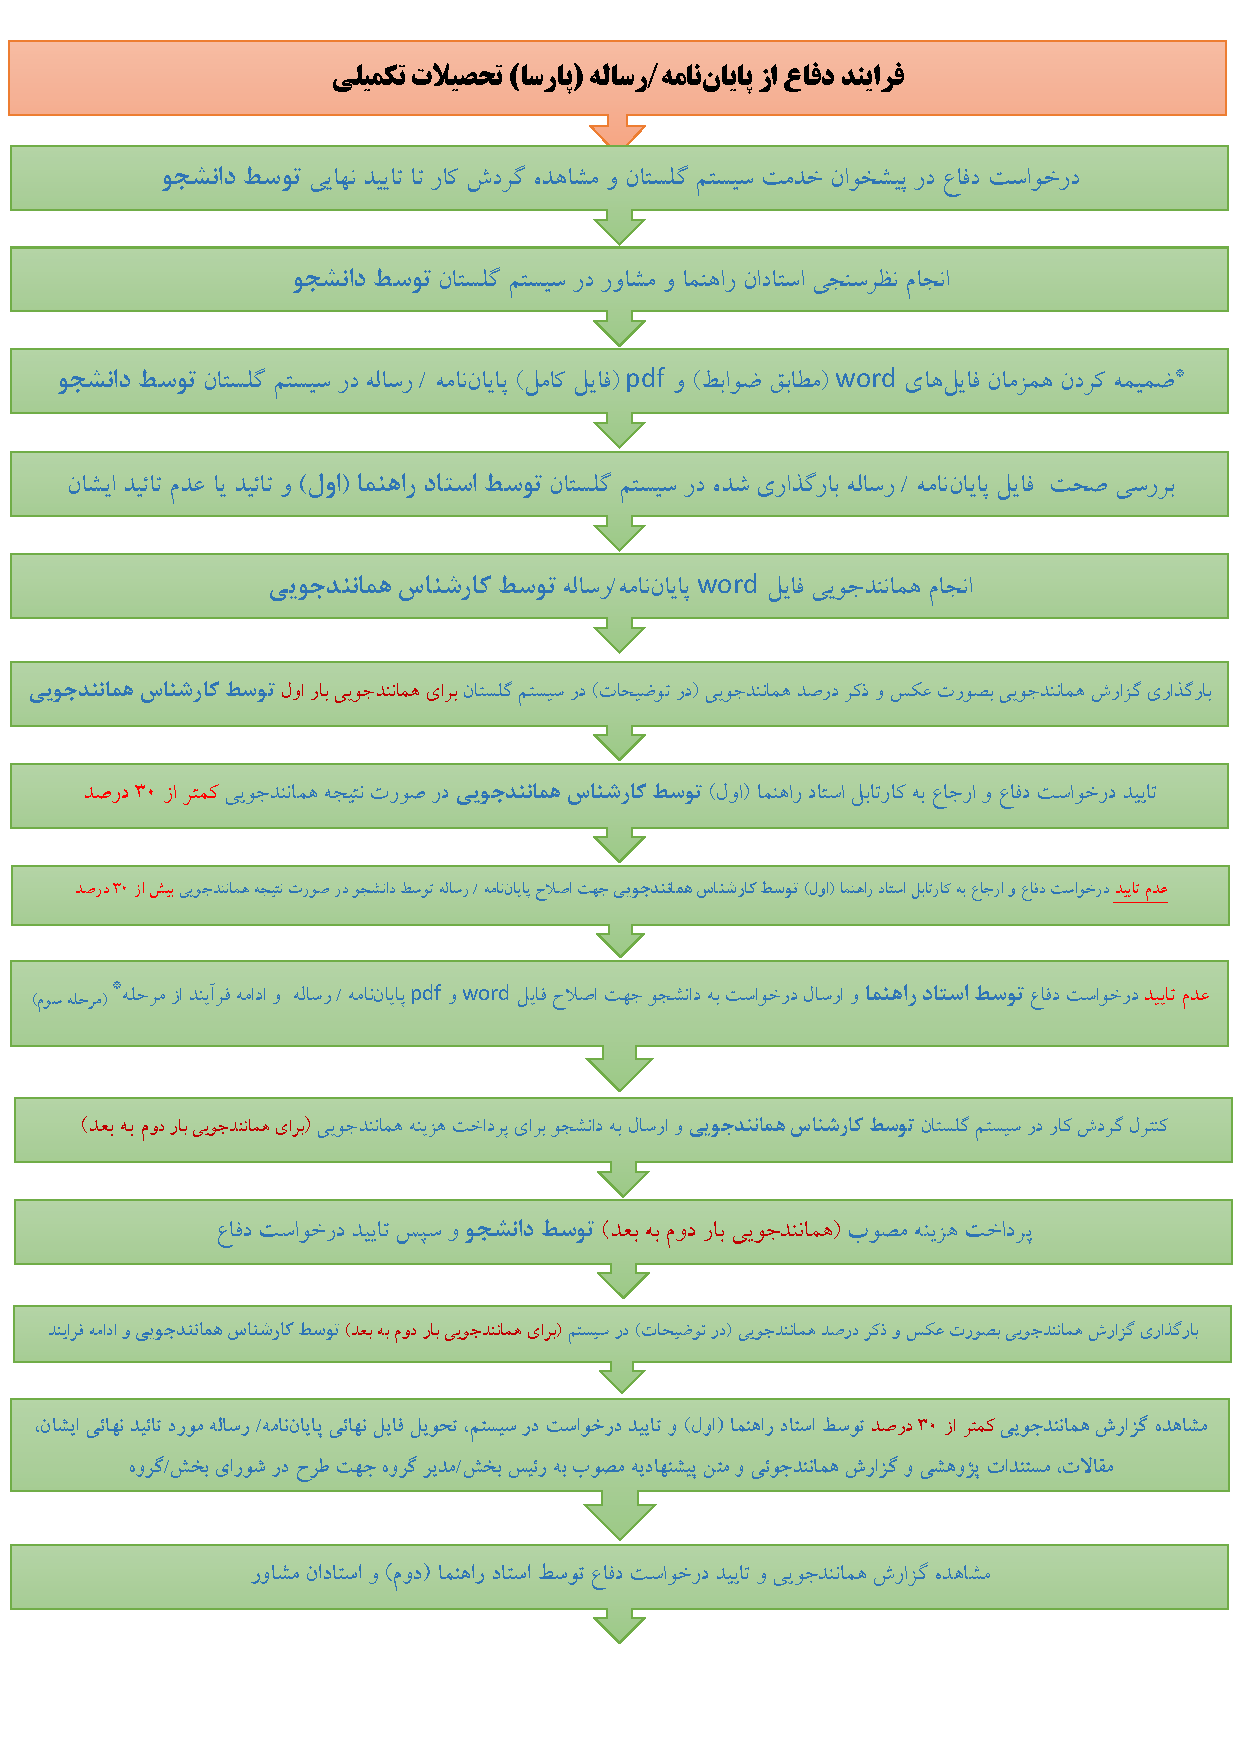
\includegraphics[width=0.95\textwidth]{defence-chart_Part1}}

\centerline{\includegraphics[width=\textwidth]{defence-chart_Part2}}

\section{توصیه‌های تحصیلات تکمیلی دانشگاه در خصوص پارساها}
این دستورالعمل به منظورآشنایی و آگاهی دانشجویان با نحوه نگارش و چگونگی تدوین و تنظیم مطالب یک تحقیق علمی (رساله) 
تهیه شده و ضروری است دانشجویان نکات مطرح شده در آن را هنگام تنظیم رساله رعایت نمایند.

\subsection{ بخش‌های رساله }

رساله باید مشتمل بر بخش‌های زیر باشد: 
\begin{enumerate}
\item شناسنامه یا صفحه عنوان (به زبان فارسی)
\item  شروع با ذکر نام خداوند
\item  صورت‌جلسه (فارسی) هیأت داوران جلسة دفاع از رساله 
\item  تعهدنامۀ رعایت حقوق معنوی دانشگاه یزد
\item  منشور اخلاق پژوهش
\item  تقدیم (اختیاری)
\item  سپاس و قدردانی (اختیاری)
\item  چکیده فارسی  
\item  فهرست مطالب
\item  فهرست شکل‌ها (در صورت داشتن شکل یا نمودار)
\item  فهرست جدول‌ها (در صورت داشتن جدول)
\item  فهرست نمادهای اختصاری و اختصارات (در صورت داشتن علائم، اختصارات و نمادهای اختصاری)
\item  پیشگفتار (اختیاری و با تصویب پردیس/دانشکده مستقل)
\item  متن اصلی که مشتمل بر فصل‌های مختلف از جمله مقدمه یا دیباچه، مروری بر منابع و مطالعات انجام شده و اهداف پژوهش، روش تحقیق، نتایج و تجزیه و تحلیل و تفسیر آنها، نتیجه‌گیری و پیشنهادها است. (مقدمه، فصل اول تلقی می‌شود.)
\item  واژه‌نامه فارسی به انگلیسی یا بالعکس (اختیاری و با تصویب پردیس/دانشکده مستقل و تایید شورای تحصیلات تکمیلی دانشگاه)
\item  فهرست منابع و مآخذ
\item  پیوست‌ها (در صورت وجود)
\item ABSTRACT (چکیده به زبان انگلیسی)
\item  شناسنامه یا صفحه عنوان (به زبان انگلیسی)
\end{enumerate}

\subsection{ حروف‌نگاری (تایپ) رساله}
\begin{enumerate}
 \item برای تایپ رساله از نرم‌افزار Word (نسخه 2013 یا بالاتر) یا LATEX استفاده شود و ترجیحاً متن اصلی با قلم 
BNazanin 14 (یا فونت مصوب پردیس/ دانشکده مستقل با تأیید شورای تحصیلات تکمیلی دانشگاه) باشد. 
متون انگلیسی با قلم \lr{Times New Roman 12} تایپ شود. برای تایپ رساله‌های رشتۀ ادبیات عرب ترجیحاً از قلم 
بدر عربی 15 استفاده شود.

\begin{center}
\begin{tabular}{|c|c|c|} \hline
نوع متن &	فونت فارسی	& فونت انگلیسی \\ \hline
متن عادی &	\lr{BNazanin 14}&	\lr{Times New Roman 12}\\ \hline
شماره صفحه‌ها	& \lr{BNazanin 12}	& \lr{Times New Roman 10}\\ \hline
عنوان فصل‌ها&	\lr{BNazanin Bold 18}	& \lr{Times New Roman Bold 16}\\ \hline
عنوان بخش‌ها	& \lr{BNazanin Bold 16}	& \lr{Times New Roman Bold 14}\\ \hline
عنوان زیربخش‌ها	& \lr{BNazanin Bold 14}	&\lr{Times New Roman Bold 12}\\ \hline
عنوان شکل‌ها/نمودارها و جدول‌ها	& \lr{BNazanin 12}	&\lr{Times New Roman 11}\\ \hline
سربرگ (Header) هر فصل &	\lr{BNazanin 12}	& \lr{Times New Roman 11}\\ \hline
\end{tabular}
\end{center}

\item  در صفحه‌های سمت چپ فایل رساله، فاصله شروع خط تا لبه راست صفحه 4 سانتیمتر -به غیر از سطر مطلع پاراگراف 
که تا لبه صفحه پنج سانتیمتر باشد. فاصله خط تا لبه بالای صفحه سه سانتیمتر، لبه پایین و لبه چپ صفحه 5/2 سانتیمتر باشد. 
در صفحه‌های سمت راست، فاصله شروع خط تا لبه راست صفحه 5/2 سانتیمتر ـ به‌غیر از سطر مطلع پاراگراف که تا لبه صفحه
 5/3 سانتیمتر باشد ـ فاصله خط تا لبه بالای صفحه سه سانتیمتر، لبه پایین صفحه 5/2 و لبه چپ 4 سانتیمتر باشد. 
 فاصله عنوان مطلب تا اولین سطر نوشـته شده 2 سانتیمتر و فاصله بین خطوط 1 سانتیمتر 
 (\lr{Line Spacing: Exactly 29 pt}) باشد. فاصله شماره صفحه از لبه پایین صفحه 1 سانتیمتر باشد. 
 این فواصل برای خطوط در تمام مراحل تدوین رساله اعم از شکل‌ها / نمودارها، جداول، فهرست، عکس‌ها و غیره باید رعایت شود.
\item  
 جدول‌هایی که در راستای طولی صفحه تنظیم می‌شوند، باید طوری قرار گیرند که متن بالای آنها در سمت عطف رساله واقع شود
 و همچنین شکل‌هایی که در راستای طولی صفحه تنظیم می‌شوند، باید طوری قرار گیرند که متن پایین آنها در سمت لبه 
 رساله قرار گیرد. شکل‌ها و جدول‌ها حتی‌المقدور داخل متن و در نزدیک‌ترین فاصله به محلی که ذکر شده، آورده شوند.

توجه: در تدوین و تایپ صفحه‌های رساله به غیر از صفحه‌های تقدیم و سپاسگزاری از هیچ‌گونه کادر تزئینی و تذهیب استفاده نگردد.
\item 
 سعی شود تا حد امکان از به کار بردن واژه‌های با الفبای انگلیسی در متن رساله فارسی خودداری شود و در صورت نیاز، 
معادل انگلیسی لغت‌ها، اصطلاح‌های فارسی یا افراد خاص به صورت پانویس در صفحه‌ مربوطه درج شود (فقط یک‌بار و 
در اولین بار استفاده از آن کلمه). 
پانویس‌ها زیر یک خط که به فاصله‌ 5/2 سانتیمتر از لبه چپ صفحه و حداقل 3 سانتیمتر از لبه پایینی و به طول مورد نیاز 
رسم می‌شود، نوشته شوند. (در هر صورت لازم است 5/2 سانتیمتر حاشیه پایین صفحه رعایت شود). پانویس‌ها در هر صفحه 
با گذاردن شماره 1، 2 و ... در گوشه‌ بالای انتهای کلمه در متن مشخص شوند. (در مورد اصطلاحات و عبارت‌های علمی، توصیه 
شود که تا حد امکان از معادل فارسی مناسب استفاده شود و در مورد اسامی افراد خارجی هم از روال یکسانی برای همه اسامی 
استفاده شود).
\item 
 در نگارش کلماتی نظیر آن‌ها و ... که از دو بخش تشکیل شده است ولی یک کلمه (یا مفهوم) محسوب می‌شود بایستی ارتباط 
بین دو بخش به‌صورت "جداکننده بدون فاصله" (فشردن کلیدهای Shift+Space بصورت همزمان در صفحه کلید استاندارد 
فارسی) رعایت شود.
\item 
 برای قرار دادن علائم نگارشی نظیر نقطه، ویرگول، علامت سوال، علامت تعجب و ... بایستی بین این علائم و کلمات قبل 
فاصله‌ای نباشد ولی بعد از آن یک فاصله ایجاد شود.
\item 
 در مورد پرانتز، بین عبارت‌های داخل پرانتز و پرانتز فاصله‌ای نباشد، اما بین پرانتزها و عبارت‌های دو طرف آن یک فاصله 
قرار گیرد.
\item 
 نوشتن کلماتی مانند به‌جز، به‌سرعت، به‌دقت و ... به‌صورت بجز، بسرعت، بدقت و ... اشتباه است و بایستی بصورت مجزا 
و با رعایت نیم‌فاصله نوشته شوند. برای اطلاع از جزئیات بیشتر می‌توان به منابعی نظیر "دستورخط فارسی"، "به‌نویسی" 
و... مراجعه کرد.
\item 
 علامت نقطه-ویرگول (؛) یا مکث میانه در مواردی استفاده می‌شود که مفهوم جمله ناتمام است.
\item 
 سعی شود از نوشتن پاراگراف‌های طولانی اجتناب شود. 
\item 
 توصیه می‌شود در انتهای هر فصل به‌جز فصل مقدمه، یک بخش جمع‌بندی یا خلاصه فصل وجود داشته باشد. (با تایید پردیس/ دانشکده مستقل).
\item 
 توصیه می‌گردد برای نوشتن فرمول‌ها و روابط ریاضی در نرم‌افزار Word، از افزونه یا نرم‌افزار Mathtype استفاده شود.
\item 
 فهرســت مطالب ارائه شده با توجه به قالب مورد تایید هر دانشکده/ گروه مستقل می‌تواند متفاوت از نمونه ذکر شده در این فایل باشد.
\item 
 توصیه می‌شود عنوان هر فصل بالای صفحات مربوط به آن فصل به‌صورت سربرگ (Header) آورده شود. 
\end{enumerate}
\subsection{ شماره‌گذاری}
\begin{enumerate}
\item  شماره‌گذاری صفحه‌ها

در هنگام شماره‌گذاری صفحه‌های رساله، موارد قبل از فهرست مطالب (موارد 1 الی 8 قسمت الف) هیچگونه شماره‌ای داده نشود. 
شماره‌گذاری فهرست‌ها و پیشگفتار با استفاده از حروف ابجد یا اعداد رومی انجام شود و شماره‌گذاری متن اصلی با استفاده از اعداد 
فارسی تا آخرین صفحه انجام شود. توجه گردد در صفحۀ اول هر فصل که عنوان فصل نوشته می‌شود، شماره‌ صفحه ذکر نشود، 
لیکن به حساب آید. شماره‌گذاری صفحه‌ها باید وسط و به فاصله 1 سانتیمتر از لبه پایین صفحه باشد.
\item 
 شماره‌ گذاری فصل‌ها، بخش‌ها و زیربخش‌ها

بخش‌ها و زیربخش‌های مختلف هر فصل با اعدادی نظیر 6-4 یا 6-4-2 مشخص می‌شود که عدد 6 شماره‌ فصل، عدد 4 شماره 
بخش و عدد 2 شماره قسمت است. شماره و عنوان هر فصل با قلم \lr{BNazanin 18 Bold} و عناوین بخش‌های مختلف 
هر فصل با قلم \lr{BNazanin 16 Bold} و عناوین قسمت‌های هر بخش با قلم \lr{BNazanin 14 Bold}
 تایپ شود (یا فونت‌های مصوب پردیس/ دانشکده مستقل و تأیید شورای تحصیلات تکمیلی دانشگاه). ضمناً عناوین فصل‌ها 
 و بخش‌های زیر فصل حتماً به صورت خودکار با استفاده از levelهای word تنظیم گردند.
\item 
 شماره‌ گذاری جدول‌ها، شکل‌ها 

برای شماره‌گذاری جدول‌ها و شکل‌ها در متن اصلی رساله از دو شماره که با خط فاصله از یکدیگر جدا می‌گردند، استفاده 
می‌شود به‌طوری‌که تمام جدول‌ها و شکل‌ها از ابتدا تا انتهای رساله به ترتیب دارای شماره 1، 2، ... و n برای هر فصل خواهند 
بود که شماره سمت چپ نشان‌دهنده ترتیب جدول / شکل و شماره سمت راست نشان‌دهنده شماره فصلی است که جدول / شکل 
در آن ذکر گردیده است. (مثلاً برای فصل 2: جدول 2-1، جدول 2-2 و ...، برای فصل 3: جدول 3-1، جدول 3-2 و ...). شماره‌گذاری 
جدول-ها، شکل‌ها و.... مستقل از همدیگر صورت می‌گیرد (البته قابل ذکر است که «نمودار»ها هم جزء «شکل»ها تلقی می شوند و نیاز
 به تیتر (عنوان) مجزایی ندارند). عنوان جدول‌ها در بالای آنها و عنوان شکل‌ها در زیر آنها ذکر می‌گردد.
شماره‌ای که در متن به شکل‌ها، جدول‌ها و ... اختصاص داده می‌شود، باید به همان صورت، در فهرست جدول‌ها، شکل‌ها و ... 
که قبل از شروع متن اصلی در رساله تنظیم می‌گردد، ذکر شود. فهرست مطالب، فهرست شکل‌ها و فهرست جدول‌ها و... به 
صورت خودکار در word ایجاد شود.
\item 
 شماره ‌گذاری روابط و فرمول‌ها

 فرمول‌ها در هر فصل به طور جداگانه و به ترتیبی که ظاهر می‌شوند (مانند جدول‌ها و شکل‌ها)، شماره‌گذاری گردد. 
 شماره‌گذاری روابط و فرمول‌های نوشته شده در متن اصلی رساله مشابه با جدول‌ها و شکل‌ها از ابتدا تا انتهای رساله به 
 ترتیب 1، 2، ... و n برای هر فصل و در پرانتز لحاظ خواهند شد. به‌طور مثال فرمول بیستم در فصل سوم به‌صورت (3-20) 
 نوشته می‌شود.
در مورد شماره‌گذاری قضیه‌ها، گزاره‌ها، لم‌ها، مثال‌ها و نظایر آنها در هر فصل به‌طور جداگانه و به-ترتیبی که در متن می‌آیند 
شماره‌گذاری می‌شوند؛ این شماره‌گذاری چنان است که شماره فصل در سمت راست و شماره قضیه (و نظایر آن) بعد از آن آورده
 شده و بین آنها از نقطه استفاده می‌شود. لازم است کلمه قضیه (و نظایر آن) و شماره آنها به صورت قلم سیاه (Bold) نوشته شده
 و پس از آن علامت دو نقطه (:) آورده شود. همچنین برای شروع اثبات کلمه اثبات همراه (:) به صورت قلم سیاه می‌آید؛ (معمولا 
 برای رشته‌های دانشکده علوم ریاضی و ...)
\end{enumerate}
\subsection{منابع و مآخذ}

لازم است در متن به کلیه منابعی که مورد استفاده قرار می‌گیرد، اشاره شود. مرجع دهی باید بر اساس قالب مورد تصویب 
دانشکده / گروه مستقل باشد و اگر دانشکده / گروه مستقل قالب خاصی را تعیین نکرده، از قالب APA استفاده شود.
در صورتی‌که از نرم‌افزار مدیریت مرجع استفاده نمی‌شود معمولا به یکی از دو روش زیر در متن به مراجع اشاره می‌گردد:

\begin{enumerate}
\item  مراجع به ترتیبی که در متن می‌آیند شماره‌گذاری شوند. در این روش، مراجع به ترتیب شماره در فهرست 
منابع و مآخذ ذکر گردد. 
\item 
مراجع به ترتیب حروف الفبایی نام خانوادگی نویسنده اول شماره‌گذاری گردیده، به همین ترتیب در فهرست منابع و مآخذ 
ذکر می‌شود.
القاب و عناوین دکتر، مهندس و … از جلوی نام مؤلف، مترجم حذف می‌گردد و همچنین اگر کتاب دارای دو نویسنده یا 
بیشتر باشد نام و نام خانوادگی همه آنها به ترتیبی که در روی جلد کتاب آمده است، آورده شود.

به‌طور مثال:

یاحقی، محمد جعفر و ناصح، محمد مهدی، راهنمای نگارش و ویرایش، چاپ هشتم، مشهد: آستان قدس رضوی، ص106.

در صورت وجود منابع به زبان‌های مختلف، توصیه‌ می‌شود مراجع غیرانگلیسی نیز به انگلیسی ترجمه و در 
انتها واژه‌ی (\lr{in Persian}) داخل پرانتز قید شده و سال آنها نیز به میلادی برگردان شوند. در غیر این صورت، 
ابتدا مراجع فارسی و سپس سایر مراجع ذکر شود. 
اگر شکل یا جدولی از منبع و مأخذی گرفته شده، لازم است مرجع آن در انتهای عنوان آن شکل یا جدول آورده شود.
\end{enumerate}
\subsection{شیوه‌نامه پردیس فنی و مهندسی}
برای دانشجویان پردیس فنی و مهندسی رعایت موارد ذیل الزامی است.
\begin{enumerate}
\item  استفاده از نرم‌افزار مدیریت مرجع مانندEndnote ، Mendeley و ... الزامی است.
\item  برای ارجاع بصورت شماره از قالب IEEE  و برای ارجاع با استفاد از نام و تاریخ از قالب APA استفاده شود.
\item  در صورت وجود منابع به زبان‌های مختلف، ضروری است مراجع غیرانگلیسی نیز به انگلیسی ترجمه و در انتها واژه‌ی
 (in Persian) داخل پرانتز قید شده و سال آنها نیز به میلادی برگردان شوند.
\end{enumerate}
\section{آماده‌سازی فایل جهت همانندجویی}
با توجه به نیاز به همانندجویی پیشنهادیه و پارساهای دانشگاه، لازم است کلیه دانشجویان در زمان درخواست دفاع با تصویب پیشنهادیه، 
فایل پیشنهادیه/پایان‌نامه با فرمت Word را در سامانه گلستان بارگذاری نمایند تا همانندجویی روی آن‌ها  انجام شود. 

برای دانشجویانی که از زیپرشن برای تایپ پایان‌نامه استفاده کرده‌اند، کافی است محتویات فایل \lr{.tex} را که محتوای پایان‌نامه آنها است را به 
همان صورت کپی و در یک فایل Word الصاق نمایند و فایل Word حاصل را برای همانندجویی بارگذاری دهند. لازم به ذکر است که نیاز به 
صفحات اولیه و مراجع پیشنهادیه/پایان‌نامه برای همانندجویی نیست.
 
راهکار دیگری که پیشنهاد می‌شود و البته مستلزم استفاده از ابزاری به نام GrindEQ است، این است که با نصب این ابزار، فایل اصلی پیشنهادیه/پایان‌نامه 
را در Word باز نمایید تا تمام پایان‌نامه به Word تبدل شود. البته این ابزار مجانی نیست، ولی برای هر نصب، تا 10 تبدیل را انجام می‌دهد. 
با این تبدیل، تمام فرمول‌ها و غیره کاملا منتقل می‌شود. تنها مشکل آن، نداشتن ساختار است و شکل‌ها نیز بعضا منتقل نمی‌شود که می‌شود دستی اصلاح 
کرد. البته برای همانندجویی، نیازی به داشتن شکلها نیست. راهنمای نصب و استفاده از این ابزار در بخش~\label{sec:grineq} آمده است.

%\newpage 
\subsection{ دستورالعمل ورود اطلاعات پایان‌نامه کارشناسی ارشد/ رساله دکتری توسط دانشجو در سامانه \lr{Irandoc}}
% پژوهشگاه علوم و اطلاعات ایران (Irandoc)}

\centerline{\includegraphics[width=0.6\textwidth]{Irandoc}}
\pagebreak 

\subsection{برخی نکات نگارشی}
در نوشتن مطالب علمی، رعایت قوانین نگارشی لازم است. در این کوتاه، صرفاً به برخی نکات نگارشی مهم اشاره می‌شود که لازم است در متن
پارساها به آن‌ها توجه شود. لازم به ذکر است که در خصوص برخی از قوانین نگارشی، ممکن است اختلاف نظری وجود داشته باشد ولی اکثر موارد 
ذکرشده مورد اتفاق است.
\begin{enumerate}
\item  علائم سجاوندی مانند کاما، ؛، .، :، ! و ؟ بدون فاصله با کلمه‌ی قبل از خود نوشته می‌شوند، ولی بعد از
آن‌ها باید یک فاصله‌ی خالی قرار گیرد. مانند: من، تو؛ او.
\item 
 علامت‌های پرانتز، آکولاد، کروشه، نقل‌قول و نظایر آن‌ها، بدون فاصله با عبارت داخل خود نوشته 
می‌شوند، ولی با عبارت اطراف خود یک فاصله دارند. مانند: (اين)،  (آن) و «آن‌ها».
\item 
  علامت استمرار «می» جدای از کلمه‌ی بعد خود و بی‌فاصله با آن (یعنی با نیم‌فاصله) نوشته می‌شود. مانند: می‌دهیم، می‌شود.
\item 
 علامت جمع «ها»، علامت صفت برتری «تر» و علامت صفت برترین «ترین»؛ جدای از کلمه‌ی قبل از خود و بی‌فاصله با آن  (یعنی با نیم‌فاصله) نوشته می‌شود. 
 مانند: آن‌ها بیش‌تر و کم‌ترین.
 
تبصره: کلمه‌های بهتر و بهترین از این قاعده مستثنا هستند.
\item 
 شناسه‌های «ام». «ایم»» «ای». «اید» و «اند» بی‌فاصله با کلمه‌ی قبل از خود  (یعنی با نیم‌فاصله) نوشته می‌شوند. ولی «است» با
فاصله است، مگر وقتی که کلمه‌ی قبلی با «ه» یا «ا» تمام شود. مانند: رفته‌ام رفته است. از ماست که برماست.
\item 
 ضمیرهای متصل جمع جدا ولی بدون فاصله با کلمه‌ی قبل خود  (یعنی با نیم‌فاصله) نوشته می‌شوند. مانند: زندگی‌مان؛
راه‌شان» ولی ضمیرهای متصل مفرد متصل نوشته می‌شوند. مانند: راهم نامت و کتابش.
\item 
 «به» هميشه جدا از کلمه‌ی قبل از خود ولی بدون فاصله  (یعنی با نیم‌فاصله) نوشته می‌شود. مگر در مواری که فعل ساخته
شود. مانند: به‌نام، به‌سزا، ببینیم.
\item 
 «به» هم‌واره جدا از کلمه‌ی قبل از خود ولی بدون فاصله نوشته می‌شود. مگر در مواری که حرف
اضافه‌ی «به» به تنهایی به‌کار رفته باشد. مانند: به‌سوی, به‌طرف، به آن‌ها.
\item 
‏ اجزای فعل با فاصله نوشته می‌شوند، مگر وقتی که یک جزء آن حرف اضافه باشد که در آن ‌صورت؛
حرف اضافه با کلمه‌ی بعد فاصله نخواهد داشت. مانند: تحریر کردن، درآورده شد، برآمده است، به‌کار
‏گرفتن.
\item 
 پیشوندها و پسوندهای جامد سرهم نوشته می‌شوند. مانند: دانشگاه، همسایه، همسر.
 
تبصره: در مورادی که خواندن کلمه دچار اشکال شود، می‌توان پسوند و پیشوند را جدا کرد. مانند: هم‌میهن، هم‌ارزی.
\item 
 اجزای حروف اضافه‌ی مرکب، قیدها، اسم‌ها، و صفت‌های مرکب بی‌فاصله نوشته می‌شوند. مانند: دراین‌صورت، آن‌گاه، به‌طوری‌که، کتاب‌خانه، دانش‌جو.
 \item 
 کلمه‌های مرکب دیگر نیز جدا و بدون فاصله نوشته می‌شوند. مانند: گفت‌وگو، پرس‌وجو و جست‌وجو.
 \item 
به‌دلیل دشواری خواندن، می‌توان «ها»ی ملفوظ را از قوانین جداسازی استثنا نمود. مانند: راهنما؛ رهبر.
\item 
 کسره‌ی اضافه‌ی بعد از «ه» به‌صورت «ه‌ی» نوشته می‌شود، نه «ۀ». مانند: خانه‌ی علی.
 
تبصره: اگر «ه» ملفوظ باشد. نباید «ی» را نوشت. مانند: فرمانده کل، پادشه خوبان.
\item 
 پایه‌های همزه در کلمه‌ها همیشه «ئ» است. مگر در مواری که همزه ساکن باشد. که دراین‌صورت باید
متناسب با اعراب حرف قبل نوشته شود. مانند: مسئله، مسئول، رأس، مؤمن.

تذکر: همزه‌ی بعد از حرف کشیده‌ی «ا» نوشته نمی‌شود. مانند: املا، استقرا، استثنا.
\item 
سعی شود جمع‌های کلمه‌های عربی به فارسی نوشته شود. مانند: شکل‌ها (به‌جای اشکال)، عبارت‌ها (به‌جای عبارات)، علامت‌ها (به‌جای علائم).
\item 
 جملات نقل‌قول یا موکد درون علامت نقل‌قول « و » قرار می‌گیرند. نه بین " *. مانند «استعداد خوب».
\item 
کلمه‌هایی که با جدانویسی خواناترند. جدا و بدون فاصله نوشته می‌شوند. مانند: چه‌گونه (به‌جای چگونه).
\item 
 «ی» عربی به‌صورت «» نوشته می‌شود. مگر آن‌که خوانند دچار مشکل شود. مانند: حتا و مستثنا.
 \item در کلمه‌های دو بخشی که به همراه هم یک مفهوم را مشخص می‌کنند، از نیم فاصله استفاده شود. مانند خوشه‌بندی، بهینه‌سازی، پیاده‌سازی و پایان‌نامه.
 یک راه  تشخیص، نگاه به کلمه انگلیسی معادل است. مثلاً \lr{clustering}  و \lr{optimization} و \linebreak 
 \lr{implementation} و \lr{thesis}.
 \item در استفاده از کاما برای روان‌تر شدن خواندن جملات استفاده شود. معمولاً هر جا در خواندن جمله یک توقف کوتاه رخ می‌دهد، باید کاما اضافه‌ شود.
 مانند «همچنان که در بخش قبل بیان شد، الگوریتم‌های ابتکاری کاربرد بسیاری در ....»
 \item حتی‌الامکان از معادل فارسی کلمات انگلیسی استفاده شود. مانند روش به جای تکنیک.
\end{enumerate}

\section{چند راهکار ساده اما راهگشا!}
یکی از وقت‌گیرترین کارهای آماده‌سازی یک متن علمی، مخصوصاً  در تجربه‌های اول، وفور خطاهای عمدتاً نگارشی است
که رفع آن‌ها، اولاً وقت زیادی می‌گیرد و ثانیاً نیاز به تمرکز بسیار دارد و حقیقتاً حوصله دانشجویان را به سر می‌برد. در این فصل راهکارهای ساده‌ای
ارائه می‌شود که می‌توانید این روند را سریع و بدون دردسر و با دقت زیاد انجام دهید.

\subsubsection{راهکار اول: از replace استقاده کنید!}
فرض کنید در پایان‌نامه، کلمه «می شود» را به همین صورت اشتباه استفاده کرده‌اید. لذا باید همه موارد استفاده شده به صورت «می شود» را به «می‌شود»
اصلاح نمایید. انجام این کار به صورت دستی و مورد به مورد بسیار مشکل است و در نهایت نیز مواردی از چشم شما پنهان می‌ماند. اما با استفاده از امکان
replace که تقریباً در تمام ادیتورها در دسترس هستند، می‌توانید این کار را در سرتاسر پایان‌نامه با صرف چند دقیقه و بدون نیاز به بررسی چشمی
انجام دهید. برای این کار replace ادیتور خود را انتخاب کنید (این کار در \lr{Notepad++} با کلید میانبر \lr{CTRL+H} می‌توانید انجام دهید).
سپس در قسمت \lr{Find}،  کلمه «می شود» و در قسمت \lr{Replace with}، کلمه «می‌شود» (هر دو بدون گیومه اول و آخر) قرار دهید. سپس گزینۀ
\lr{Find} را کلیک کنید و کلمه «می شود» بعدی را ببینید و اگر مایل به جایگزین هستید، گزینه \lr{Replace} را انخاب کنید. تکرار انتخاب ترتیبی
گزینه‌های \lr{Find} و \lr{Replace} به ترتیب اشکالات را پیدا و رفع می‌نماید. این کار را در تمام فایل‌های مربوط به پایان‌نامه خود تکرار کنید. اگر
از عدم وجود ترکیب‌های مشابه اطمینان دارید، می‌توانید با انتخاب گزینۀ \lr{Replace All}، همه اصلاحات را بدون چک کردن انجام دهید ولی برای 
استفاده از این گزینه دقت کنید زیرا ممکن است ترکیب مورد نظر شما در کلمات دیگری هم باشد که مایل به تغییر آن‌ها نباشید.

\subsubsection{راهکار دوم: استفاده از \lr{Inverse-Search}}
یکی از مشکلات کار با لاتک در مقایسه با \lr{Word} این است که متن نهایی با  متن نوشته شده متفاوت است. لذا اگر جایی از متن نیاز به
اصلاح داشته باشد، باید محل متناظر را در فایل tex یافت و سپس آن را اصلاح کرد. این کار، مخصوصاً اگر سند ما مفصل و چند ده صفحه‌ای باشد، بسیار
وقت‌گیر و خسته کننده است. اما اگر از \lr{SumatraPDF} استفاده کنید و نام پوشه و ابرپوشه‌های حاوی فایل سند شما فارسی نباشد، به راحتی با 
دوبار کلیک روی هر محل در فایل پی دی اف که در نرم‌افزار \lr{SumatraPDF} باز شده است، به محدوده همان محل در فایل tex مربوطه
منتقل می‌شوید. با این کار، عملاً نیاز به جستجوی طولانی مدت برای پیدا کردن محل ندارید.

\subsubsection{راهکار سوم: خطایابی و رفع خطا در بازه‌های زمانی کوتاه}
همانطور که در فیلم‌های آموزشی دوره مقدماتی لاتک آمده است، لاتک اصولاً یک زبان برنامه‌نویسی است که برای حروف‌چینی متون است. لذا، مشابه
یک برنامه، در صورت رعایت نشدن فرمت دستورات آن، در زمان حروف‌چینی با خطا مواجه خواهید شد. این خطا ممکن است به دلایلی نظیر
فراموش شدن یک علامت $\$$ یا  $\}$ باشد. البته، لاتک در صورت بروز خطا، تا بتواند کار را انجام می‌دهد اما اگر خطا به گونه‌ای باشد که کل کار را
مختل نماید، ممکن است بخشی یا کل متن حروف‌چینی نشود و در فایل پی دی اف نهایی نیاید. همانطور که در برنامه‌نویسی توصیه می‌شود، توصیه این است
که در زمان تایپ متن، در دوره‌های کوتاه‌مدت، متن را حروف‌چینی کنید و در صورت بروز خطا، آن را برطرف نمایید و پس از برطرف کردن کامل
خطاها، تایپ بخش بعدی را شروع نمایید. با این کار محدوده شما برای خطایابی کوچک بوده و معمولاً خطاها به سرعت پیدا و اصلاح می‌شوند.
\subsubsection{راهکار چهارم: گرفتن منظم نسخۀ پشتیبان}
هرچند فایل‌های لاتک، متنی هستند و مشابه فایل‌های ابزارهای مثل \lr{Word} نیستند که خراب شوند، ولی حذف شدن فایل یا رونویسی شدن
آن‌ها می‌تواند باعث از دست رفتن بخشی از کار شود. لذا توصیه کلی این است که نسبت به نسخه پشتیبان گرفتن از فایل‌های خود به طور منظم و در فواصل
نه چندان طولانی اقدام نمایید. همچنین می‌توانید ادیتور مورد استفاده خود را بررسی کنید و در صورت داشتن امکانات ایجاد فایل‌های پشتیبان به صورت
خودکار، آن را فعال نمایید.!
داخل فایل
\LRE{\verb!yazd-thesis-template.tex!}
و بعد از دستور
\verb!\chapter{راهنمای استفاده از کلاس \lr{yazd-thesis}}
\section{مقدمه}
حروف‌چینی پایان‌نامه یا رساله یکی از موارد پرکاربرد استفاده از زی‌پرشین است. از طرفی، یک  پایان‌نامه یا رساله،  احتیاج به تنظیمات زیادی از نظر صفحه‌آرایی  دارد که ممکن است برای
یک کاربر مبتدی، مشکل باشد. به همین خاطر، برای راحتی کار کاربر، کلاس حاضر با نام 
 \LRE{\verb!yazd-thesis!}
 برای حروف‌چینی پروژه‌ها، پایان‌نامه‌ها و رساله‌های دانشگاه یزد با استفاده از نرم‌افزار زی‌پرشین،  آماده شده است. این فایل به 
گونه‌ای طراحی شده است که کلیه خواسته‌های مورد نیاز  مدیریت تحصیلات تکمیلی دانشگاه یزد را برآورده می‌کند. همچنین حروف‌چینی بسیاری
از قسمت‌های آن، به طور خودکار انجام می‌شود.

کلیه فایل‌های لازم برای حروف‌چینی با کلاس گفته شده، داخل پوشه‌ای به نام
 \LRE{\verb!yazd-thesis!}
  قرار داده شده است. توجه داشته باشید که برای استفاده از این کلاس باید فونت‌های \lr{Yas}، \lr{Times New Roman}، 
  \lr{B Nazanin}  و \lr{Titr} روی کامپیوتر شما نصب باشد. این فونت‌ها در بین فونت‌های مشخص شده جهت نصب وجود دارد، ولی با توجه به این که
  ممکن است نصب \TeX{}Live از طریق دیگری انجام شده باشد، فونت‌های لازم در مسیر Fonts قرار گرفته است. می‌توانید این فونت‌ها را روی سیستم‌عامل
  خود نصب نمایید. تاکید می‌شود، در صورت نصب فونت، اگر با پیام وجود فونت روی کامپیوتر خود مواجه شدید، گزینه رونویسی فونت را انتخاب کنید تا از
  استفاده از نگارش مناسب فونت‌ها اطمینان حاصل نمایید.
 
\section{این همه فایل؟!}\label{sec2}
از آنجایی که یک پایان‌نامه یا رساله، یک نوشته بلند محسوب می‌شود، لذا اگر همه تنظیمات و مطالب پایان‌نامه را داخل یک فایل قرار بدهیم، باعث شلوغی
و سردرگمی می‌شود. به همین خاطر، قسمت‌های مختلف پایان‌نامه یا رساله  داخل فایل‌های جداگانه قرار گرفته است. مثلاً تنظیمات  کلاس داخل فایل
\LRE{\verb!yazd-thesis.cls!}، 
قسمت مشخصات فارسی پایان‌نامه داخل 
\LRE{\verb!fainfo.tex!}،
مطالب فصل اول، داخل 
\verb!chapter1!
و ... قرار داده شده است. نکته مهمی که در اینجا وجود دارد این است که از بین این  فایل‌ها، فقط فایل 
\LRE{\verb!yazd-thesis-template.tex!}
قابل اجرا است. یعنی بعد از تغییر فایل‌های دیگر، برای دیدن نتیجه تغییرات، باید این فایل را اجرا کرد. بقیه فایل‌ها به این فایل، کمک می‌کنند تا بتوانیم خروجی کار را ببینیم. اگر به فایل 
\LRE{\verb!yazd-thesis-template.tex!}
دقت کنید، متوجه می‌شوید که قسمت‌های مختلف پایان‌نامه، توسط دستورهایی مانند 
\verb!input!
و
\verb!include!
به فایل اصلی، یعنی 
\LRE{\verb!yazd-thesis-template.tex!}
معرفی شده‌اند. بنابراین، فایلی که همیشه با آن سروکار داریم، فایل 
\LRE{\verb!yazd-thesis-template.tex!}
است.
در این فایل، فرض شده است که پایان‌نامه یا رساله، از ۳ فصل و یک پیوست، تشکیل شده است. با این حال، اگر
  پایان‌نامه یا رساله، بیشتر از ۳ فصل و یک پیوست است، باید خودتان فصل‌های بیشتر را به این فایل، اضافه کنید. این کار، بسیار ساده است. فرض کنید بخواهید یک فصل دیگر هم به پایان‌نامه، اضافه کنید. برای این کار، کافی است یک فایل با نام 
\verb!chapter4!
و با پسوند 
\verb!.tex!
بسازید و آن را داخل پوشه 
\LRE{\verb!yazd-thesis!}
قرار دهید و سپس این فایل را با دستور 
\verb!\chapter[برخی نکات مفید]{ برخی نکات مفید ( اضافه کردن عنوان برای بیش از یک خط شدن)}
\twocolumnfootnotes
\section{فرایند تصویب پیشنهادیۀ پارسای تحصیلات تکمیلی}
در این بخش، فرآیند تصویب پیشنهادیۀ پایان‌نامه/رساله آورده شده است. 
دستورالعمل کامل مراحل تصویب و ثبت پیشنهادیۀ پایان‌نامه/ رساله دانشجویان تحصیلات تکمیلی در پیوست~\ref{ch:proposal}
آمده است.

لطفا برای مشاهده آخرین تغییرات به وبسایت تحصیلات تکمیلی دانشگاه به آدرس

\centerline{\url{https://yazd.ac.ir/offices/educational/deputy/graduate/home/rules}}

مراجعه نمایید.

\centerline{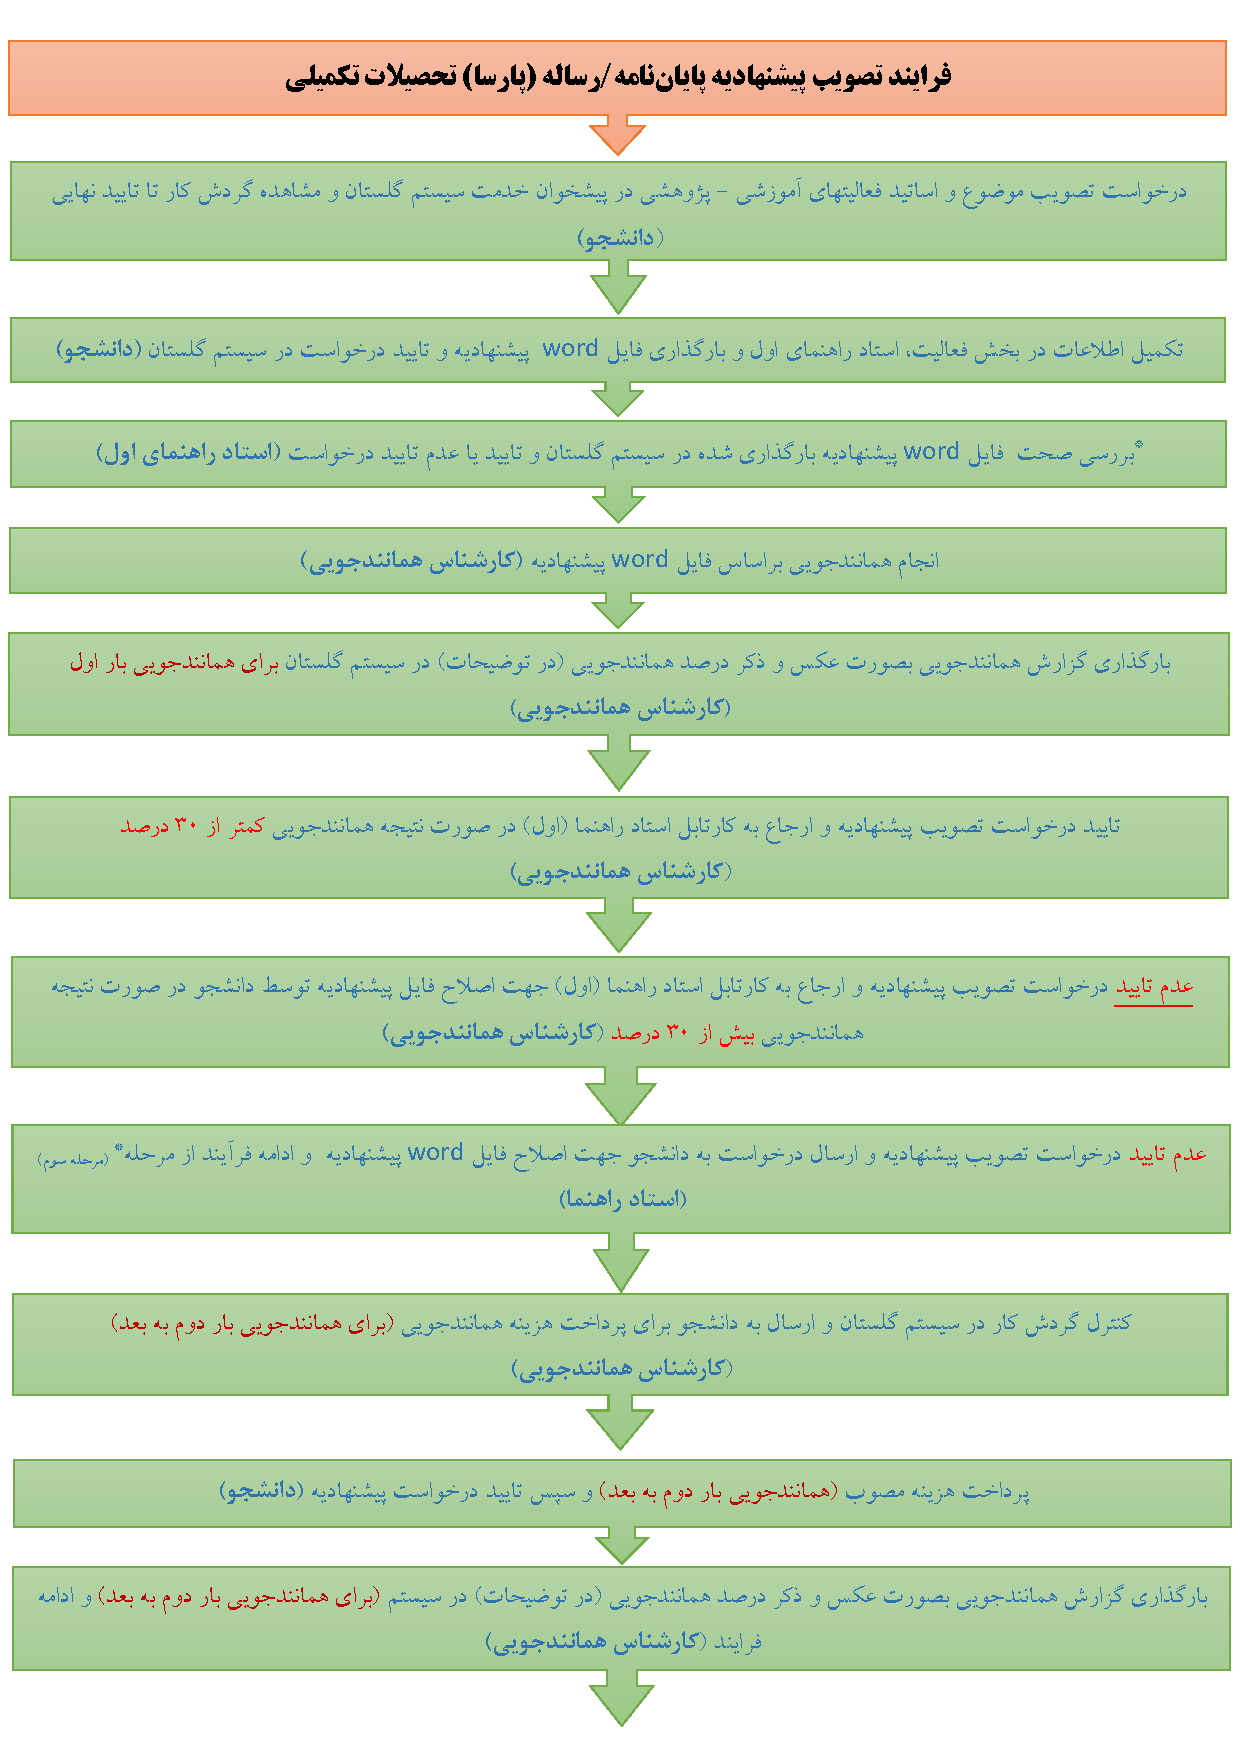
\includegraphics[width=0.9\textwidth]{Proposal-chart_Part1}}

\centerline{\includegraphics[width=\textwidth]{Proposal-chart_Part2}}

\section{دستورالعمل نحوه برگزاری جلسات دفاع }
\subsection{هدف }
هدف از تدوین این دستورالعمل ایجاد نظم و ترتیب بیشتر و شفاف‌سازی چگونگی برگزاری جلسات دفاع پایان‌نامه 
کارشناسی ارشد و رساله دکتری  و یادآوری نکات مهم برای برگزاری جلسه مطابق مقررات و شیوه‌نامه‌های تحصیلات تکمیلی‌است 
که بر اساس صورتجلسه شورای تحصیلات تکمیلی دانشگاه مورخ 17/2/1397 توسط نماینده تحصیلات تکمیلی (ناظر جلسه دفاعیه) 
دانشگاه مدیریت می‌گردد. 

\subsection{الف) فرآیند دفاع از پایان‌نامه / رساله }

\begin{enumerate}
\item  دانشجو: درخواست دفاع در پیشخوان خدمت

دانشجو در این قسمت ضمن درخواست دفاع‏، تاریخ و محل پیشنهادی دفاع از پایان‌نامه / رساله را بر اساس هماهنگی به عمل آمده
 با استادان راهنما / مشاور و پس از تایید اولیه رئیس بخش/ مدیرگروه ثبت می‌نماید. 
برای این منظور لازم است: 

*‌ دانشجو ظرف 48 ساعت، پایان‌نامه / رساله خود را همراه با مقالات مستخرج و تأییدیه‌های مجلات برای طرح در شورا به
 رئیس بخش / مدیرگروه تحویل و پس از تصویب جزئیات دفاع در شورا، فایل پایان‌نامه / رساله تصحیح شده نهایی و دستاوردهای
 مستخرج از آن را برای كارشناس تحصیلات تكمیلی ارسال کرده و فرآیند دفاع را تا مرحله تأیید معاون دانشكده / مدیرگروه مستقل پیگیری می‌نماید. 
 
*‌ برای دانشجویان دکتری لازم است كاربرگ بررسی مقالات از قبل با رعایت ضوابط مربوط تأیید و جلسه پیش دفاع دانشجو
 (حداقل 21 روز قبل از تاریخ دفاع) مطابق مقررات به طور موفقیت‌آمیز برگزار شده باشد و کاربرگ‌های مربوطه تکمیل، تایید و 
 به کارشناس جهت ثبت و بارگذاری در سیستم گلستان تحویل شده باشد.

\item  دانشجو: انجام نظرسنجی 

در این مرحله دانشجو باید نظرسنجی از استادان راهنما و مشاور پایان‌نامه / رساله را انجام و تایید نماید. 

\item  دانشجو: ضمیمه کردن همزمان فایل‌های word و  pdfپایان‌نامه / رساله

در این مرحله دانشجو فایل تصحیح شده نهایی پایان‌نامه / رساله را پیوست و برای انجام فرآیند همانندجویی ارسال می‌نماید. 
لازم به ذکر است فایل pdf  ضمیمه شده همان فایلی است که در اختیار اعضای هیأت داوران قرار می‌گیرد. 

* ضروری است تنها در نسخه word پایان نامه مفاد دستورالعمل بارگذاری رساله/پایان نامه برای همانندجویی رعایت شده باشد.

* هزینه همانندجویی برای مرحله اول به عهده دانشگاه و در سایر مراحل به عهده دانشجو است. 

\item  استاد راهنما: بررسی صحت  فایل پایان‌نامه / رساله بارگذاری شده 

در این مرحله استاد راهنما (اول) فایل پایان‌نامه / رساله بارگذاری شده توسط دانشجو را مشاهده، کنترل و در صورت عدم مغایرت، 
درخواست دفاع را تایید می‌نماید، در غیر اینصورت بایستی با انتخاب گزینه «عدم تایید» درخواست دفاع به کارتابل دانشجو عودت شود
 و دانشجو نسبت به انجام اصلاحات و بارگذاری فایل صحیح پایان‌نامه / رساله مجدداً اقدام نماید. 

\item  کارشناس همانندجویی دانشکده / گروه مستقل: انجام همانندجویی 

5-1- همانندجویی برای بار اول

کارشناس همانندجویی دانشکده / گروه مستقل، متن فایل word پیوست شده توسط دانشجو را در سامانه همانندجویی کپی 
و ارسال و نتیجه را در فایل دانشجو بارگذاری و درخواست را (با ذکر درصد همانندی در توضیحات) تایید / عدم تایید می‌نماید. 
*در صورتی که نتیجه همانندجویی کمتر از 30 درصد باشد، درخواست دفاع دانشجو تایید و به کارتابل استاد راهنما جهت طی 
مراحل بعدی ارجاع می‌شود. 

*در صورتی که نتیجه همانندجویی بیشتر از 30 درصد باشد، درخواست دفاع دانشجو عدم تایید و جهت اصلاح پایان‌نامه / رساله توسط دانشجو، 
به کارتابل استاد راهنما برمی‌گردد. 

5-2- همانندجویی برای بار دوم به بعد

*در صورتی که همانندجویی برای بار دوم به بعد انجام می‌شود (با کنترل گردش کار در گلستان)، کارشناس درخواست دفاع را برای 
پرداخت هزینه همانندجویی به دانشجو ارسال می‌‌نماید. 

5-2-1- دانشجو: پرداخت هزینه همانندجویی بار دوم به بعد

در صورتی که همانندجویی برای بار دوم به بعد انجام می‌شود دانشجو ملزم به پرداخت هزینه مصوب و تایید درخواست دفاع است. 

5-2-2- کارشناس همانندجویی دانشکده / گروه مستقل

 بعد از پرداخت هزینه توسط دانشجو فرآیند همانندجویی مطابق  بخش 5-1- انجام و ادامه می‌یابد. 

\item  استاد راهنما

در این مرحله استاد راهنما (اول) نتیجه همانندجویی را مشاهده می‌کند. در صورت همانندی کمتر از 30 درصد، درخواست دفاع 
تایید و برای استاد راهنمای دوم / مشاور ارسال می‌شود، در صورت همانندی بیش از 30 درصد گزینه عدم تایید انتخاب و نتیجه 
به دانشجو ارجاع می‌گردد. در این مرحله دانشجو ملزم به اصلاح پایان‌نامه / رساله  براساس گزارش همانندجویی با نظارت استاد راهنما
 و ادامه روند از مرحله 3 است. 

\item استاد راهنمای دوم/ استاد(ان) مشاور

در این مرحله استاد راهنمای دوم / استاد(ان) مشاور فایل پایان‌نامه / رساله و نتیجه همانندجویی را مشاهده و درخواست دفاع را تأیید یا عدم تایید می‌نماید.

\item  رئیس بخش/ مدیرگروه

در این مرحله رئیس بخش/ مدیر گروه درخواست دفاع تأیید شده توسط استادان راهنما و مشاور را همراه با پایان‌نامه / رساله 
بارگذاری شده به همراه نتیجه همانندجویی در جلسة شورای بخش/گروه مطرح می‌نماید. پس از تایید پایان نامه/رساله و مستندات 
و انطباق فایل مذکور با پیشنهادیه تصویب شده، استادان داور در این جلسه تعیین و سپس تاریخ، نام استادان داور و محل برگزاری 
دفاع در سیستم گلستان توسط رئیس بخش / مدیرگروه ثبت می‌شود. 

*‌ نکته 1: استادان داور خارج از دانشگاه، بدون کد استادی و استادان داخل دانشگاه با کد استادی فعال تعریف می‌شوند. 

*‌ نکته 2: رئیس بخش / مدیر گروه می‌تواند پس از تأیید  با استفاده از گزارش 6822 سیستم گلستان دعوت‌نامه استادان راهنما، 
مشاور و داوران را دریافت نماید و به آنها تحویل دهد.

\item  کارشناس تحصیلات تکمیلی پردیس / دانشکده مستقل:

کارشناس تحصیلات تکمیلی پردیس / دانشکده مستقل پرونده دانشجو را از لحاظ آموزشی (حذف سرترم اضافی، ایجاد سرترم مورد نیاز، بررسی
 فرم‌های گزارش پیشرفت و...)، موجود بودن مستندات پژوهشی قبل از دفاع نظیر فرم بررسی مقالات، صورتجلسه پیش دفاع و ... در پرونده
 و سامانه گلستان بررسی و سپس درخواست مذکور را تایید می‌نماید. 
 
*در صورت بدهکار بودن دانشجو، درخواست دفاع بعد از تایید کارشناس به کارتابل دانشجوی بدهکار ارجاع می‌شود. دانشجو موظف است 
نسبت به پرداخت بدهی در سیستم گلستان اقدام و درخواست دفاع را مجدداً تایید نماید. 

\item  استادان داور: 

در این مرحله داوران پس از مشاهده و اخذ فایل پایان‌نامه / رساله بارگذاری شده در گلستان و نتیجه همانندجویی، درخواست دفاع را تأیید / عدم تایید
 می‌نمایند. 

\item  معاون آموزشی دانشکده/مدیر گروه مستقل:

در این مرحله معاون دانشکده/ مدیر گروه مستقل پس از مشاهده پایان‌نامه / رساله بارگذاری شده در گلستان و نتیجه همانندجویی 
درخواست دفاع دانشجو را تأیید (با رعایت فاصله زمانی دفاع)/ عدم تایید می‌نماید.

*‌ نکته1: توصیه می‌شود فایل تایید شده در شورای بخش/گروه به همراه سایر مستندات مجدداً در شورای دانشکده/گروه مستقل بررسی
 و با ضوابط تحصیلات تکمیلی مطابقت داده شود. تائید معاون دانشکده/ مدیر گروه مستقل به منزله تایید علمی پایان‌نامه/رساله از سوی 
 شورای دانشکده/گروه مستقل است.
 
* نکته2: چک کردن مستندات بارگذاری شده پیش دفاع برای دانشجویان دکتری الزامی است.

*‌ نکته 3: رعایت زمان 10 روزه برای دانشجویان ارشد و 15 روزه برای دانشجویان دکتری، از زمان تأیید معاون دانشکده / مدیر گروه مستقل الزامی است. 


\item  کارشناس حوزه تحصیلات تکمیلی: تعیین ناظر

دراین قسمت حوزه تحصیلات تکمیلی ناظر جلسه دفاع را تعیین و نام ایشان را در قسمت فعالیت‌های دانشجو درج می نماید.  

\item  کارشناس تحصیلات تکمیلی پردیس / دانشکده مستقل

کارشناس تحصیلات تکمیلی گزارش‌ها و مستندات لازم را اخذ و همراه فرم‌های مربوط به دفاع برای استاد ناظر ارسال می‌نماید. 

\item  برگزاری جلسه دفاع در زمان و مکان مقرر
\end{enumerate}


**توجه: دانشجویان موظف هستند با مراجعه به پیشخوان خدمت و مشاهده گردش کار، از وضعیت درخواست خود
 اطلاع حاصل نمایند و در صورت تایید نهایی از گزارش 1567 اطلاعیه دفاع را پرینت گرفته و ضمن اطلاع رسانی برای برگزاری 
 جلسه دفاع در سایت دانشکده/گروه مستقل، پس از مطالعه دستورالعمل شرایط و نحوه برگزاری جلسات دفاع، در زمان و مکان مقرر اقدام نمایند.

\subsection{ب) نکات قابل توجه در انجام فرایند دفاع قبل، حین و بعد از جلسه دفاع}

*‌ دانشجویان دکتری بایستی قبل از درخواست دفاع، امور مربوط به برگزاری جلسه پیش دفاع را مطابق با دستورالعمل مربوط انجام دهند. 

*‌ دانشجو پس از اخذ مجوز دفاع (تایید معاون دانشکده / مدیرگروه مستقل)، موظف است هماهنگی‌های لازم با استادان راهنما،
 مشاور و داوران جهت حضور در جلسه دفاع را به عمل آورد. 
 
*‌ درخواست دفاع، بعد از مطالعه شرایط و نحوه برگزاری جلسات دفاع و مطالعه دیگر شیوه‌نامه‌های تحصیلات تکمیلی، 
باید حداقل 4 هفته قبل از برگزاری جلسه دفاع توسط دانشجو در سیستم گلستان ثبت گردد. 

*‌ دانشجو موظف است پیگیری های لازم برای تأیید درخواست دفاع در سیستم گلستان تا آخرین مرحله تأیید را به عمل آورد. 

*‌ شرایط داوران پیشنهادی و استفاده از شرایط ویدئوکنفرانس بایستی مطابق با شیوه‌نامه‌های تحصیلات تکمیلی دانشگاه موجود در وب‌سایت دانشگاه باشد.

*‌ رعایت زمان 10 روزه برای دانشجویان کارشناسی ارشد و 15 روزه برای دانشجویان دکتری از زمان تأیید معاون دانشکده / مدیر گروه مستقل، 
در سیستم گلستان الزامی است.

*‌ اطلاع رسانی عمومی دفاع (پرینت نسخه از سایت از گزارش 1567 گلستان) با درج اطلاعیه در وب‌سایت دانشکده / گروه مستقل 
و تابلوی اعلانات توسط دانشجو با هماهنگی بخش / گروه حداقل یک هفته قبل از برگزاری جلسه دفاع الزامی است.

*‌ بعد از تعیین تاریخ دفاع، امکان لغو یا تغییر تاریخ وجود ندارد. 

*‌ در تعیین زمان دفاع توسط رئیس بخش / مدیرگروه هنگام تعریف بازه زمانی، لازم است زمان پایان دفاع یک دقیقه کمتر درج گردد 
بعنوان مثال زمان دفاع بجای 10-8 بصورت 9:59 -8 درج گردد. 

*‌ عنوان پایان نامه / رساله دانشجو با عنوان ذکر شده در فرم تصویب پیشنهادیه بایستی یکسان باشد. در صورت اصلاح عنوان در جلسه 
دفاع لازم است کاربرگ مربوط تکمیل و تأیید و به ناظر تحصیلات تکمیلی تحویل داده شود. 

*‌ رئیس بخش / مدیر گروه می‌تواند پس از تأیید  با استفاده از گزارش 6822 سیستم گلستان دعوت‌نامه استادان راهنما، مشاور و 
داوران را دریافت نماید و به آنها تحویل دهد. 

*‌ مدت زمان ارائه پایان‌نامه توسط دانشجوی کارشناسی ارشد (حداقل 20 و حداکثر30 دقیقه) و مدت زمان برگزاری جلسه 
دفاع از پایان‌نامه کارشناسی ارشد (حداقل 60 و حداکثر120 دقیقه) است. 

*‌ مدت زمان ارائه توسط دانشجوی دکتری (حداقل 30 و حداکثر50 دقیقه) و مدت زمان برگزاری جلسۀ دفاعیه
 دکتری (حداقل 120 و حداکثر180 دقیقه) است. 
 
*‌ پس از برگزاری جلسه دفاع، دانشجو موظف است ضمن کنترل دقیق نگارش و فرمت پایان نامه / رساله، اصلاحات لازم را تا موعد 
مقرر زیر نظر استادان راهنما و مشاور انجام داده کاربرگ مربوط را تکمیل و تأییدیه‌های لازم را اخذ نماید. 

* دانشجو موظف است حداکثر 3 ماه بعد از برگزاری جلسه دفاع، کلیه امور مربوط به فارغ‌التحصیلی خود اعم از انجام اصلاحات، 
تحویل فایل الکترونیکی پایان‌نامه / رساله به استادان راهنما و مشاور، انجام تسویه و... انجام بدهد. در غیر این صورت مطابق با ضوابط مصوب
 دانشگاه با وی برخورد خواهد شد.  

\subsection{ج) دستورالعمل نحوه برگزاری جلسات دفاع: }
\begin{enumerate}
\item  برگزاری جلسه دفاع در تاریخ مقرر و تکمیل فرم‌های مربوط
\item  رعایت کلیه مفاد آیین‌نامه و مقررات جلسات دفاع از پایان‌نامه / رساله
\item 
 انجام پذیرایی (اختیاری) صرفاً در خارج محل برگزاری جلسه دفاع به منظور جلوگیری از ایجاد اختلال در نظم جلسه،
لازم است اقلام پذیرایی از هیأت داوران، دانشجویان و حضار دیگر در طی جلسه و هنگام ارائه مطالب دانشجو توزیع نشود 
و صرفاً در انتهای جلسه و در حد عرف انجام پذیرد. 
\item 
 اجتناب از دعوت و آوردن افراد خردسال و نوجوان 
\item 
 خودداری از قرار دادن گل و سایر تزئینات در جلسه دفاع
\item 
 خاموشی کامل یا گذاشتن در حالت بی‌صدا تلفن‌های همراه کلیه شرکت کنندگان و اعضاء هیأت داوران در طول جلسه. 
\item 
 تهیه فیلم (اختیاری) فقط در بخش ارائه جلسه دفاع (قبل از جلسه پرسش و پاسخ) و عکس‌برداری (اختیاری) منحصراً در مرحله 
ابراز قدردانی به گونه‌ای که موجب اختلال در برگزاری جلسه دفاع نگردد. 
\item 
 رعایت سایر موارد در جلسات دفاع مطابق با آخرین مقررات و مصوبات تحصیلات تکمیلی دانشگاه 
\end{enumerate}

\subsection{فرایند دفاع از پارسای تحصیلات تکمیلی}
در این بخش، فرآیند دفاع پایان‌نامه/رساله آورده شده است.  
 
لطفا برای مشاهده آخرین تغییرات به وبسایت تحصیلات تکمیلی دانشگاه به آدرس

\centerline{\url{https://yazd.ac.ir/offices/educational/deputy/graduate/home/rules}}

مراجعه نمایید.

\centerline{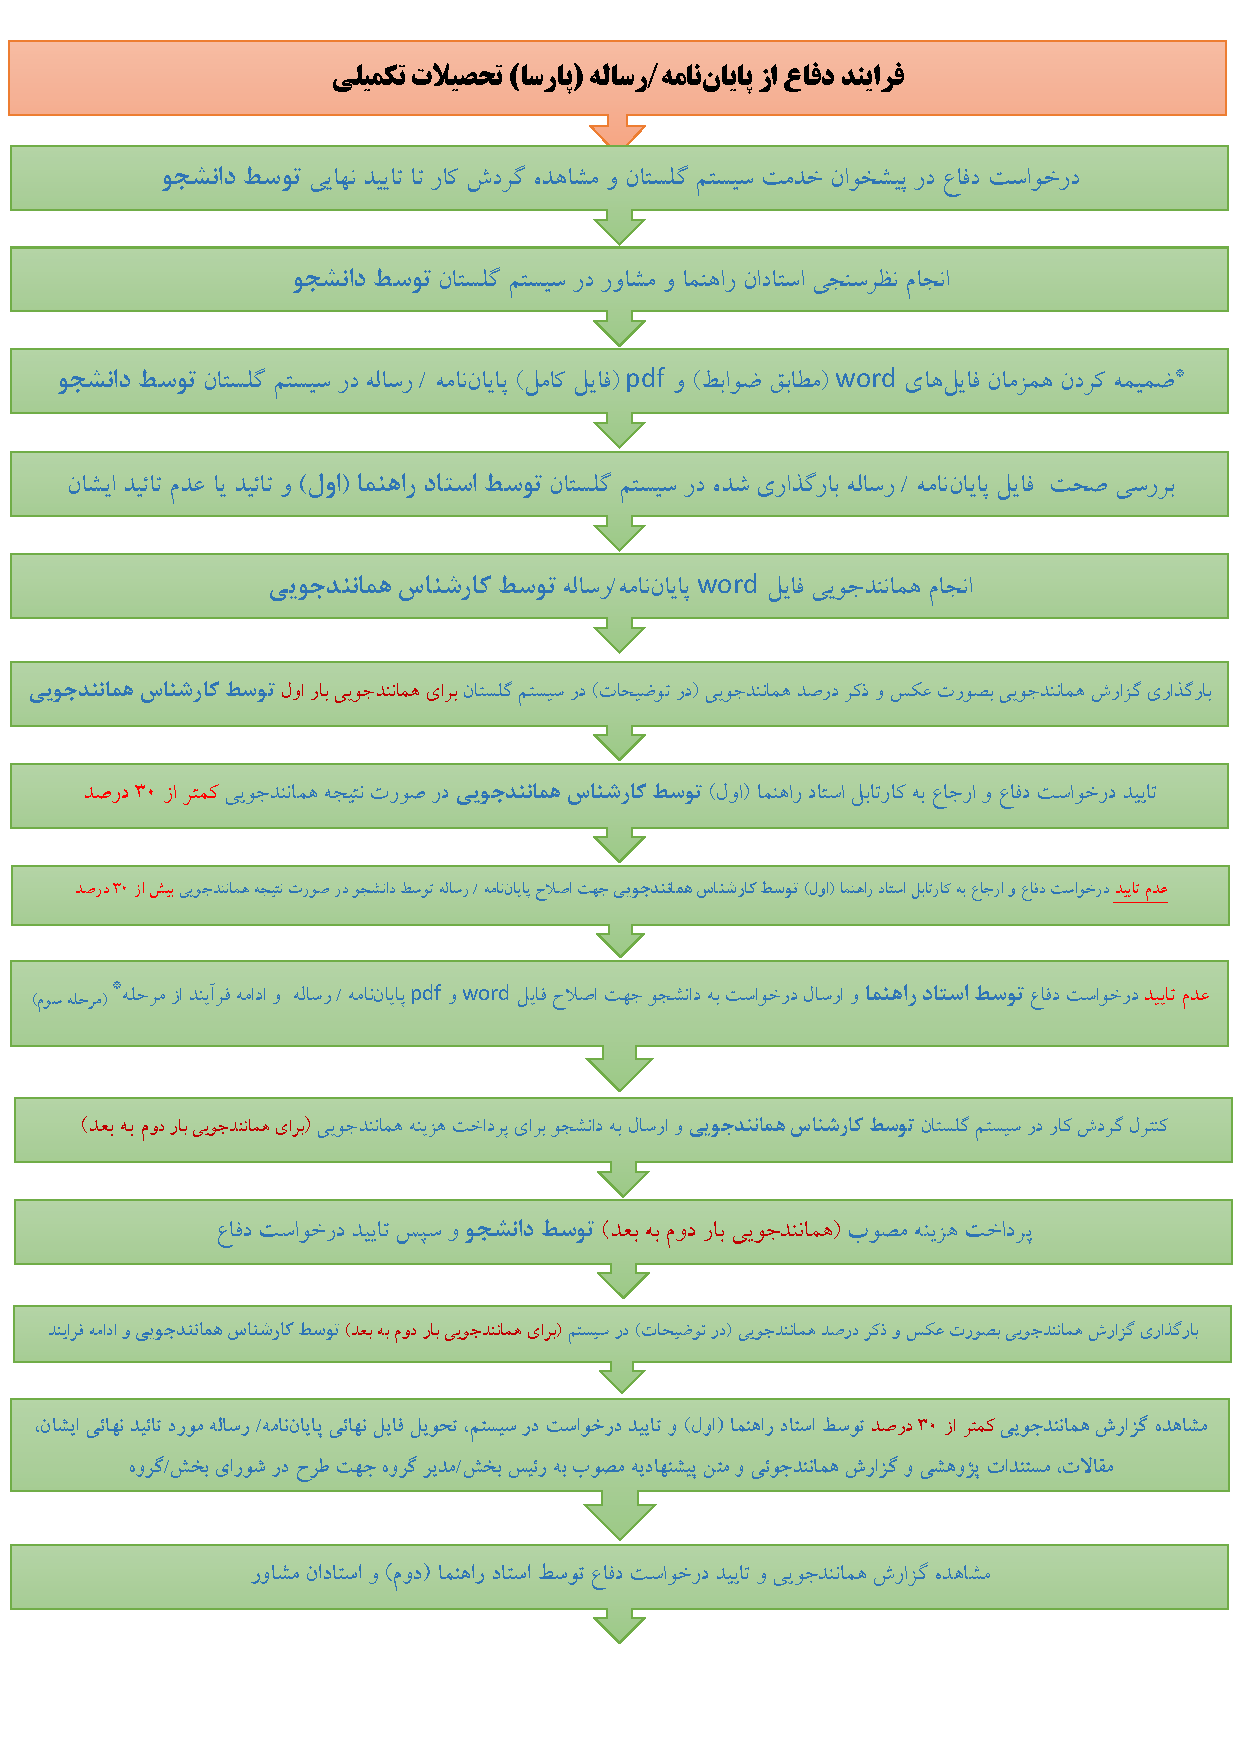
\includegraphics[width=0.95\textwidth]{defence-chart_Part1}}

\centerline{\includegraphics[width=\textwidth]{defence-chart_Part2}}

\section{توصیه‌های تحصیلات تکمیلی دانشگاه در خصوص پارساها}
این دستورالعمل به منظورآشنایی و آگاهی دانشجویان با نحوه نگارش و چگونگی تدوین و تنظیم مطالب یک تحقیق علمی (رساله) 
تهیه شده و ضروری است دانشجویان نکات مطرح شده در آن را هنگام تنظیم رساله رعایت نمایند.

\subsection{ بخش‌های رساله }

رساله باید مشتمل بر بخش‌های زیر باشد: 
\begin{enumerate}
\item شناسنامه یا صفحه عنوان (به زبان فارسی)
\item  شروع با ذکر نام خداوند
\item  صورت‌جلسه (فارسی) هیأت داوران جلسة دفاع از رساله 
\item  تعهدنامۀ رعایت حقوق معنوی دانشگاه یزد
\item  منشور اخلاق پژوهش
\item  تقدیم (اختیاری)
\item  سپاس و قدردانی (اختیاری)
\item  چکیده فارسی  
\item  فهرست مطالب
\item  فهرست شکل‌ها (در صورت داشتن شکل یا نمودار)
\item  فهرست جدول‌ها (در صورت داشتن جدول)
\item  فهرست نمادهای اختصاری و اختصارات (در صورت داشتن علائم، اختصارات و نمادهای اختصاری)
\item  پیشگفتار (اختیاری و با تصویب پردیس/دانشکده مستقل)
\item  متن اصلی که مشتمل بر فصل‌های مختلف از جمله مقدمه یا دیباچه، مروری بر منابع و مطالعات انجام شده و اهداف پژوهش، روش تحقیق، نتایج و تجزیه و تحلیل و تفسیر آنها، نتیجه‌گیری و پیشنهادها است. (مقدمه، فصل اول تلقی می‌شود.)
\item  واژه‌نامه فارسی به انگلیسی یا بالعکس (اختیاری و با تصویب پردیس/دانشکده مستقل و تایید شورای تحصیلات تکمیلی دانشگاه)
\item  فهرست منابع و مآخذ
\item  پیوست‌ها (در صورت وجود)
\item ABSTRACT (چکیده به زبان انگلیسی)
\item  شناسنامه یا صفحه عنوان (به زبان انگلیسی)
\end{enumerate}

\subsection{ حروف‌نگاری (تایپ) رساله}
\begin{enumerate}
 \item برای تایپ رساله از نرم‌افزار Word (نسخه 2013 یا بالاتر) یا LATEX استفاده شود و ترجیحاً متن اصلی با قلم 
BNazanin 14 (یا فونت مصوب پردیس/ دانشکده مستقل با تأیید شورای تحصیلات تکمیلی دانشگاه) باشد. 
متون انگلیسی با قلم \lr{Times New Roman 12} تایپ شود. برای تایپ رساله‌های رشتۀ ادبیات عرب ترجیحاً از قلم 
بدر عربی 15 استفاده شود.

\begin{center}
\begin{tabular}{|c|c|c|} \hline
نوع متن &	فونت فارسی	& فونت انگلیسی \\ \hline
متن عادی &	\lr{BNazanin 14}&	\lr{Times New Roman 12}\\ \hline
شماره صفحه‌ها	& \lr{BNazanin 12}	& \lr{Times New Roman 10}\\ \hline
عنوان فصل‌ها&	\lr{BNazanin Bold 18}	& \lr{Times New Roman Bold 16}\\ \hline
عنوان بخش‌ها	& \lr{BNazanin Bold 16}	& \lr{Times New Roman Bold 14}\\ \hline
عنوان زیربخش‌ها	& \lr{BNazanin Bold 14}	&\lr{Times New Roman Bold 12}\\ \hline
عنوان شکل‌ها/نمودارها و جدول‌ها	& \lr{BNazanin 12}	&\lr{Times New Roman 11}\\ \hline
سربرگ (Header) هر فصل &	\lr{BNazanin 12}	& \lr{Times New Roman 11}\\ \hline
\end{tabular}
\end{center}

\item  در صفحه‌های سمت چپ فایل رساله، فاصله شروع خط تا لبه راست صفحه 4 سانتیمتر -به غیر از سطر مطلع پاراگراف 
که تا لبه صفحه پنج سانتیمتر باشد. فاصله خط تا لبه بالای صفحه سه سانتیمتر، لبه پایین و لبه چپ صفحه 5/2 سانتیمتر باشد. 
در صفحه‌های سمت راست، فاصله شروع خط تا لبه راست صفحه 5/2 سانتیمتر ـ به‌غیر از سطر مطلع پاراگراف که تا لبه صفحه
 5/3 سانتیمتر باشد ـ فاصله خط تا لبه بالای صفحه سه سانتیمتر، لبه پایین صفحه 5/2 و لبه چپ 4 سانتیمتر باشد. 
 فاصله عنوان مطلب تا اولین سطر نوشـته شده 2 سانتیمتر و فاصله بین خطوط 1 سانتیمتر 
 (\lr{Line Spacing: Exactly 29 pt}) باشد. فاصله شماره صفحه از لبه پایین صفحه 1 سانتیمتر باشد. 
 این فواصل برای خطوط در تمام مراحل تدوین رساله اعم از شکل‌ها / نمودارها، جداول، فهرست، عکس‌ها و غیره باید رعایت شود.
\item  
 جدول‌هایی که در راستای طولی صفحه تنظیم می‌شوند، باید طوری قرار گیرند که متن بالای آنها در سمت عطف رساله واقع شود
 و همچنین شکل‌هایی که در راستای طولی صفحه تنظیم می‌شوند، باید طوری قرار گیرند که متن پایین آنها در سمت لبه 
 رساله قرار گیرد. شکل‌ها و جدول‌ها حتی‌المقدور داخل متن و در نزدیک‌ترین فاصله به محلی که ذکر شده، آورده شوند.

توجه: در تدوین و تایپ صفحه‌های رساله به غیر از صفحه‌های تقدیم و سپاسگزاری از هیچ‌گونه کادر تزئینی و تذهیب استفاده نگردد.
\item 
 سعی شود تا حد امکان از به کار بردن واژه‌های با الفبای انگلیسی در متن رساله فارسی خودداری شود و در صورت نیاز، 
معادل انگلیسی لغت‌ها، اصطلاح‌های فارسی یا افراد خاص به صورت پانویس در صفحه‌ مربوطه درج شود (فقط یک‌بار و 
در اولین بار استفاده از آن کلمه). 
پانویس‌ها زیر یک خط که به فاصله‌ 5/2 سانتیمتر از لبه چپ صفحه و حداقل 3 سانتیمتر از لبه پایینی و به طول مورد نیاز 
رسم می‌شود، نوشته شوند. (در هر صورت لازم است 5/2 سانتیمتر حاشیه پایین صفحه رعایت شود). پانویس‌ها در هر صفحه 
با گذاردن شماره 1، 2 و ... در گوشه‌ بالای انتهای کلمه در متن مشخص شوند. (در مورد اصطلاحات و عبارت‌های علمی، توصیه 
شود که تا حد امکان از معادل فارسی مناسب استفاده شود و در مورد اسامی افراد خارجی هم از روال یکسانی برای همه اسامی 
استفاده شود).
\item 
 در نگارش کلماتی نظیر آن‌ها و ... که از دو بخش تشکیل شده است ولی یک کلمه (یا مفهوم) محسوب می‌شود بایستی ارتباط 
بین دو بخش به‌صورت "جداکننده بدون فاصله" (فشردن کلیدهای Shift+Space بصورت همزمان در صفحه کلید استاندارد 
فارسی) رعایت شود.
\item 
 برای قرار دادن علائم نگارشی نظیر نقطه، ویرگول، علامت سوال، علامت تعجب و ... بایستی بین این علائم و کلمات قبل 
فاصله‌ای نباشد ولی بعد از آن یک فاصله ایجاد شود.
\item 
 در مورد پرانتز، بین عبارت‌های داخل پرانتز و پرانتز فاصله‌ای نباشد، اما بین پرانتزها و عبارت‌های دو طرف آن یک فاصله 
قرار گیرد.
\item 
 نوشتن کلماتی مانند به‌جز، به‌سرعت، به‌دقت و ... به‌صورت بجز، بسرعت، بدقت و ... اشتباه است و بایستی بصورت مجزا 
و با رعایت نیم‌فاصله نوشته شوند. برای اطلاع از جزئیات بیشتر می‌توان به منابعی نظیر "دستورخط فارسی"، "به‌نویسی" 
و... مراجعه کرد.
\item 
 علامت نقطه-ویرگول (؛) یا مکث میانه در مواردی استفاده می‌شود که مفهوم جمله ناتمام است.
\item 
 سعی شود از نوشتن پاراگراف‌های طولانی اجتناب شود. 
\item 
 توصیه می‌شود در انتهای هر فصل به‌جز فصل مقدمه، یک بخش جمع‌بندی یا خلاصه فصل وجود داشته باشد. (با تایید پردیس/ دانشکده مستقل).
\item 
 توصیه می‌گردد برای نوشتن فرمول‌ها و روابط ریاضی در نرم‌افزار Word، از افزونه یا نرم‌افزار Mathtype استفاده شود.
\item 
 فهرســت مطالب ارائه شده با توجه به قالب مورد تایید هر دانشکده/ گروه مستقل می‌تواند متفاوت از نمونه ذکر شده در این فایل باشد.
\item 
 توصیه می‌شود عنوان هر فصل بالای صفحات مربوط به آن فصل به‌صورت سربرگ (Header) آورده شود. 
\end{enumerate}
\subsection{ شماره‌گذاری}
\begin{enumerate}
\item  شماره‌گذاری صفحه‌ها

در هنگام شماره‌گذاری صفحه‌های رساله، موارد قبل از فهرست مطالب (موارد 1 الی 8 قسمت الف) هیچگونه شماره‌ای داده نشود. 
شماره‌گذاری فهرست‌ها و پیشگفتار با استفاده از حروف ابجد یا اعداد رومی انجام شود و شماره‌گذاری متن اصلی با استفاده از اعداد 
فارسی تا آخرین صفحه انجام شود. توجه گردد در صفحۀ اول هر فصل که عنوان فصل نوشته می‌شود، شماره‌ صفحه ذکر نشود، 
لیکن به حساب آید. شماره‌گذاری صفحه‌ها باید وسط و به فاصله 1 سانتیمتر از لبه پایین صفحه باشد.
\item 
 شماره‌ گذاری فصل‌ها، بخش‌ها و زیربخش‌ها

بخش‌ها و زیربخش‌های مختلف هر فصل با اعدادی نظیر 6-4 یا 6-4-2 مشخص می‌شود که عدد 6 شماره‌ فصل، عدد 4 شماره 
بخش و عدد 2 شماره قسمت است. شماره و عنوان هر فصل با قلم \lr{BNazanin 18 Bold} و عناوین بخش‌های مختلف 
هر فصل با قلم \lr{BNazanin 16 Bold} و عناوین قسمت‌های هر بخش با قلم \lr{BNazanin 14 Bold}
 تایپ شود (یا فونت‌های مصوب پردیس/ دانشکده مستقل و تأیید شورای تحصیلات تکمیلی دانشگاه). ضمناً عناوین فصل‌ها 
 و بخش‌های زیر فصل حتماً به صورت خودکار با استفاده از levelهای word تنظیم گردند.
\item 
 شماره‌ گذاری جدول‌ها، شکل‌ها 

برای شماره‌گذاری جدول‌ها و شکل‌ها در متن اصلی رساله از دو شماره که با خط فاصله از یکدیگر جدا می‌گردند، استفاده 
می‌شود به‌طوری‌که تمام جدول‌ها و شکل‌ها از ابتدا تا انتهای رساله به ترتیب دارای شماره 1، 2، ... و n برای هر فصل خواهند 
بود که شماره سمت چپ نشان‌دهنده ترتیب جدول / شکل و شماره سمت راست نشان‌دهنده شماره فصلی است که جدول / شکل 
در آن ذکر گردیده است. (مثلاً برای فصل 2: جدول 2-1، جدول 2-2 و ...، برای فصل 3: جدول 3-1، جدول 3-2 و ...). شماره‌گذاری 
جدول-ها، شکل‌ها و.... مستقل از همدیگر صورت می‌گیرد (البته قابل ذکر است که «نمودار»ها هم جزء «شکل»ها تلقی می شوند و نیاز
 به تیتر (عنوان) مجزایی ندارند). عنوان جدول‌ها در بالای آنها و عنوان شکل‌ها در زیر آنها ذکر می‌گردد.
شماره‌ای که در متن به شکل‌ها، جدول‌ها و ... اختصاص داده می‌شود، باید به همان صورت، در فهرست جدول‌ها، شکل‌ها و ... 
که قبل از شروع متن اصلی در رساله تنظیم می‌گردد، ذکر شود. فهرست مطالب، فهرست شکل‌ها و فهرست جدول‌ها و... به 
صورت خودکار در word ایجاد شود.
\item 
 شماره ‌گذاری روابط و فرمول‌ها

 فرمول‌ها در هر فصل به طور جداگانه و به ترتیبی که ظاهر می‌شوند (مانند جدول‌ها و شکل‌ها)، شماره‌گذاری گردد. 
 شماره‌گذاری روابط و فرمول‌های نوشته شده در متن اصلی رساله مشابه با جدول‌ها و شکل‌ها از ابتدا تا انتهای رساله به 
 ترتیب 1، 2، ... و n برای هر فصل و در پرانتز لحاظ خواهند شد. به‌طور مثال فرمول بیستم در فصل سوم به‌صورت (3-20) 
 نوشته می‌شود.
در مورد شماره‌گذاری قضیه‌ها، گزاره‌ها، لم‌ها، مثال‌ها و نظایر آنها در هر فصل به‌طور جداگانه و به-ترتیبی که در متن می‌آیند 
شماره‌گذاری می‌شوند؛ این شماره‌گذاری چنان است که شماره فصل در سمت راست و شماره قضیه (و نظایر آن) بعد از آن آورده
 شده و بین آنها از نقطه استفاده می‌شود. لازم است کلمه قضیه (و نظایر آن) و شماره آنها به صورت قلم سیاه (Bold) نوشته شده
 و پس از آن علامت دو نقطه (:) آورده شود. همچنین برای شروع اثبات کلمه اثبات همراه (:) به صورت قلم سیاه می‌آید؛ (معمولا 
 برای رشته‌های دانشکده علوم ریاضی و ...)
\end{enumerate}
\subsection{منابع و مآخذ}

لازم است در متن به کلیه منابعی که مورد استفاده قرار می‌گیرد، اشاره شود. مرجع دهی باید بر اساس قالب مورد تصویب 
دانشکده / گروه مستقل باشد و اگر دانشکده / گروه مستقل قالب خاصی را تعیین نکرده، از قالب APA استفاده شود.
در صورتی‌که از نرم‌افزار مدیریت مرجع استفاده نمی‌شود معمولا به یکی از دو روش زیر در متن به مراجع اشاره می‌گردد:

\begin{enumerate}
\item  مراجع به ترتیبی که در متن می‌آیند شماره‌گذاری شوند. در این روش، مراجع به ترتیب شماره در فهرست 
منابع و مآخذ ذکر گردد. 
\item 
مراجع به ترتیب حروف الفبایی نام خانوادگی نویسنده اول شماره‌گذاری گردیده، به همین ترتیب در فهرست منابع و مآخذ 
ذکر می‌شود.
القاب و عناوین دکتر، مهندس و … از جلوی نام مؤلف، مترجم حذف می‌گردد و همچنین اگر کتاب دارای دو نویسنده یا 
بیشتر باشد نام و نام خانوادگی همه آنها به ترتیبی که در روی جلد کتاب آمده است، آورده شود.

به‌طور مثال:

یاحقی، محمد جعفر و ناصح، محمد مهدی، راهنمای نگارش و ویرایش، چاپ هشتم، مشهد: آستان قدس رضوی، ص106.

در صورت وجود منابع به زبان‌های مختلف، توصیه‌ می‌شود مراجع غیرانگلیسی نیز به انگلیسی ترجمه و در 
انتها واژه‌ی (\lr{in Persian}) داخل پرانتز قید شده و سال آنها نیز به میلادی برگردان شوند. در غیر این صورت، 
ابتدا مراجع فارسی و سپس سایر مراجع ذکر شود. 
اگر شکل یا جدولی از منبع و مأخذی گرفته شده، لازم است مرجع آن در انتهای عنوان آن شکل یا جدول آورده شود.
\end{enumerate}
\subsection{شیوه‌نامه پردیس فنی و مهندسی}
برای دانشجویان پردیس فنی و مهندسی رعایت موارد ذیل الزامی است.
\begin{enumerate}
\item  استفاده از نرم‌افزار مدیریت مرجع مانندEndnote ، Mendeley و ... الزامی است.
\item  برای ارجاع بصورت شماره از قالب IEEE  و برای ارجاع با استفاد از نام و تاریخ از قالب APA استفاده شود.
\item  در صورت وجود منابع به زبان‌های مختلف، ضروری است مراجع غیرانگلیسی نیز به انگلیسی ترجمه و در انتها واژه‌ی
 (in Persian) داخل پرانتز قید شده و سال آنها نیز به میلادی برگردان شوند.
\end{enumerate}
\section{آماده‌سازی فایل جهت همانندجویی}
با توجه به نیاز به همانندجویی پیشنهادیه و پارساهای دانشگاه، لازم است کلیه دانشجویان در زمان درخواست دفاع با تصویب پیشنهادیه، 
فایل پیشنهادیه/پایان‌نامه با فرمت Word را در سامانه گلستان بارگذاری نمایند تا همانندجویی روی آن‌ها  انجام شود. 

برای دانشجویانی که از زیپرشن برای تایپ پایان‌نامه استفاده کرده‌اند، کافی است محتویات فایل \lr{.tex} را که محتوای پایان‌نامه آنها است را به 
همان صورت کپی و در یک فایل Word الصاق نمایند و فایل Word حاصل را برای همانندجویی بارگذاری دهند. لازم به ذکر است که نیاز به 
صفحات اولیه و مراجع پیشنهادیه/پایان‌نامه برای همانندجویی نیست.
 
راهکار دیگری که پیشنهاد می‌شود و البته مستلزم استفاده از ابزاری به نام GrindEQ است، این است که با نصب این ابزار، فایل اصلی پیشنهادیه/پایان‌نامه 
را در Word باز نمایید تا تمام پایان‌نامه به Word تبدل شود. البته این ابزار مجانی نیست، ولی برای هر نصب، تا 10 تبدیل را انجام می‌دهد. 
با این تبدیل، تمام فرمول‌ها و غیره کاملا منتقل می‌شود. تنها مشکل آن، نداشتن ساختار است و شکل‌ها نیز بعضا منتقل نمی‌شود که می‌شود دستی اصلاح 
کرد. البته برای همانندجویی، نیازی به داشتن شکلها نیست. راهنمای نصب و استفاده از این ابزار در بخش~\label{sec:grineq} آمده است.

%\newpage 
\subsection{ دستورالعمل ورود اطلاعات پایان‌نامه کارشناسی ارشد/ رساله دکتری توسط دانشجو در سامانه \lr{Irandoc}}
% پژوهشگاه علوم و اطلاعات ایران (Irandoc)}

\centerline{\includegraphics[width=0.6\textwidth]{Irandoc}}
\pagebreak 

\subsection{برخی نکات نگارشی}
در نوشتن مطالب علمی، رعایت قوانین نگارشی لازم است. در این کوتاه، صرفاً به برخی نکات نگارشی مهم اشاره می‌شود که لازم است در متن
پارساها به آن‌ها توجه شود. لازم به ذکر است که در خصوص برخی از قوانین نگارشی، ممکن است اختلاف نظری وجود داشته باشد ولی اکثر موارد 
ذکرشده مورد اتفاق است.
\begin{enumerate}
\item  علائم سجاوندی مانند کاما، ؛، .، :، ! و ؟ بدون فاصله با کلمه‌ی قبل از خود نوشته می‌شوند، ولی بعد از
آن‌ها باید یک فاصله‌ی خالی قرار گیرد. مانند: من، تو؛ او.
\item 
 علامت‌های پرانتز، آکولاد، کروشه، نقل‌قول و نظایر آن‌ها، بدون فاصله با عبارت داخل خود نوشته 
می‌شوند، ولی با عبارت اطراف خود یک فاصله دارند. مانند: (اين)،  (آن) و «آن‌ها».
\item 
  علامت استمرار «می» جدای از کلمه‌ی بعد خود و بی‌فاصله با آن (یعنی با نیم‌فاصله) نوشته می‌شود. مانند: می‌دهیم، می‌شود.
\item 
 علامت جمع «ها»، علامت صفت برتری «تر» و علامت صفت برترین «ترین»؛ جدای از کلمه‌ی قبل از خود و بی‌فاصله با آن  (یعنی با نیم‌فاصله) نوشته می‌شود. 
 مانند: آن‌ها بیش‌تر و کم‌ترین.
 
تبصره: کلمه‌های بهتر و بهترین از این قاعده مستثنا هستند.
\item 
 شناسه‌های «ام». «ایم»» «ای». «اید» و «اند» بی‌فاصله با کلمه‌ی قبل از خود  (یعنی با نیم‌فاصله) نوشته می‌شوند. ولی «است» با
فاصله است، مگر وقتی که کلمه‌ی قبلی با «ه» یا «ا» تمام شود. مانند: رفته‌ام رفته است. از ماست که برماست.
\item 
 ضمیرهای متصل جمع جدا ولی بدون فاصله با کلمه‌ی قبل خود  (یعنی با نیم‌فاصله) نوشته می‌شوند. مانند: زندگی‌مان؛
راه‌شان» ولی ضمیرهای متصل مفرد متصل نوشته می‌شوند. مانند: راهم نامت و کتابش.
\item 
 «به» هميشه جدا از کلمه‌ی قبل از خود ولی بدون فاصله  (یعنی با نیم‌فاصله) نوشته می‌شود. مگر در مواری که فعل ساخته
شود. مانند: به‌نام، به‌سزا، ببینیم.
\item 
 «به» هم‌واره جدا از کلمه‌ی قبل از خود ولی بدون فاصله نوشته می‌شود. مگر در مواری که حرف
اضافه‌ی «به» به تنهایی به‌کار رفته باشد. مانند: به‌سوی, به‌طرف، به آن‌ها.
\item 
‏ اجزای فعل با فاصله نوشته می‌شوند، مگر وقتی که یک جزء آن حرف اضافه باشد که در آن ‌صورت؛
حرف اضافه با کلمه‌ی بعد فاصله نخواهد داشت. مانند: تحریر کردن، درآورده شد، برآمده است، به‌کار
‏گرفتن.
\item 
 پیشوندها و پسوندهای جامد سرهم نوشته می‌شوند. مانند: دانشگاه، همسایه، همسر.
 
تبصره: در مورادی که خواندن کلمه دچار اشکال شود، می‌توان پسوند و پیشوند را جدا کرد. مانند: هم‌میهن، هم‌ارزی.
\item 
 اجزای حروف اضافه‌ی مرکب، قیدها، اسم‌ها، و صفت‌های مرکب بی‌فاصله نوشته می‌شوند. مانند: دراین‌صورت، آن‌گاه، به‌طوری‌که، کتاب‌خانه، دانش‌جو.
 \item 
 کلمه‌های مرکب دیگر نیز جدا و بدون فاصله نوشته می‌شوند. مانند: گفت‌وگو، پرس‌وجو و جست‌وجو.
 \item 
به‌دلیل دشواری خواندن، می‌توان «ها»ی ملفوظ را از قوانین جداسازی استثنا نمود. مانند: راهنما؛ رهبر.
\item 
 کسره‌ی اضافه‌ی بعد از «ه» به‌صورت «ه‌ی» نوشته می‌شود، نه «ۀ». مانند: خانه‌ی علی.
 
تبصره: اگر «ه» ملفوظ باشد. نباید «ی» را نوشت. مانند: فرمانده کل، پادشه خوبان.
\item 
 پایه‌های همزه در کلمه‌ها همیشه «ئ» است. مگر در مواری که همزه ساکن باشد. که دراین‌صورت باید
متناسب با اعراب حرف قبل نوشته شود. مانند: مسئله، مسئول، رأس، مؤمن.

تذکر: همزه‌ی بعد از حرف کشیده‌ی «ا» نوشته نمی‌شود. مانند: املا، استقرا، استثنا.
\item 
سعی شود جمع‌های کلمه‌های عربی به فارسی نوشته شود. مانند: شکل‌ها (به‌جای اشکال)، عبارت‌ها (به‌جای عبارات)، علامت‌ها (به‌جای علائم).
\item 
 جملات نقل‌قول یا موکد درون علامت نقل‌قول « و » قرار می‌گیرند. نه بین " *. مانند «استعداد خوب».
\item 
کلمه‌هایی که با جدانویسی خواناترند. جدا و بدون فاصله نوشته می‌شوند. مانند: چه‌گونه (به‌جای چگونه).
\item 
 «ی» عربی به‌صورت «» نوشته می‌شود. مگر آن‌که خوانند دچار مشکل شود. مانند: حتا و مستثنا.
 \item در کلمه‌های دو بخشی که به همراه هم یک مفهوم را مشخص می‌کنند، از نیم فاصله استفاده شود. مانند خوشه‌بندی، بهینه‌سازی، پیاده‌سازی و پایان‌نامه.
 یک راه  تشخیص، نگاه به کلمه انگلیسی معادل است. مثلاً \lr{clustering}  و \lr{optimization} و \linebreak 
 \lr{implementation} و \lr{thesis}.
 \item در استفاده از کاما برای روان‌تر شدن خواندن جملات استفاده شود. معمولاً هر جا در خواندن جمله یک توقف کوتاه رخ می‌دهد، باید کاما اضافه‌ شود.
 مانند «همچنان که در بخش قبل بیان شد، الگوریتم‌های ابتکاری کاربرد بسیاری در ....»
 \item حتی‌الامکان از معادل فارسی کلمات انگلیسی استفاده شود. مانند روش به جای تکنیک.
\end{enumerate}

\section{چند راهکار ساده اما راهگشا!}
یکی از وقت‌گیرترین کارهای آماده‌سازی یک متن علمی، مخصوصاً  در تجربه‌های اول، وفور خطاهای عمدتاً نگارشی است
که رفع آن‌ها، اولاً وقت زیادی می‌گیرد و ثانیاً نیاز به تمرکز بسیار دارد و حقیقتاً حوصله دانشجویان را به سر می‌برد. در این فصل راهکارهای ساده‌ای
ارائه می‌شود که می‌توانید این روند را سریع و بدون دردسر و با دقت زیاد انجام دهید.

\subsubsection{راهکار اول: از replace استقاده کنید!}
فرض کنید در پایان‌نامه، کلمه «می شود» را به همین صورت اشتباه استفاده کرده‌اید. لذا باید همه موارد استفاده شده به صورت «می شود» را به «می‌شود»
اصلاح نمایید. انجام این کار به صورت دستی و مورد به مورد بسیار مشکل است و در نهایت نیز مواردی از چشم شما پنهان می‌ماند. اما با استفاده از امکان
replace که تقریباً در تمام ادیتورها در دسترس هستند، می‌توانید این کار را در سرتاسر پایان‌نامه با صرف چند دقیقه و بدون نیاز به بررسی چشمی
انجام دهید. برای این کار replace ادیتور خود را انتخاب کنید (این کار در \lr{Notepad++} با کلید میانبر \lr{CTRL+H} می‌توانید انجام دهید).
سپس در قسمت \lr{Find}،  کلمه «می شود» و در قسمت \lr{Replace with}، کلمه «می‌شود» (هر دو بدون گیومه اول و آخر) قرار دهید. سپس گزینۀ
\lr{Find} را کلیک کنید و کلمه «می شود» بعدی را ببینید و اگر مایل به جایگزین هستید، گزینه \lr{Replace} را انخاب کنید. تکرار انتخاب ترتیبی
گزینه‌های \lr{Find} و \lr{Replace} به ترتیب اشکالات را پیدا و رفع می‌نماید. این کار را در تمام فایل‌های مربوط به پایان‌نامه خود تکرار کنید. اگر
از عدم وجود ترکیب‌های مشابه اطمینان دارید، می‌توانید با انتخاب گزینۀ \lr{Replace All}، همه اصلاحات را بدون چک کردن انجام دهید ولی برای 
استفاده از این گزینه دقت کنید زیرا ممکن است ترکیب مورد نظر شما در کلمات دیگری هم باشد که مایل به تغییر آن‌ها نباشید.

\subsubsection{راهکار دوم: استفاده از \lr{Inverse-Search}}
یکی از مشکلات کار با لاتک در مقایسه با \lr{Word} این است که متن نهایی با  متن نوشته شده متفاوت است. لذا اگر جایی از متن نیاز به
اصلاح داشته باشد، باید محل متناظر را در فایل tex یافت و سپس آن را اصلاح کرد. این کار، مخصوصاً اگر سند ما مفصل و چند ده صفحه‌ای باشد، بسیار
وقت‌گیر و خسته کننده است. اما اگر از \lr{SumatraPDF} استفاده کنید و نام پوشه و ابرپوشه‌های حاوی فایل سند شما فارسی نباشد، به راحتی با 
دوبار کلیک روی هر محل در فایل پی دی اف که در نرم‌افزار \lr{SumatraPDF} باز شده است، به محدوده همان محل در فایل tex مربوطه
منتقل می‌شوید. با این کار، عملاً نیاز به جستجوی طولانی مدت برای پیدا کردن محل ندارید.

\subsubsection{راهکار سوم: خطایابی و رفع خطا در بازه‌های زمانی کوتاه}
همانطور که در فیلم‌های آموزشی دوره مقدماتی لاتک آمده است، لاتک اصولاً یک زبان برنامه‌نویسی است که برای حروف‌چینی متون است. لذا، مشابه
یک برنامه، در صورت رعایت نشدن فرمت دستورات آن، در زمان حروف‌چینی با خطا مواجه خواهید شد. این خطا ممکن است به دلایلی نظیر
فراموش شدن یک علامت $\$$ یا  $\}$ باشد. البته، لاتک در صورت بروز خطا، تا بتواند کار را انجام می‌دهد اما اگر خطا به گونه‌ای باشد که کل کار را
مختل نماید، ممکن است بخشی یا کل متن حروف‌چینی نشود و در فایل پی دی اف نهایی نیاید. همانطور که در برنامه‌نویسی توصیه می‌شود، توصیه این است
که در زمان تایپ متن، در دوره‌های کوتاه‌مدت، متن را حروف‌چینی کنید و در صورت بروز خطا، آن را برطرف نمایید و پس از برطرف کردن کامل
خطاها، تایپ بخش بعدی را شروع نمایید. با این کار محدوده شما برای خطایابی کوچک بوده و معمولاً خطاها به سرعت پیدا و اصلاح می‌شوند.
\subsubsection{راهکار چهارم: گرفتن منظم نسخۀ پشتیبان}
هرچند فایل‌های لاتک، متنی هستند و مشابه فایل‌های ابزارهای مثل \lr{Word} نیستند که خراب شوند، ولی حذف شدن فایل یا رونویسی شدن
آن‌ها می‌تواند باعث از دست رفتن بخشی از کار شود. لذا توصیه کلی این است که نسبت به نسخه پشتیبان گرفتن از فایل‌های خود به طور منظم و در فواصل
نه چندان طولانی اقدام نمایید. همچنین می‌توانید ادیتور مورد استفاده خود را بررسی کنید و در صورت داشتن امکانات ایجاد فایل‌های پشتیبان به صورت
خودکار، آن را فعال نمایید.!
داخل فایل
\LRE{\verb!yazd-thesis-template.tex!}
و بعد از دستور
\verb!\chapter{راهنمای استفاده از کلاس \lr{yazd-thesis}}
\section{مقدمه}
حروف‌چینی پایان‌نامه یا رساله یکی از موارد پرکاربرد استفاده از زی‌پرشین است. از طرفی، یک  پایان‌نامه یا رساله،  احتیاج به تنظیمات زیادی از نظر صفحه‌آرایی  دارد که ممکن است برای
یک کاربر مبتدی، مشکل باشد. به همین خاطر، برای راحتی کار کاربر، کلاس حاضر با نام 
 \LRE{\verb!yazd-thesis!}
 برای حروف‌چینی پروژه‌ها، پایان‌نامه‌ها و رساله‌های دانشگاه یزد با استفاده از نرم‌افزار زی‌پرشین،  آماده شده است. این فایل به 
گونه‌ای طراحی شده است که کلیه خواسته‌های مورد نیاز  مدیریت تحصیلات تکمیلی دانشگاه یزد را برآورده می‌کند. همچنین حروف‌چینی بسیاری
از قسمت‌های آن، به طور خودکار انجام می‌شود.

کلیه فایل‌های لازم برای حروف‌چینی با کلاس گفته شده، داخل پوشه‌ای به نام
 \LRE{\verb!yazd-thesis!}
  قرار داده شده است. توجه داشته باشید که برای استفاده از این کلاس باید فونت‌های \lr{Yas}، \lr{Times New Roman}، 
  \lr{B Nazanin}  و \lr{Titr} روی کامپیوتر شما نصب باشد. این فونت‌ها در بین فونت‌های مشخص شده جهت نصب وجود دارد، ولی با توجه به این که
  ممکن است نصب \TeX{}Live از طریق دیگری انجام شده باشد، فونت‌های لازم در مسیر Fonts قرار گرفته است. می‌توانید این فونت‌ها را روی سیستم‌عامل
  خود نصب نمایید. تاکید می‌شود، در صورت نصب فونت، اگر با پیام وجود فونت روی کامپیوتر خود مواجه شدید، گزینه رونویسی فونت را انتخاب کنید تا از
  استفاده از نگارش مناسب فونت‌ها اطمینان حاصل نمایید.
 
\section{این همه فایل؟!}\label{sec2}
از آنجایی که یک پایان‌نامه یا رساله، یک نوشته بلند محسوب می‌شود، لذا اگر همه تنظیمات و مطالب پایان‌نامه را داخل یک فایل قرار بدهیم، باعث شلوغی
و سردرگمی می‌شود. به همین خاطر، قسمت‌های مختلف پایان‌نامه یا رساله  داخل فایل‌های جداگانه قرار گرفته است. مثلاً تنظیمات  کلاس داخل فایل
\LRE{\verb!yazd-thesis.cls!}، 
قسمت مشخصات فارسی پایان‌نامه داخل 
\LRE{\verb!fainfo.tex!}،
مطالب فصل اول، داخل 
\verb!chapter1!
و ... قرار داده شده است. نکته مهمی که در اینجا وجود دارد این است که از بین این  فایل‌ها، فقط فایل 
\LRE{\verb!yazd-thesis-template.tex!}
قابل اجرا است. یعنی بعد از تغییر فایل‌های دیگر، برای دیدن نتیجه تغییرات، باید این فایل را اجرا کرد. بقیه فایل‌ها به این فایل، کمک می‌کنند تا بتوانیم خروجی کار را ببینیم. اگر به فایل 
\LRE{\verb!yazd-thesis-template.tex!}
دقت کنید، متوجه می‌شوید که قسمت‌های مختلف پایان‌نامه، توسط دستورهایی مانند 
\verb!input!
و
\verb!include!
به فایل اصلی، یعنی 
\LRE{\verb!yazd-thesis-template.tex!}
معرفی شده‌اند. بنابراین، فایلی که همیشه با آن سروکار داریم، فایل 
\LRE{\verb!yazd-thesis-template.tex!}
است.
در این فایل، فرض شده است که پایان‌نامه یا رساله، از ۳ فصل و یک پیوست، تشکیل شده است. با این حال، اگر
  پایان‌نامه یا رساله، بیشتر از ۳ فصل و یک پیوست است، باید خودتان فصل‌های بیشتر را به این فایل، اضافه کنید. این کار، بسیار ساده است. فرض کنید بخواهید یک فصل دیگر هم به پایان‌نامه، اضافه کنید. برای این کار، کافی است یک فایل با نام 
\verb!chapter4!
و با پسوند 
\verb!.tex!
بسازید و آن را داخل پوشه 
\LRE{\verb!yazd-thesis!}
قرار دهید و سپس این فایل را با دستور 
\verb!\include{chapter4}!
داخل فایل
\LRE{\verb!yazd-thesis-template.tex!}
و بعد از دستور
\verb!\include{chapter3}!
 قرار دهید.
\section{از کجا شروع کنم؟}
قبل از هر چیز، بدیهی است که باید یک توزیع تِک مناسب مانند 
\verb!Live TeX!
و یک ویرایش‌گر تِک مانند
\verb!Texmaker!
یا
\verb!Notepad++!
را روی سیستم خود نصب کنید.  نسخه بهینه شده \verb!Texmaker!  را می‌توانید  از سایت 
 \href{http://www.parsilatex.com}{پارسی‌لاتک}%
\LTRfootnote{\url{http://www.parsilatex.com}}
 و \verb!Live TeX!  را هم می‌توانید از 
 \href{http://www.tug.org/texlive}{سایت رسمی آن}%
\LTRfootnote{\url{http://www.tug.org/texlive}}
 دانلود کنید.
 
در مرحله بعد، سعی کنید که  یک پشتیبان از پوشه 
\LRE{\verb!yazd-thesis!}
 بگیرید و آن را در یک جایی از هارددیسک سیستم خود ذخیره کنید تا در صورت خراب کردن فایل‌هایی که در حال حاضر، با آن‌ها کار می‌کنید، همه چیز را از 
 دست ندهید.
 
 حال اگر نوشتن پایان‌نامه یا رساله اولین تجربه شما از کار با لاتک است، توصیه می‌شود که یک‌بار به طور سرسری، کتاب «%
\href{http://mirror.ctan.org/tex-archive/info/lshort/persian/lshort.pdf}{مقدمه‌ای نه چندان کوتاه بر
\lr{\LaTeXe}}\LTRfootnote{\url{http://mirror.ctan.org/tex-archive/info/lshort/persian/lshort.pdf}}»
   ترجمه دکتر مهدی امیدعلی، عضو هیات علمی دانشگاه شاهد را مطالعه کنید. این کتاب، کتاب بسیار کاملی است که خیلی از نیازهای شما در ارتباط با حروف‌چینی را برطرف می‌کند.
 
 همچنین 10 جلسه فیلم آموزشی \LaTeX\  و  \XePersian\  نیز در لینک زیر در دسترس است که آموزش مقدماتی این دو است و با دیدن آن، 
 می‌توانید با موارد لازم آشنا شوید.
 \centerline{\url{https://farshi.blog.ir/1399/08/04/LaTeX-XePresian-Course}}
 
بعد از موارد گفته شده، فایل 
\LRE{\verb!yazd-thesis-template.tex!}
و
\LRE{\verb!fainfo!}
را باز کنید و مشخصات پایان‌نامه خود مثل نام، نام خانوادگی، عنوان پایان‌نامه و ... را جایگزین مشخصات موجود در فایل
\LRE{\verb!fainfo!}
 کنید. دقت داشته باشید که نیازی نیست 
نگران چینش این مشخصات در فایل پی‌دی‌اف خروجی باشید. فایل 
\LRE{\verb!yazd-thesis.cls!}
همه این کارها را به طور خودکار برای شما انجام می‌دهد. در ضمن، موقع تغییر دادن دستورهای داخل فایل
\LRE{\verb!fainfo!}
 کاملاً  دقت کنید. این دستورها، خیلی حساس هستند و ممکن است با یک تغییر کوچک، موقع اجرا، خطا بگیرید. برای دیدن خروجی کار، فایل 
\LRE{\verb!fainfo!}
 را 
\verb!Save!، 
(نه 
\verb!As Save!)
کنید و بعد به فایل 
\LRE{\verb!yazd-thesis-template.tex!}
برگشته و آن را اجرا کنید. حال اگر می‌خواهید مشخصات انگلیسی پایان‌نامه یا رساله را هم عوض کنید، فایل 
\LRE{\verb!eninfo!}
را باز کنید و مشخصات داخل آن را تغییر دهید.
در اینجا هم برای دیدن خروجی، باید این فایل را 
\verb!Save!
کرده و بعد به فایل 
\LRE{\verb!yazd-thesis-template.tex!}
برگشته و آن را اجرا کرد.

برای راحتی بیشتر، 
فایل 
\LRE{\verb!yazd-thesis.cls!}
طوری طراحی شده است که کافی است فقط  یک‌بار مشخصات پایان‌نامه یا رساله  را وارد کنید. هر جای دیگر که لازم به درج این مشخصات باشد، این مشخصات به طور خودکار درج می‌شود. با این حال، اگر مایل بودید، می‌توانید تنظیمات موجود را تغییر دهید. توجه داشته باشید که اگر کاربر مبتدی هستید و یا با ساختار فایل‌های  
\verb!cls!
 آشنایی ندارید، به هیچ وجه به این فایل، یعنی فایل 
\LRE{\verb!yazd-thesis.cls!}
دست نزنید.

نکته دیگری که باید به آن توجه کنید این است که چنانچه قصد حروف‌چینی رساله دکتری را دارید، 
 در فایل 
\LRE{\verb!yazd-thesis-template.tex!}
باید گزینه
\verb!msc!
را پاک کنید. با این کار، تنظیمات مربوطه به طور خودکار  اعمال می‌شود.    
\section{مطالب پایان‌نامه یا رساله را چطور بنویسم؟}
\subsection{نوشتن فصل‌ها}
همان‌طور که در بخش \ref{sec2} گفته شد، برای جلوگیری از شلوغی و سردرگمی کاربر در هنگام حروف‌چینی، قسمت‌های مختلف پایان‌نامه یا رساله از جمله فصل‌ها، در فایل‌های جداگانه‌ای قرار داده شده‌اند. 
بنابراین، اگر می‌خواهید مثلاً مطالب فصل ۱ را تایپ کنید، باید فایل‌های 
\LRE{\verb!yazd-thesis-template.tex!}
و
\verb!chapter1!
را باز کنید و محتویات داخل فایل 
\verb!chapter1!
را پاک کرده و مطالب خود را تایپ کنید. توجه کنید که همان‌طور که قبلاً هم گفته شد، تنها فایل قابل اجرا، فایل 
\LRE{\verb!yazd-thesis-template.tex!}
است. لذا برای دیدن حاصل (خروجی) فایل خود، باید فایل  
\verb!chapter1!
را 
\verb!Save!
کرده و سپس فایل 
\LRE{\verb!yazd-thesis-template.tex!}
را اجرا کنید. یک نکته بدیهی که در اینجا وجود دارد، این است که لازم نیست که فصل‌های پایان‌نامه یا رساله را به ترتیب تایپ کنید. می‌توانید ابتدا مطالب فصل ۳ را تایپ کنید و سپس مطالب فصل ۱ را تایپ کنید. 

نکته بسیار مهمی که در اینجا باید گفته شود این است که سیستم \lr{\TeX}، محتویات یک فایل تِک را به ترتیب پردازش می‌کند. به عنوان مثال، اگه فایلی، دارای ۴ خط دستور باشد، ابتدا خط ۱، بعد خط ۲، بعد خط ۳ و در آخر، خط ۴ پردازش می‌شود. بنابراین، اگر مثلاً مشغول تایپ مطالب فصل ۳ هستید، بهتر است
که دو دستور 
\verb!\include{chapter1}!
و
\verb!\include{chapter2}!
را در فایل 
\LRE{\verb!yazd-thesis-template.tex!}،
غیرفعال%
\RTLfootnote{
برای غیرفعال کردن یک دستور، کافی است پشت آن، یک علامت
\%
 بگذارید.
}
 کنید. زیرا در غیر این صورت، ابتدا مطالب فصل ۱ و ۲ پردازش شده (که به درد ما نمی‌خورد؛ چون ما می‌خواهیم خروجی فصل ۳ را ببینیم) 
 و سپس مطالب فصل ۳ پردازش می‌شود و این کار باعث طولانی شدن زمان اجرا می‌شود. زیرا هر چقدر حجم فایل اجرا شده، بیشتر باشد، 
 زمان بیشتری هم برای اجرای آن، صرف می‌شود.
 \subsection{محیط‌های شماره‌دار نظیر قضیه و لم}
 در قالب فعلی محیط‌های تعریف (\lr{definition})، مشاهده (\lr{observation})، قضیه (\lr{theorem})، لم (\lr{lemma})، 
 گزاره (\lr{proposition})، نتیجه (\lr{corollary})، ملاحظه (\lr{remark}) و مثال (\lr{example}) 
 تعریف شده‌اند. محیط‌های جدید نیز طبق آموزش‌های موجوددر ویدئوهای
 آموزشی دوره، قابل تعریف هستند.
 
در ادامه، به عنوان نمونه، چند تعریف، قضیه و مثال آورده شده است. 
\begin{definition}
مجموعه همه ارزیابی‌های  (پیوسته)  روی $(X,\tau)$، دامنه توانی احتمالی
\index{دامنه توانی احتمالی}
$ X $
نامیده می‌شود.
\end{definition}
\begin{theorem}[باناخ-آلااغلو]
\index{قضیه باناخ-آلااغلو}
اگر $ V $ یک همسایگی $ 0 $ در فضای برداری 
\index{فضای!برداری}
 توپولوژیکی $ X $ باشد و 
\begin{equation}\label{eq1}
K=\left\lbrace \Lambda \in X^{*}:|\Lambda x|\leqslant 1 ; \ \forall x\in V\right\rbrace,
\end{equation}
آنگاه $ K $،  ضعیف*-فشرده است که در آن، $ X^{*} $ دوگان
\index{فضای!دوگان}
 فضای برداری توپولوژیکی $ X $ است به ‌طوری که عناصر آن،  تابعی‌های 
خطی پیوسته
\index{تابعی خطی پیوسته}
 روی $X$ هستند.
\end{theorem}
تساوی \eqref{eq1} یکی از مهم‌ترین تساوی‌ها در آنالیز تابعی است که در ادامه، به وفور از آن استفاده می‌شود.
\begin{example}
برای هر فضای مرتب، گردایه 
$$U:=\left\lbrace U\in O: U=\uparrow U\right\rbrace $$
از مجموعه‌های بالایی باز، یک توپولوژی تعریف می‌کند که از توپولوژی اصلی، درشت‌تر  است.
\end{example}
حال تساوی 
\begin{equation}\label{eq2}
\sum_{n=1}^{+\infty} 3^{n}x+70x=\int_{1}^{n}8nx+\exp{(2nx)}
\end{equation}
را در نظر بگیرید. با مقایسه تساوی \eqref{eq2} با تساوی \eqref{eq1} می‌توان نتیجه گرفت که ...
 
 \subsection{الگوریتم‌ها}
 الگوریتم  \ref{alg:Fibonacci}  $n$امین عدد فیبوناچی را محاسبه می‌کند.

 \begin{algorithm}%[H]
%\SetLine 
\KwIn{ $n$.} \KwOut{$F(n)$.}
\eIf{$n==0$ \rl{یا} $1$ }{\Return n\;}{\Return Fib$(n-1)+$Fib$(n-2)$\;}
 \caption{Fib$(n)$}\label{alg:Fibonacci}
\end{algorithm}
برای بررسی زمان اجرای این الگوریتم، نگاهی به درخت اجرای آن برای محاسبه ششمین عدد فیبوناچی در شکل \ref{fig:Fibonacci}  می‌اندازیم:

\begin{figure*}[htb]
\begin{center}
\includegraphics[width=\textwidth]{Fibonacci} 
\end{center}
\caption{درخت اجرای الگوریتم \ref{alg:Fibonacci}
به ازای $n=6$.
}
\label{fig:Fibonacci}
\end{figure*}
تعداد برگ‌های درخت اجرای الگوریتم و در نتیجه زمان اجرای آن  نمایی است.


\subsubsection{مثال دوم}
مثالی دیگر برای محیط الگوریتم در الگوریتم~\ref{alg:Fastest-Way} آمده است.

 \begin{algorithm}%[H]
%\SetLine
 \KwIn{ $a, t, e, x, n$.} \KwOut{\rl{سریع‌ترین زمانِ تولید در کارخانه}}
$f_1[1]:=e_1+a_{1,1}$\;
$f_2[1]:=e_2+a_{2,1}$\;
\For{$j:=2$ to $n$}{
	\eIf{$f_1[j-1]+a_{1,j}\leq f_2[j-1]+t_{2,j-1}+a_{1,j}$}{
		$f_1[j]:=f_1[j-1]+a_{1,j}$\;
		$\ell_1[j]:=1$\;
	}{
		$f_1[j]:=f_2[j-1]+t_{2,j-1}+a_{1,j}$\;
		$\ell_1[j]:=2$\;
	}
	\eIf{$f_2[j-1]+a_{2,j}\leq f_1[j-1]+t_{1,j-1}+a_{2,j}$}{
		$f_2[j]:=f_2[j-1]+a_{2,j}$\;
		$\ell_2[j]:=2$\;
	}{
		$f_2[j]:=f_1[j-1]+t_{1,j-1}+a_{2,j}$\;
		$\ell_2[j]:=1$\;
	}
}
\eIf{$f_1[n]+x_1\leq f_2[n]+x_2$}{
	$f^*:=f_1[n]+x_1$\;
	$\ell^*:=1$\;
	}{
	$f^*:=f_2[n]+x_2$\;
	$\ell^*:=2$\;
	}
	\Return $f^*$\;
 \caption{{\sc FASTEST-WAY}$(a, t, e, x, n)$}\label{alg:Fastest-Way}
\end{algorithm}
  
 
 \subsection{مراجع}
مرجع \cite{Omidali82phdThesis} یک نمونه پروژه دکترا و مرجع \cite{Vahedi87} یک نمونه مقاله مجله فارسی است.
مرجع \cite{Amintoosi87afzayesh}  یک نمونه  مقاله کنفرانس فارسی و
مرجع \cite{vahid90} یک نمونه کتاب فارسی است. مرجع \cite{Khalighi07MscThesis} یک نمونه پروژه کارشناسی ارشد انگلیسی و
\cite{Khalighi87xepersian} هم یک نمونه متفرقه  می‌باشند.

مرجع \cite{Gonzalez02book} یک نمونه کتاب لاتین است که از آنجا که دارای فیلد \lr{authorfa} است، نام نویسندگان آن در استیلهای \lr{asa-fa}، \lr{plainnat-fa} و \lr{chicago-fa} به فارسی دیده می‌شود. مرجع \cite{Baker02limits} مقاله انگلیسی است که معادل فارسی نام نویسندگان آن ذکر نشده بوده است.

برای تولید مراجع باید از دستور \lr{bibtex} استفاده کنید. در صورتی که بخواهید مراجع فارسی قبل از
مراجع انگلیسی بیایند، باید به جای دستور \lr{bibtex thesis} از دستور زیر استفاده کنید:
\begin{latin}
\lr{bibtex8 -W -c cp1256fa thesis}
\end{latin}

توصیه دانشگاه، استفاده از قالب مراجع APA یا IEEE برای مراجع است که با استفاده از راهنمای bibtex، می‌توانید براحتی این کاررا انجام دهید.
البته با توجه به این که هنوز برای این قالب‌های مراجع، نسخۀ فارسی ارائه نشده است، در صورت داشتن مراجع فارسی، باید با شکل توصیه شده توسط 
دانشگاه، مراجع را به انگلیسی تبدیل کنید و در انتهای آن \lr{(in Persian)} اضافه نمایید.
دقت کنید که در صورت استفاده از قالب‌های مراجع انگلیسی (یعنی قالب‌هایی که با fa ختم نشده‌اند)، لازم است قبل از دستور مراجع، دستور 
\LRE{\verb!\latin!} 
و بعد از اتمام مراجع دستور 
\LRE{\verb!\persian!} 
را اضافه نمایید.
\subsection{واژه‌نامه فارسی به انگلیسی و برعکس}
برای وارد کردن واژه‌نامه فارسی به انگلیسی و برعکس، چنانچه کاربر مبتدی هستید، بهتر است مانند روش بکار رفته در فایل‌های 
\verb!dicfa2en!
و
\verb!dicen2fa!
عمل کنید. اما چنانچه کاربر پیشرفته هستید، بهتر است از بسته
\verb!glossaries!
استفاده کنید. راهنمای این بسته را می‌توانید به راحتی و با یک جستجوی ساده در اینترنت پیدا کنید.
\subsection{نمایه}
برای وارد کردن نمایه، باید از 
\verb!xindy!
استفاده کنید. زیرا 
\verb!MakeIndex!
با حروف «گ»، «چ»، «پ»، «ژ» و «ک» مشکل دارد و ترتیب الفبایی این حروف را رعایت نمی‌کند. همچنین، فاصله بین هر گروه از کلمات در 
\verb!MakeIndex!،
به درستی رعایت نمی‌شود که باعث زشت شدن حروف‌چینی این قسمت می‌شود. راهنمای چگونگی کار با 
\verb!xindy! 
را می‌توانید در تالار گفتگوی پارسی‌لاتک، پیدا کنید.

دستور مربوطه به صورت زیر است:

\begin{latin}
\footnotesize
\begin{verbatim}
xindy -L persian-variant2 -C utf8 -M texindy -M page-ranges yazd-thesis.idx
\end{verbatim}
\end{latin}

\subsection{تعریف نمادها و ایجاد فهرست نمادها}
ابتدا باید نمادها یکی یکی با استفاده از دستور
\LRE{\verb!\symbols{<symbol>}{<description>}!}
در متن  تعریف شوند. در این دستور منظور از 
\LRE{\verb!<symbol>!}
خود نماد است که در صورت ریاضی بودن آن، از 
\verb!$...$!
و در صورت ریاضی نبودن آن از دستور
\verb!\lr{...}!
برای نوشتن آن استفاده می‌شود. 
\LRE{\verb!<description>!}
هم توضیح و یا معنی نماد است. این دستور، نماد را در متن کتاب  چاپ می‌کند. دستور
\verb!\listofsymbol!
در فایل
\textsf{yazd-thesis.tex}
هم فهرست نمادها را چاپ می‌کند. 
%مقدار
%\verb![3em]!
%را می‌توانید در پایان کار، بسته به پهنای نمادها 
%کم و زیاد کنید. 


\section{چاپ فایل پی دی اف}
فایل پی دی اف حاصل از این بسته، مطمئناً مطابق با آیین‌نامه نگارش پایان‌نامه دانشگاه یزد
است و این امر توسط کارشناسان مرکز تحصیلات تکمیلی دانشگاه یزد تایید شده است.
اما چاپ فایل پی دی اف حاصل نیز باید به صورتی باشد که در خروجی تغییراتی داده نشود و نسخۀ
چاپ شده نیز مطابق با دستورالعمل باشد. 

 مشکل اصلی این است که برخی تنظیمات پرینتر، باعث ایجاد تغییرات در محصول نهایی می‌شود.
  حتی تغییر پرینتر نیز گاهی آنها را عوض می‌کند. 
 نکته‌ای که مشکل را حل می‌کند این است که، اولاً حتما مطمئن شوید 
 که اندازه کاغذ انتخابی در موقع پرینت، همان A4 باشد و ثانیاً تمام گزینه‌های مربوط 
 به \lr{Page Handling}  را غیرفعال کنید. نمونه به صورت شکل~\ref{print} است.
دقت کنید که بسته به پرینتر شما ممکن است موارد دیگری نظیر \lr{shrinking}  و غیره نیز 
موجود باشد که باید همه غیر فعال شوند.
با این ترتیب، مطمئنا حاشیه‌ها مطابق حاشیه‌ها در فایل پی دی اف خواهد بود.
\begin{figure}[!h]
 {\centerline{\includegraphics[width=0.7\textwidth]{Print-PDF}}}
 \caption{تنظیمات پرینتر در زمان چاپ.}\label{print}
 \end{figure}
\section{اگر سوالی داشتم، از کی بپرسم؟}
برای پرسیدن سوال‌های خود در مورد حروف‌چینی با زی‌پرشین،  می‌توانید به
 \href{http://qa.parsilatex.com}{سایت پرسش و پاسخ پارسی‌لاتک}%
\LTRfootnote{\url{http://qa.parsilatex.com}}
مراجعه کنید. شما هم می‌توانید روزی به سوال‌های دیگران در این سایت جواب بدهید. دقت کنید تا موارد ذکر شده در راهنماها  را به طور دقیق
و بدون کم یا زیاد انجام دهید. دلیل عمده اشکالاتی که رخ می‌دهد، عدم دقت در اجرای دقیق دستورالعمل‌ها است.
    
\subsection{سوالات پرتکرار}

{\bf سوال:} برخی کاراکتر‌ها در من من به صورت مربع نشان داده می‌شود. مشکل از کجاست؟
\\
{\bf جواب:} دلایل مختلفی برای ایجاد این مشکل وجود دارد. ابتدا، برای اطمینان از طی شدن همه مراحل نصب، مجدداً مراحل را چک کنید.
سپس، همین فایل پایان نامه را بدون ایجاد هر گونه تغییری اجرا نمایید. اگر اجرا بدون خطا پایان یافت و شما در این فایل با کاراکترهای جایگزین شده
با مربع روبرو شدید، دلیل آن عدم نصب شدن فونت‌های لازم روی کامپیوتر شماست. فونت‌های موجود در پوشه Fonts  را نصب کنید تا مشکل برطرف شود.
در صورت بروز خطا در اجرا، لازم است ابتدا اطمینان حاصل کنید که برای حروف‌چینی از دستور xelatex استفاده می‌شود. در صورتی که چنین است،
نصب شما مشکل دارد و باید مجدد با رعایت دقیق مراحل نصب ذکر شده در همین فصل، مجدداً نصب را انجام دهید.
در نهایت، حتما آموزش \LaTeX\ لازم است و بدون طی کردن دوره آموزشی آنلاین ذکر شده در این راهنما، با مشکلات متعدد روبرو خواهید شد که قادر به حل 
آن‌ها نمی‌باشید.
\\ \noindent
{\bf سوال:} متن فارسی به صورت کاراکترهای جدا از هم و حتی گاهی با ترتیب عکس نمایش داده‌ می‌شود. مشکل از کجاست؟
\\
{\bf جواب:} مهمترین دلیل این مشکل این است که متن فارسی را در محیط انگلیسی آورده‌اید. متن را دقیق چک کنید تا قبل از آن دستور 
\verb!\latin! نیامده باشد یا در داخل دستور \verb!\lr{...}!  یا محیط‌های مشابه نیامده باشد.
\\ \noindent
{\bf سوال:} آیا می‌توانم به جای \lr{\TeX{}Live} از \lr{Mik\TeX\ } استفاده کنم؟
\\
{\bf جواب:} از نظر اصولی بله ولی باید آخرین نگارش این نرم‌افزار را نصب نمایید. تجربه نشان داده است که \lr{\TeX{}Live} بهتر عمل می‌کند 
و با خطاهای کمتری کار را انجام می‌دهد. لذا توصیه به استفاده از آن می‌شود. دقت کنید که نگارش‌های قدیمی \lr{Mik\TeX\ } (مثل نگارش 9)
 به دلیل قدیمی بودن و نداشتن برخی ابزارها، قابلیت استفاده را ندارد.
!
 قرار دهید.
\section{از کجا شروع کنم؟}
قبل از هر چیز، بدیهی است که باید یک توزیع تِک مناسب مانند 
\verb!Live TeX!
و یک ویرایش‌گر تِک مانند
\verb!Texmaker!
یا
\verb!Notepad++!
را روی سیستم خود نصب کنید.  نسخه بهینه شده \verb!Texmaker!  را می‌توانید  از سایت 
 \href{http://www.parsilatex.com}{پارسی‌لاتک}%
\LTRfootnote{\url{http://www.parsilatex.com}}
 و \verb!Live TeX!  را هم می‌توانید از 
 \href{http://www.tug.org/texlive}{سایت رسمی آن}%
\LTRfootnote{\url{http://www.tug.org/texlive}}
 دانلود کنید.
 
در مرحله بعد، سعی کنید که  یک پشتیبان از پوشه 
\LRE{\verb!yazd-thesis!}
 بگیرید و آن را در یک جایی از هارددیسک سیستم خود ذخیره کنید تا در صورت خراب کردن فایل‌هایی که در حال حاضر، با آن‌ها کار می‌کنید، همه چیز را از 
 دست ندهید.
 
 حال اگر نوشتن پایان‌نامه یا رساله اولین تجربه شما از کار با لاتک است، توصیه می‌شود که یک‌بار به طور سرسری، کتاب «%
\href{http://mirror.ctan.org/tex-archive/info/lshort/persian/lshort.pdf}{مقدمه‌ای نه چندان کوتاه بر
\lr{\LaTeXe}}\LTRfootnote{\url{http://mirror.ctan.org/tex-archive/info/lshort/persian/lshort.pdf}}»
   ترجمه دکتر مهدی امیدعلی، عضو هیات علمی دانشگاه شاهد را مطالعه کنید. این کتاب، کتاب بسیار کاملی است که خیلی از نیازهای شما در ارتباط با حروف‌چینی را برطرف می‌کند.
 
 همچنین 10 جلسه فیلم آموزشی \LaTeX\  و  \XePersian\  نیز در لینک زیر در دسترس است که آموزش مقدماتی این دو است و با دیدن آن، 
 می‌توانید با موارد لازم آشنا شوید.
 \centerline{\url{https://farshi.blog.ir/1399/08/04/LaTeX-XePresian-Course}}
 
بعد از موارد گفته شده، فایل 
\LRE{\verb!yazd-thesis-template.tex!}
و
\LRE{\verb!fainfo!}
را باز کنید و مشخصات پایان‌نامه خود مثل نام، نام خانوادگی، عنوان پایان‌نامه و ... را جایگزین مشخصات موجود در فایل
\LRE{\verb!fainfo!}
 کنید. دقت داشته باشید که نیازی نیست 
نگران چینش این مشخصات در فایل پی‌دی‌اف خروجی باشید. فایل 
\LRE{\verb!yazd-thesis.cls!}
همه این کارها را به طور خودکار برای شما انجام می‌دهد. در ضمن، موقع تغییر دادن دستورهای داخل فایل
\LRE{\verb!fainfo!}
 کاملاً  دقت کنید. این دستورها، خیلی حساس هستند و ممکن است با یک تغییر کوچک، موقع اجرا، خطا بگیرید. برای دیدن خروجی کار، فایل 
\LRE{\verb!fainfo!}
 را 
\verb!Save!، 
(نه 
\verb!As Save!)
کنید و بعد به فایل 
\LRE{\verb!yazd-thesis-template.tex!}
برگشته و آن را اجرا کنید. حال اگر می‌خواهید مشخصات انگلیسی پایان‌نامه یا رساله را هم عوض کنید، فایل 
\LRE{\verb!eninfo!}
را باز کنید و مشخصات داخل آن را تغییر دهید.
در اینجا هم برای دیدن خروجی، باید این فایل را 
\verb!Save!
کرده و بعد به فایل 
\LRE{\verb!yazd-thesis-template.tex!}
برگشته و آن را اجرا کرد.

برای راحتی بیشتر، 
فایل 
\LRE{\verb!yazd-thesis.cls!}
طوری طراحی شده است که کافی است فقط  یک‌بار مشخصات پایان‌نامه یا رساله  را وارد کنید. هر جای دیگر که لازم به درج این مشخصات باشد، این مشخصات به طور خودکار درج می‌شود. با این حال، اگر مایل بودید، می‌توانید تنظیمات موجود را تغییر دهید. توجه داشته باشید که اگر کاربر مبتدی هستید و یا با ساختار فایل‌های  
\verb!cls!
 آشنایی ندارید، به هیچ وجه به این فایل، یعنی فایل 
\LRE{\verb!yazd-thesis.cls!}
دست نزنید.

نکته دیگری که باید به آن توجه کنید این است که چنانچه قصد حروف‌چینی رساله دکتری را دارید، 
 در فایل 
\LRE{\verb!yazd-thesis-template.tex!}
باید گزینه
\verb!msc!
را پاک کنید. با این کار، تنظیمات مربوطه به طور خودکار  اعمال می‌شود.    
\section{مطالب پایان‌نامه یا رساله را چطور بنویسم؟}
\subsection{نوشتن فصل‌ها}
همان‌طور که در بخش \ref{sec2} گفته شد، برای جلوگیری از شلوغی و سردرگمی کاربر در هنگام حروف‌چینی، قسمت‌های مختلف پایان‌نامه یا رساله از جمله فصل‌ها، در فایل‌های جداگانه‌ای قرار داده شده‌اند. 
بنابراین، اگر می‌خواهید مثلاً مطالب فصل ۱ را تایپ کنید، باید فایل‌های 
\LRE{\verb!yazd-thesis-template.tex!}
و
\verb!chapter1!
را باز کنید و محتویات داخل فایل 
\verb!chapter1!
را پاک کرده و مطالب خود را تایپ کنید. توجه کنید که همان‌طور که قبلاً هم گفته شد، تنها فایل قابل اجرا، فایل 
\LRE{\verb!yazd-thesis-template.tex!}
است. لذا برای دیدن حاصل (خروجی) فایل خود، باید فایل  
\verb!chapter1!
را 
\verb!Save!
کرده و سپس فایل 
\LRE{\verb!yazd-thesis-template.tex!}
را اجرا کنید. یک نکته بدیهی که در اینجا وجود دارد، این است که لازم نیست که فصل‌های پایان‌نامه یا رساله را به ترتیب تایپ کنید. می‌توانید ابتدا مطالب فصل ۳ را تایپ کنید و سپس مطالب فصل ۱ را تایپ کنید. 

نکته بسیار مهمی که در اینجا باید گفته شود این است که سیستم \lr{\TeX}، محتویات یک فایل تِک را به ترتیب پردازش می‌کند. به عنوان مثال، اگه فایلی، دارای ۴ خط دستور باشد، ابتدا خط ۱، بعد خط ۲، بعد خط ۳ و در آخر، خط ۴ پردازش می‌شود. بنابراین، اگر مثلاً مشغول تایپ مطالب فصل ۳ هستید، بهتر است
که دو دستور 
\verb!\include{chapter1}!
و
\verb!\chapter{راهنمای نصب  و استفاده از \LaTeX \ }
%شامل \XePersian}

\section{مقدمه}
نرم‌افزار حروف‌چینی \TeX یکی از نرم‌افزارهای معروف حروف‌چینی متون علمی است
که در سطح وسیعی جهت حروف‌چینی  مجلات و کتب استفاده می‌شود. در این متن مختصر بر آنیم
که راهنمای سریعی برای نصب و استفاده از آن بیان کنیم با این امید که کاربران با پیگیری آن
به راحتی  بتوانند آن را نصب و استفاده نمایند.

قبل از این لازم است جهت واضح شدن شکل عملکرد این نرم‌افزار، اطلاعاتی در مورد آن داشته
باشیم که در ادامه به آن پرداخته می‌شود.

نرم‌افزار حروف‌چینی \TeX\  یک نرم‌افزار مجانی است که به صورت خط فرمانی کار می‌کند، به این
معنی که متن مورد نظر در یک فایل نوشته شده و سپس این فایل از طریق دستورات خط
فرمان به نرم‌افزار حروفچین \TeX\  داده می‌شود. این نرم‌افزار فایل داده شده را خوانده و بر
مبنای آن متن حروف‌چینی شده را به صورت یک فایل (مثلا \lr{PDF}) ارائه می‌کند.

دستورات خط فرمان متعددی برای استفاده از این نرم‌افزار حروفچین وجود دارد که از مهمترین 
آنها می‌توان به \lr{latex}، \lr{pdflatex} و \lr{xelatex} اشاره کرد. معمولاً ما این بخش از
نرم‌افزار حروفچین را موتور \TeX\  می‌نامیم. این خاصیت، اولین متمایز کنندۀ این نرم‌افزار
از سایر نرم‌افزارها نظیر Office  است زیرا در Office شما نتیجه نهایی را همزمان با تایپ
 می‌بینید ولی در این نرم‌افزار باید فایل را به حروفچین بدهید تا خودش شکل خروجی را آماده
 کند. عملاً به همین دلیل نیز آن را نرم‌افزار حروفچین می‌نامند، مشابه این که شما متن خام 
 خود را به یک فرد حروفچین می‌دهید تا با شکل دهی آن در قالب صفحات، آن را برای چاپ
 آماده کند.
 
 پس متن خام باید در یک ویرایشگر تایپ شده و سپس فایل حاصل (که پسوند آن .tex است)
 به برنامۀ حروفچین
 با استفاده از خط فرمان داده شود. ویرایشگرهایی وجود دارند که امکان وارد کردن متن خام
 و به طور همزمان، امکان دادن فایل به موتور \TeX\  و نشان دادن نتیجۀ حروف‌چینی را دارند. 
 اما تمام آنها بر مبنای همان دستورات خط فرمان عمل می‌کنند و هیچکدام به تنهایی و بدون
 دسترسی به یک موتور \TeX\  نمی‌توانند خروجی تولید کنند. البته هیچ وابستگی بین
 ویرایشگر و فایل تولید شده توسط آن وجود ندارد و یک فایل توسط هر کدام می‌تواند 
 تولید یا ویرایش شود یا فایل ایجاد شده توسط  یک ویرایشگر، در دیگری تغییر یابد.
 از معروف‌ترین این ویرایشگرها می‌توان به \lr{\href{https://www.winedt.com/}{WinEdit}}، 
 \href{https://biditexmaker.software.informer.com/3.1/}{Texmaker}
و  \href{https://notepad-plus-plus.org/}{Notepad++}  اشاره کرد.

برای حروف‌چینی فایل، می‌توان از طریق خط فرمان به صورت زیر عمل کرد. در ویندوز
وارد \lr{Command Prompt } شوید و به محل قرار گرفتن فایل مربوطه (همان فایل با پیوند
.tex) بروید. بسته به کاربرد خود  و شکل خروجی مورد نظر 
یکی از دستورات زیر را بزنید تا فایل خروجی مربوطه ایجاد شود. به جای filename  نام
فایل .tex گذاشته شود. 


\begin{center}
\begin{tabular}{|c|c|}
\hline
برای خروجی .dvi با فایل ورودی انگلیسی & \lr{latex filename}\\  \hline
برای خروجی .pdf با فایل ورودی انگلیسی & \lr{pdflatex filename}\\ \hline
برای خروجی .pdf با فایل ورودی فارسی یا  انگلیسی & \lr{xelatex filename}\\ \hline
\end{tabular}
\end{center}

\textcolor{red}{\bf توجه مهم:} دقت کنید که نام فایل یا فولدرهایی که فایل در آن قرار دارد فارسی
نباشد یا بین نام آنها فاصله وجود نداشته باشد. در صورت عدم رعایت این موضوع، در برخی
مواقع اجرا با مشکل روبرو می‌شود.

فایل آماده شده خام، شامل دستوراتی است که قسمتهای مختلف متن نظیر عنوان فصل و بخش
و سایر موارد را مشخص می‌کند. اگر این دستورات درست استفاده نشده باشند، حروفچین در زمان
حروف‌چینی خطا می‌دهد که پیام خطا شامل شماره خطی است که در آن خطا اتفاق افتاده است.
لذا، در این موارد باید مشابه خطاگیری از یک برنامۀ کامپیوتری، نسبت به رفع خطا اقدام کرد.
توجه کنید که وجود خطا ممکن است متن را به صورتی به غیر از آنچه مورد نظر است حروف‌چینی
کند و اگر تعداد خطاها زیاد باشد ممکن است قسمت یا کل متن را حروف‌چینی نکند و خروجی
نداشته باشد یا خروجی حاصل ناقص باشد.
 
\section{نصب موتور اصلی \TeX\ }
توزیع‌های مختلفی برای موتور \TeX\  وجود دارد که در اینجا به نصب  توزیع
معروف و مجانی آن به نام‌ \lr{\TeX{}Live}  می‌پردازیم. تاکید می‌شود که  توزیع‌های مختلف با هم سازگار هستند، به این
معنی که فایل آماده شده روی تمام توزیع‌های موتور \TeX\  \ کار می‌کند. لذا مهم نیست کدام
توزیع را برای نصب انتخاب کنید. با نصب هر کدام از این دو توزیع، به طور اتوماتیک
بسته \XePersian \  نصب می‌شود و نیاز به هیچ کار اضافی نیست. 

البته توصیه پدیدآورندگان بسته \XePersian \ %که جهت تولید متون فارسی در \TeX\  \ 
%این بسته را ارائه کرده‌اند، 
استفاده از  \lr{\TeX{}Live}  است. 
%\pagebreak
\subsection{نصب \lr{\TeX{}Live 2020}}
%\footnote{با توجه به ارائه نسخه 2015 از TeXLive، این
%نسخه از طریق وبسایت اعلام شده در این قسمت وجود دارد. اما فعلاً این نگارش مشکلاتی با \XePersian دارد. و لذا  نسخه 2014 این نرم‌افزار را که در اف تی پی دانشگاه یزد وجود دارد دانلود و نصب نمایید. 
%مشکل
%را در \href{http://qa.parsilatex.com/7838/%D9%85%D8%B4%DA%A9%D9%84%D8%A7%D8%AA-texlive-2015-%D9%88-%D8%A7%D8%B1%D8%AA%D9%82%D8%A7-%D8%A8%D8%B3%D8%AA%D9%87-%D9%87%D8%A7-%D8%AF%D8%B1-texlive-2014?show=7838#q7838}{این لینک} ببینید.
%}
سایت‌های معروف به \lr{CTAN}، سایت‌هایی هستند که  وظیفه توزیع نسخه‌های مختلف
مجانی موتور \TeX\  را انجام می‌دهند. یکی از این وبسایت‌ها در  دانشگاه یزد 
قرار دارد که در آدرس 
\href{http://ctan.yazd.ac.ir/}{http://ctan.yazd.ac.ir/}
در دسترس است.\footnote{این وبسایت به همت آقای
مهندس فاطمی از مرکز اطلاع‌رسانی و خدمات رایانه‌ای دانشگاه یزد ایجاد شده است.
% که جا دارد از ایشان در این خصوص تشکر کرد.
}



این سایت به صورت روزانه به‌روزرسانی می‌شود. می‌توان از این سایت در هر 
لحظه آخرین نگارش‌های نرم‌افزارهای مربوطه را دانلود کرد. لازم به ذکر است که در صورت اتصال
به شبکه دانشگاه یزد، برای دسترسی به این سایت نیازی به استفاده از اکانتینگ و 
اتصال به اینترنت نیست، بلکه این سایت از طریق شبکه داخلی دانشگاه در دسترس است.\footnote{فایل‌های مورد استفاده علاوه بر آدرس‌های ذکر شده، در اف تی پی دانشگاه یزد 
به آدرس \url{http://ftp.yazd.ac.ir/} و ذیل پوشه "نرم افزارهای کاربردی ویندوز->\lr{ TeX}" قرار گرفته است.
کاربران متصل به شبکه دانشگاه یزد می‌توانند بدون  نیاز به اتصال به اکانتینگ، 
این فایل‌ها را با سرعت بالا دانلود نمایند.  دوستان می‌توانند از لینک گوگل درایو زیر نیز
 برای دانلود استفاده نمایند. 
حجم فایل حدود 4 گیگابایت است.
\url{https://drive.google.com/file/d/11dnlN7r3s3lXWWwV3JQ-a8JUjj3H2yZs/view?usp=sharing}
}


برای نصب \lr{\TeX{}Live}  مراحل زیر را انجام دهید:
\begin{enumerate}
\item وارد سایت \href{http://ctan.yazd.ac.ir/}{http://ctan.yazd.ac.ir/}
 شوید و در پایین صفحه روی \lr{TeX Live}
 کلیک کنید.
 \item روی مسیر Images کلیک کنید و از فولدر باز شده فایل با نام 
 	\lr{texlive2020-20200406.iso} را دانلود کنید. دقت کنید که 8 شماره آخر فایل ممکن 
	است مختلف باشد زیرا نشان‌دهنده تاریخ ایجاد فایل است. دقت کنید که حجم این فایل
	حدود \lr{3.7} گیگا بایت است.
 \item پس از دانلود کامل، آن را با نرم‌افزار WinRaR  باز کنید و در  پوشه‌ای به نام
 \lr{TeXLive2020} فایل را Extract کنید.
 \item وارد این پوشه شوید و برنامه 
 %install-tl
\lr{install-tl-windows}
 را اجرا کنید. ادامه روند مشابه نصب سایر نرم‌افزارها 
 است. روند نصب بسته به سرعت کامپیوتر شما ممکن است تا بیش از 2 ساعت طول بکشد. توصیه می‌شود جهت افزایش سرعت نصب و جلوگیری از تداخل ممکن، آنتی ویروس خود را قبل از شروع نصب، غیرفعال کنید.
 تصویر پنجره‌های نصب به صورت زیر است (به ترتیب از چپ به راست و از بالا به پایین). دقت کنید که باید تا ظاهر شدن آخرین پنجره که حاوی پیام
 \lr{Welcome to TeXLive!} است و فعال شدن دکمه \lr{Close} منتظر بمانید. در صورت بستن پنجره قبل از این، نصب کامل نشده است و امکان استفاده وجود ندارد.
\latin
\begin{figure}[htb]
\includegraphics[width=0.35\textwidth]{TexLive2020-installer}\hfill
\includegraphics[width=0.5\textwidth]{TexLive2020-installer-2}
\vspace*{4mm}

\includegraphics[width=0.45\textwidth]{TexLive2020-installer-3}\hfill
\includegraphics[width=0.50\textwidth]{TexLive2020-installer-4}
%\vspace*{4mm}

%\includegraphics[width=0.45\TeX\ \ twidth]{TexLive2015-5}\hfill
%\includegraphics[width=0.45\textwidth]{TexLive2015-6}
%\vspace*{4mm}
%
%\includegraphics[width=0.45\textwidth]{install-6}
\persian
\caption{پنجره‌های نصب \lr{\TeX{}Live2020} (ترتیب از چپ به راست)}
\end{figure}

\persian

 \item پس از پایان نصب، موتور \TeX\  آماده استفاده است. اگر قصد استفاده از \XePersian
 \ دارید، فقط لازم است فونت‌های مربوطه را که در بالا لینک آن آمده است را نصب کنید. عملاً نصب \lr{\TeX{}Live2020} در این مرحله پایان یافته است که شامل \XePersian \ نیز هست.
\end{enumerate}

\subsection{نصب فونت‌های  فارسی}
لازم است
که فونت‌های فارسی استفاده شده در متون فارسی روی سیستم عامل نصب شده باشد. لذا
تنها کار اضافی این است که مجموعه فونت‌های جمع آوری شده در فایل زیر روی سیستم عامل
نصب شود. توصیه می‌شود حتی اگر فونت‌ها را روی کامپیوتر خود دارید، دوباره آنها را با استفاده
از فونت‌های فایل زیر رونویسی کنید. این کار از بسیاری مشکلات بعدی جلوگیری می‌کند.
\begin{latin}

\href{http://bayanbox.ir/id/4609192605141061595}{Part 1: http://bayanbox.ir/id/4609192605141061595}

\href{http://bayanbox.ir/id/5468937351173971771}{Part 2: http://bayanbox.ir/id/5468937351173971771}

\href{http://bayanbox.ir/id/4133277893427051503}{Part 3: http://bayanbox.ir/id/4133277893427051503}
\end{latin}


\persian
\section{سایر ابزارهای مفید}
\subsection{ادیتور  Notepad++}
نرم‌افزار حروف‌چین \TeX\   دارای GUI مخصوص به خود نیست و روش کار با آن به این صورت است که فایل مربوط به متن مورد نظر ابتدا با استفاده از یک ادیتور، آماده‌سازی می‌شود و سپس، فایل با استفاده از دستورات خط فرمان، به موتور \TeX\  جهت حروف‌چینی داده می‌شود و حاصل این حروف‌چینی به صورت یک فایل پی دی اف تحویل می‌گردد. ادیتورهای متعددی برای این منظور وجود دارد و قابل استفاده است. از بین آنها، به نصب ادیتور \lr{Notepad++} می‌پردازیم.

ادیتور \lr{Notepad++ }  به دلیل قابلیت فارسی‌نویسی و همچنین از راست به چپ نویسی و امکان اجرای دستورات خط فرمان در ادیتور،
انتخاب مناسبی برای نوشتن متون  است. این نرم افزار متن باز از طریق وبسایت \href{https://notepad-plus-plus.org/}{https://notepad-plus-plus.org/} قابل دریافت است.

نصب نرم‌افزار، مشابه سایر نرم‌افزارها است و پیچیدگی خاصی ندارد. پس از نصب، برای فعال کردن قابلیت اجرای دستورات خط فرمان با استفاده از کلید \lr{F6}، باید افزونه \lr{NppExec} روی این نرم‌افزار نصب شود.

برای نصب این افزونه، پس از ورود به نرم‌افزار \lr{Notepad++}، وارد  منوی \lr{Plugins} و سپس \lr{Plugins Admin} شوید تا پنجره مطابق شکل زیر باز شود. در پنجره باز شده ابتدا در قسمت \lr{Search}، کلمه \lr{Nppexec} را وارد کنید، سپس مربع کنار این افزونه را تیک بزنید\footnote{در شکل، این افزونه به دلیل نصب بودن روی \lr{Notepad++} وجود ندارد ولی در لیست شما باید باشد.} و سپس روی \lr{Install} کلیک کنید.
\latin
\begin{figure}[htb]
\includegraphics[width=0.4\textwidth]{Notepad-1}\hfill
\includegraphics[width=0.55\textwidth]{Notepad-2}
%\vspace*{4mm}
%
%\includegraphics[width=0.45\textwidth]{TexLive2020-installer-3}\hfill
%\includegraphics[width=0.50\textwidth]{TexLive2020-installer-4}
\persian
\caption{پنجره‌های نصب \lr{NppExec} (ترتیب از چپ به راست)}
\end{figure}

\persian
 حال با زدن کلید \lr{F6}  در ادیتور، پنجره اجرای دستور به صورت شکل~\ref{NPPEXEC} باز می‌شود.
 \latin
\begin{figure}[htb]
\centerline{
\includegraphics[width=0.45\textwidth]{NppExec-1}\hfill
\includegraphics[width=0.45\textwidth]{NppExec-2}
}
\persian
\caption{پنجره‌ ورود دستورات در \lr{NppExec} (ترتیب از چپ به راست)}\label{NPPEXEC}
\end{figure}
\persian 

نمونه دستوری که می‌توانید وارد کنید به صورت زیر است:

\begin{latin}
\begin{verbatim}
NPP_SAVE
cd $(CURRENT_DIRECTORY)
xelatex $(NAME_PART)
\end{verbatim}
\end{latin}
 
 می‌توان دسته دستورات مختلفی را داشت و با کلیک روی \lr{Save}، با نام‌های مختلف آن را ذخیره کرد و برای استفاده‌های بعدی داشت. 
 
 چند نکته که مفید فایده است، به شرح زیر است.
 
برای تایپ از راست به چپ کلیدهای Alt+CTRL+R  را بزنید و برای از چپ به راست نویسی کلیدهای Alt+Ctrl+L  را بزنید.

برای نیم فاصله، کلید استاندارد \lr{Ctrl+SHift+2}  است که در این ادیتور به دلیل استفاده از این ترکیب برای کار دیگری عمل نمی‌کند.
برای عمل کردن آن باید این ترکیب کلید را از ادیتور حذف کنید. برای این منظور از منوی \lr{settings -> Shortcut Mapper}
 در برگه \lr{Main Menu}  در ردیف حدودا 80  این ترکیب را پیدا کرده و به چیز دیگری (مثلا \lr{CTRL+Shift+T}) عوض کنید.
 پس از این کار، ترکیب  \lr{Ctrl+SHift+2} برای نیم فاصله (وقتی زبان صفحه کلید فارسی باشد) کار می‌کند.
 
 توجه: برای تهیه فایل مقاله یا کتاب با \XePersian، باید از کد رمزگذاری \lr{UTF8}  برای کدگذاری فایل استفاده شود. برای انتخاب در ادیتور، از منوی
 Encoding  گزینه مورد نظر انتخاب شود.
 \subsection{نرم‌افزار \lr{Sumatra PDF}}
 نرم‌افزارهای متعددی برای مشاهده فایل‌های پی دی اف وجود دارد که مشهورترین آنها \lr{Adobe Acrobat} است. در استفاده از لاتک، فایل پی دی اف مکرر تغییر می‌کند و مجدد توسط نرم‌افزار حروف‌چین بازنویسی می‌شود ولی به دلیل قفل شدن فایل پی دی اف توسط بسیاری از نرم‌افزارهای مشاهده فایل پی دی اف؛ در روند حروف‌چینی خلل ایجاد می‌شود. لذا، توصیه می‌شود از نرم‌افزار \lr{Sumatra PDF} برای مشاهده فایل‌های پی دی اف در کنار تک استفاده شود. این نرم‌افزار، متن باز است و از طریق وبسایت \href{https://www.sumatrapdfreader.org/}{https://www.sumatrapdfreader.org/} قابل دریافت است.
 %
 \subsection{قالب پیشنهادیۀ  دانشگاه یزد}
 در جهت سهولت آماده‌سازی پیشنهادیۀ کارشناسی ارشد و دکتری  دانشگاه یزد، قالب مربوطه برای زیپرشن آماده‌سازی شده است و از طریق  
 %\href{http://farshi.blog.ir/1399/09/22/\%D9\%82\%D8\%A7\%D9\%84\%D8\%A8-\%D9\%BE\%D8\%B1\%D9\%88\%D9\%BE\%D9\%88\%D8\%B2\%D8\%A7\%D9\%84-\%DA\%A9\%D8\%A7\%D8\%B1\%D8\%B4\%D9\%86\%D8\%A7\%D8\%B3\%DB\%8C-\%D8\%A7\%D8\%B1\%D8\%B4\%D8\%AF-\%D8\%AF\%D8\%A7\%D9\%86\%D8\%B4\%DA\%AF\%D8\%A7\%D9\%87-\%DB\%8C\%D8\%B2\%D8\%AF-\%D8\%AF\%D8\%B1-\%D8\%B2\%DB\%8C\%D9\%BE\%D8\%B1\%D8\%B4\%D9\%86}{این لینک }
 \href{https://yazd.ac.ir/4063-70-5324}{لینک پیشنهادیه کارشناسی ارشد}
 و
 \href{https://yazd.ac.ir/4063-70-5442}{لینک پیشنهادیه دکتری}
 در دسترس است. فیلم راهنمای استفاده نیز در دوره آموزش مقدماتی لاتک در در بخش پایانی این فصل آمده است.
 لازم به ذکر است که با توجه به تغییرات در قالب پیشنهادیۀ دانشگاه، ممکن است برخی تفاوت‌ها در فیلم و قالب فعلی باشد.
 %
 \subsection{کلاس پایان‌نامه دانشگاه یزد}
 با توجه به تنظیمات خاص پایان‌نامه‌های دانشگاه‌های مختلف و وقت قابل ملاحظه‌ای که انجام این تنظیمات از دانشجویان می‌گیرد، 
 کلاسی بر مبنای تنظیمات پایان‌نامه‌های دانشگاه یزد ایجاد شده است. این قالب از مردادماه 1398 در \lr{CTAN} قرار 
 گرفته است و به همراه نصبٍ \lr{\TeX{}Live}
 نصب می‌شود و نیاز به هیچ کاری جهت نصب نیست. 
 نمونه فایل پایان‌نامه از طریق وبسایت زیر در دسترس دانشجویان عزیز می‌باشد.
 
 \centerline{\href{http://yazd-thesis.blog.ir/}{http://yazd-thesis.blog.ir/}}
 
 در این کلاس کلیه تنظیمات مربوط به پایان‌نامه لحاظ شده و نیاز به انجام تنظیمات اضافی ندارد. 
 توضیحات استفاده از این کلاس و فایل نمونه در وبسایت فوق آمده است.
 
 لینک فیلم راهنمای استفاده نیز در دوره آموزش مقدماتی لاتک در در بخش پایانی این فصل آمده است.
 %\pagebreak
 \subsection{تبدیل فایل‌های Word  به \LaTeX\   و برعکس} \label{sec:grineq}
 یک نرم‌افزار قوی برای تبدیل بین Word  و \LaTeX، نرم‌افزار \href{http://www.grindeq.com/}{GrindEQ}  است.\footnote{این راهنما بر مبنای ورژن این نرم‌افزار در سال 1395 تهیه شده است. استفاده ورژن‌های جدید ممکن است کمی متفاوت باشد.}
 این نرم‌افزار مجانی نیست ولی تا 10 فایل را برای شما تبدیل می‌کند. برای انجام تبدیل لازم است نرم‌افزار \lr{Office}  را نصب و سپس
 دو فایل مربوط به تبدیل بین Word  و \LaTeX  (در پوشه Convert وجود دارد) را نصب نمایید.
 برای نسخه‌های بعدی \lr{Office}، آخرین نگارش نرم‌افزار را از وبسایت فوق دریافت و نصب نمایید. نرم‌افزار منطبق بر آفیس را (از حیث 32 بیتی یا 64 بیتی بودن) را نصب کنید وگرنه عملکرد تبدیل مناسب نخواهد بود.
 \subsubsection{تبدیل Word به \LaTeX}
 فایل خود را در Word باز کنید. سپس از منوی \lr{File}،
 \lr{Save As}  را انتخاب کنید و در قسمت \lr{Save as Type}، نوع \lr{LaTeX[GrindEQ]}
 را انتخاب کنید.  از پنجره باز شده گزینه‌های مناسب را انتخاب و فایل را ذخیره کنید. فایل ذخیره شده با فرمت \LaTeX \  است.
 
 اگر فایل Word شما \textcolor{red}{\bf فارسی} است، باید از پنجره باز شده، در قسمت encoding، 
 گزینۀ \lr{UTF8} یا \lr{Unicode}  را انتخاب کنید. (شکل~\ref{Grindeq} را ببینید.) در فایل
 \LaTeX \ ایجاد شده نیز باید دستور \verb+ \usepackage{xepersian}+  و دستورات مربوط به فونت متن اضافه شود.
 
 همچنین در قسمتهای انگلیسی باید دستور \verb+\latin+  قبل از متن انگلیسی و \verb+\persian+ بعد از متن انگلیسی قرار گیرد.
 
 \subsubsection{تبدیل \LaTeX \ به Word}
  در Word   فایل \LaTeX  را باز کنید (فایل با پسوند \lr{.tex}). از پنجره باز شده مشابه قبلی، گزینه‌های مناسب را انتخاب کنید. فایل  به فرمت 
  Word تبدیل شده و باز می‌شود و می‌توانید آن را ذخیره کنید. امکان انتخاب فونت و سایر خواص در پنجره باز شده هنگام تبدیل ممکن است.
  
  مشابه قبل، اگر فایل \LaTeX \ شما \textcolor{red}{\bf فارسی} است، باید از پنجره باز شده، در قسمت encoding، 
 گزینۀ \lr{UTF8} یا \lr{Unicode}  را انتخاب کنید. (شکل~\ref{Grindeq} را ببینید.)  


\latin
\begin{figure}
\begin{center}
\includegraphics[width=0.45\textwidth]{Word2Latex} %\hfill
\includegraphics[width=0.45\textwidth]{Latex2Word}
\end{center}
\persian
\caption{پنجره تبدیل Word  به \LaTeX\  (سمت  چپ ) و \LaTeX\  به Word (سمت راست).}\label{Grindeq}
\end{figure}

  \persian 

%{\bf توجه:} با توجه به این که امکان تبدیل فایل‌های   \lr{Farsi\TeX\ } به یونیکد در زیر بیان شده است، می‌توان پس از تبدیل
%این فایل‌ها به یونیکد، آنها را با استفاده از ابزار فوق به Word  نیز تبدیل کرد. البته این مورد از نظر کیفیت انجام آزمایش نشده است.
 \subsection{جزئیات فارسی نویسی در \lr{IPE Drawing}}
نرم‌افزار آزاد (مجانی) \href{http://ipe.otfried.org/}{\lr{Ipe Drawing}} که یک ابزار قوی برای رسم اشکال است و بر مبنای \TeX\ کار می‌کند 
نسخه جدید خود را منتشر کرد. این نسخه شامل فایل باینری برای سیستم‌های ویندوزی نیز هست. این نگارش 
جدید را 
%علاوه بر 
از وبسایت آن به آدرس \url{http://ipe.otfried.org/}
  می‌توانید 
  %از لینک زیر نیز 
  دریافت کنید. این ابزار امکان درج فرمول‌های ریاضی و متون فارسی و همچنین درج تصاویر 
  با فرمت‌های bmp  و jpg  را نیز می‌دهد. لازم به ذکر است که برای اجرای این نرم‌افزار، حتما باید یکی از نگارش‌های TeX
  (نظیر \lr{Mik\TeX\ }  یا \lr{\TeX{}Live}) روی کامپیوتر شما نصب باشد. تصاویر تولید شده توسط این
  نرم‌افزار کاملاً برداری \lr{(vector)} است و حجم آن نیز پایین است.

  برای نصب نرم‌افزار کافی است فایل نصبی را از وبسایت دانلود و آن را در مسیری باز کنید. سپس در
  مسیر bin از مسیر ایجاد شده فایل ipe را اجرا کنید. 
  آخرین نگارش این نرم‌افزار در حال حاضر \lr{Ipe 7.2.24} است و نسخه 64 بیتی آن از طریق لینک 
  \href{https://github.com/otfried/ipe/releases/download/v7.2.24/ipe-7.2.24-win64.zip}{\lr{ipe-7.2.24-win64.zip}}
  و نسخه 32 بیتی آن از طریق لینک \href{https://github.com/otfried/ipe/releases/download/v7.2.24/ipe-7.2.24-win32.zip}{\lr{ipe-7.2.24-win32.zip}} 
  قابل دریافت است.
%\href{http://bayanbox.ir/download/5027279069265890785/ipe-7.2.2-win.zip}{  دریافت \lr{Ipe Drawing 7.2.2-Win}}
\subsubsection{فارسی نویسی با استفاده از بسته زیپرشن}
برای استفاده از این امکان لازم است ورژن Ipe مورد استفاده حداقل 7.2.2 باشد. 
%برای گرفتن آن می‌توانید از این \href{http://bayanbox.ir/download/5027279069265890785/ipe-7.2.2-win.zip}{لینک} دانلود نمایید یا به سایت اصلی Ipe به آدرس  \url{http://ipe.otfried.org/} مراجعه نمایید. آخرین نگارش این نرم‌افزار در حال حاضر \lr{Ipe 7.2.23} است.
%
مزیت اصلی این روش نسبت به روش قبلی، ساده تر بودن استفاده از آن و همچنین امکان استفاده از انواع مختلف فونت فارسی است.

الف) دستورات زیر را در قسمت \lr{Latex Preamble} در منوی \lr{Edit} در \lr{Document Properties} قرار دهید:

\latin
\begin{verbatim}
\usepackage[RTLdocument=off]{xepersian}
\settextfont{Yas}
\setdigitfont{Yas}
\end{verbatim}
\persian

به جای فونت \lr{Yas}  می‌توانید از هر فونت دیگری که روی کامپیوتر شما نصب است استفاده کنید. بهتر است فونت، با فونت متنی که میخواهید شکل را استفاده کنید یکسان باشد.

ب) در همین پنجره و خط بالای \lr{LaTeX preamble}، گزینه \lr{xetex} را برای \lr{Latex Engin} استفاده کنید.

ج) برای درج متن؛ هیچ دستور خاصی نیاز نیست. اما اگر چند کلمه به عنوان متن دارید باید آن را داخل دستور \verb+\rl{}+ قرار دهید وگرنه ترتیب کلمات برعکس می‌شود.

نمونه فایل ایجاد شده از لینک زیر در دسترس است:

\centerline{\href{http://bayanbox.ir/download/7805431603599153524/Ipe-7.2.2-Xepersian-Farsi-Sample.pdf}
{\lr{Ipe-7.2.2-Xepersian-Farsi-Sample.pdf}}}

این نمونه، از نگارش \lr{Ipe-7.2.8} کار نمی‌کند و خطا می‌گیرد. برای رفع این مشکل، کافی است در قسمت \lr{Latex Preamble}، دستور زیر را در ابتدای دستورات قبلی قرار دهید:
\latin
\begin{verbatim}
\ipedefinecolors{}
\end{verbatim}
\persian
برای سادگی، دستورات \lr{Latex Preamble} باید به صورت زیر باشد:

 
\latin
\begin{verbatim}
\ipedefinecolors{}
\usepackage[RTLdocument=off]{xepersian}
\settextfont{Yas}
\setdigitfont{Yas}
\end{verbatim}
\persian
 

نمونه قبلی به صورت زیر بروزرسانی شد و از نگارش 7.2.8 به بعد، قابل استفاده است.

\centerline{\href{http://bayanbox.ir/download/5817211611299891045/Ipe-7.2.8-Xepersian-Farsi-Sample.pdf}
{\lr{Ipe-7.2.8-Xepersian-Farsi-Sample.pdf}}}

روش دیگر برای حل مشکل، اضافه کردن \lr{style sheet} با نام \lr{right-to-left.isy}  است. صرفاً با اضافه کردن این \lr{style sheet} به فایل قبلی، فایل بدون مشکل ایجاد خواهد شد و نیاز به دستور اضافه شده فوق ندارد. لازم به ذکر است که این \lr{style sheet} از ورژن \lr{Ipe-7.2.16} در فولدر \lr{styles} از محل نصب نرم‌افزار قرار دارد و در نسخه های قبلی نیامده است. مزیت دیگر استفاده از \lr{style sheet} این است که برای متون گزینه \lr{rtl} نیز در پنجره درج متن اضافه می‌شود که با انتخاب آن، نیازی به استفاده از دستور \verb+\rl{}+ برای متون فارسی نیست. این روش به نظر اصولی‌تر است. نمونه فایل به صورت زیر است:

\centerline{\href{http://bayanbox.ir/download/7989814166958212055/Ipe-7.2.8-Xepersian-Farsi-Sample-Style-sheet.pdf}
{\lr{Ipe-7.2.8-Xepersian-Farsi-Sample-Style-sheet.pdf}}}


%\begin{figure}[htb]
%\begin{figure}
%\begin{center}
%\includegraphics[width=0.3\textwidth]{Ipe-7.2.2-Xepersian-Farsi-Sample} \hfill
%\includegraphics[width=0.3\textwidth]{Ipe-7.2.8-Xepersian-Farsi-Sample} \hfill
%\includegraphics[width=0.3\textwidth]{Ipe-7.2.8-Xepersian-Farsi-Sample-Style-sheet} %\hfill
%\includegraphics[width=0.45\textwidth]{Latex2Word}
%\end{center}
%
%\caption{نمونه شکل فارسی تولید شده با استفاده از بستۀ \lr{arabi}. دریافت فایل از \href{http://bayanbox.ir/id/8287021624570840892?info}{دریافت فایل نمونه PDF}}
%\end{figure}




\section{منابع آموزشی و فایل‌های نمونه}
%برای فایل‌های آموزشی و فایل نمونه، به لینک زیر مراجعه کنید:

\begin{tabular}{|p{0.25\textwidth}|p{0.75\textwidth}|}\hline
فیلم‌های آموزشی دوره مقدماتی لاتک و زیپرشن & \footnotesize %\url{http://farshi.blog.ir}
\href{http://farshi.blog.ir/1399/08/04/LaTeX-XePresian-Course}{\lr{http://farshi.blog.ir/1399/08/04/LaTeX-XePresian-Course}}
\\ \hline 
%قالب پایان‌نامه دانشگاه یزد & \footnotesize %\url{http://farshi.blog.ir}
%\href{https://yazd-thesis.blog.ir/page/%D8%AF%D8%B1%DB%8C%D8%A7%D9%81%D8%AA-%D9%82%D8%A7%D9%84%D8%A8-%D9%BE%D8%A7%DB%8C%D8%A7%D9%86-%D9%86%D8%A7%D9%85%D9%87-yazd-thesis}{\lr{https://yazd-thesis.blog.ir/page/%D8%AF%D8%B1%DB%8C%D8%A7%D9%81%D8%AA-%D9%82%D8%A7%D9%84%D8%A8-%D9%BE%D8%A7%DB%8C%D8%A7%D9%86-%D9%86%D8%A7%D9%85%D9%87-yazd-thesis}}
%\\ \hline 
لینک راهنمای نصب، قالب پایان‌نامه و پروپوزال دانشگاه یزد & \footnotesize %\url{http://farshi.blog.ir}
\href{https://zil.ink/tex}{\lr{https://zil.ink/tex}}
\\ \hline 
فایل نمونه اسلاید انگلیسی با بسته بیمر & \footnotesize %\url{http://farshi.blog.ir}
\href{https://bayanbox.ir/download/5666582903691050488/Sample-Slide-English.zip}{\lr{\small https://bayanbox.ir/download/5666582903691050488/Sample-Slide-English.zip}}
\\ \hline 
فایل نمونه اسلاید فارسی با بسته‌های  زیپرشن و  بیمر & \footnotesize %\url{http://farshi.blog.ir}
\href{https://bayanbox.ir/download/6309877269920220013/Slide-Farsi-Sample.zip}{\lr{\small https://bayanbox.ir/download/6309877269920220013/Slide-Farsi-Sample.zip}}
\\ \hline 
فیلم‌های آموزشی لاتک و زیپرشن (دکتر مس‌فروش)& \footnotesize %\url{http://farshi.blog.ir}
\href{http://mesforush.staff.shahroodut.ac.ir/category/\%D8\%A2\%D9\%85\%D9\%88\%D8\%B2\%D8\%B4-latex/}{\tiny \lr{http://mesforush.staff.shahroodut.ac.ir/category/\%D8\%A2\%D9\%85\%D9\%88\%D8\%B2\%D8\%B4-latex/}}
\\ \hline 
سایت پارسی-لاتک برای طرح سوالات و مشکلات & \footnotesize %\url{http://farshi.blog.ir}
\href{http://qa.parsilatex.com/}{ \lr{http://qa.parsilatex.com/}}
\\ \hline 
\end{tabular}

\begin{pspicture}(0.8in,0.8in)
\psbarcode{http://pws.yazd.ac.ir/farshi/TeX-Inst-Guide.pdf}{}{qrcode}
 \end{pspicture}
 \footnote{آخرین نگارش این راهنما از طریق لینک 
\href{http://pws.yazd.ac.ir/farshi/TeX-Inst-Guide.pdf}{\lr{http://pws.yazd.ac.ir/farshi/TeX-Inst-Guide.pdf}}\ 
قابل دانلود است.}
\hfill   
 \begin{pspicture}(0.8in,0.8in)
\psbarcode{https://aparat.com/v/w3oj5}{}{qrcode}
 \end{pspicture}
 \footnote{فیلم آموزش نصب از طریق لینک \href{https://aparat.com/v/w3oj5}{\lr{https://aparat.com/v/w3oj5}}\ در دسترس است.}
\hfill
\begin{pspicture}(0.8in,0.8in)
\psbarcode{https://zil.ink/tex}{}{qrcode}
 \end{pspicture}
\footnote{کلیه لینک‌ها از طریق وبسایت \href{https://zil.ink/tex}{https://zil.ink/tex} نیز در دسترس قرار دارد.}


!
را در فایل 
\LRE{\verb!yazd-thesis-template.tex!}،
غیرفعال%
\RTLfootnote{
برای غیرفعال کردن یک دستور، کافی است پشت آن، یک علامت
\%
 بگذارید.
}
 کنید. زیرا در غیر این صورت، ابتدا مطالب فصل ۱ و ۲ پردازش شده (که به درد ما نمی‌خورد؛ چون ما می‌خواهیم خروجی فصل ۳ را ببینیم) 
 و سپس مطالب فصل ۳ پردازش می‌شود و این کار باعث طولانی شدن زمان اجرا می‌شود. زیرا هر چقدر حجم فایل اجرا شده، بیشتر باشد، 
 زمان بیشتری هم برای اجرای آن، صرف می‌شود.
 \subsection{محیط‌های شماره‌دار نظیر قضیه و لم}
 در قالب فعلی محیط‌های تعریف (\lr{definition})، مشاهده (\lr{observation})، قضیه (\lr{theorem})، لم (\lr{lemma})، 
 گزاره (\lr{proposition})، نتیجه (\lr{corollary})، ملاحظه (\lr{remark}) و مثال (\lr{example}) 
 تعریف شده‌اند. محیط‌های جدید نیز طبق آموزش‌های موجوددر ویدئوهای
 آموزشی دوره، قابل تعریف هستند.
 
در ادامه، به عنوان نمونه، چند تعریف، قضیه و مثال آورده شده است. 
\begin{definition}
مجموعه همه ارزیابی‌های  (پیوسته)  روی $(X,\tau)$، دامنه توانی احتمالی
\index{دامنه توانی احتمالی}
$ X $
نامیده می‌شود.
\end{definition}
\begin{theorem}[باناخ-آلااغلو]
\index{قضیه باناخ-آلااغلو}
اگر $ V $ یک همسایگی $ 0 $ در فضای برداری 
\index{فضای!برداری}
 توپولوژیکی $ X $ باشد و 
\begin{equation}\label{eq1}
K=\left\lbrace \Lambda \in X^{*}:|\Lambda x|\leqslant 1 ; \ \forall x\in V\right\rbrace,
\end{equation}
آنگاه $ K $،  ضعیف*-فشرده است که در آن، $ X^{*} $ دوگان
\index{فضای!دوگان}
 فضای برداری توپولوژیکی $ X $ است به ‌طوری که عناصر آن،  تابعی‌های 
خطی پیوسته
\index{تابعی خطی پیوسته}
 روی $X$ هستند.
\end{theorem}
تساوی \eqref{eq1} یکی از مهم‌ترین تساوی‌ها در آنالیز تابعی است که در ادامه، به وفور از آن استفاده می‌شود.
\begin{example}
برای هر فضای مرتب، گردایه 
$$U:=\left\lbrace U\in O: U=\uparrow U\right\rbrace $$
از مجموعه‌های بالایی باز، یک توپولوژی تعریف می‌کند که از توپولوژی اصلی، درشت‌تر  است.
\end{example}
حال تساوی 
\begin{equation}\label{eq2}
\sum_{n=1}^{+\infty} 3^{n}x+70x=\int_{1}^{n}8nx+\exp{(2nx)}
\end{equation}
را در نظر بگیرید. با مقایسه تساوی \eqref{eq2} با تساوی \eqref{eq1} می‌توان نتیجه گرفت که ...
 
 \subsection{الگوریتم‌ها}
 الگوریتم  \ref{alg:Fibonacci}  $n$امین عدد فیبوناچی را محاسبه می‌کند.

 \begin{algorithm}%[H]
%\SetLine 
\KwIn{ $n$.} \KwOut{$F(n)$.}
\eIf{$n==0$ \rl{یا} $1$ }{\Return n\;}{\Return Fib$(n-1)+$Fib$(n-2)$\;}
 \caption{Fib$(n)$}\label{alg:Fibonacci}
\end{algorithm}
برای بررسی زمان اجرای این الگوریتم، نگاهی به درخت اجرای آن برای محاسبه ششمین عدد فیبوناچی در شکل \ref{fig:Fibonacci}  می‌اندازیم:

\begin{figure*}[htb]
\begin{center}
\includegraphics[width=\textwidth]{Fibonacci} 
\end{center}
\caption{درخت اجرای الگوریتم \ref{alg:Fibonacci}
به ازای $n=6$.
}
\label{fig:Fibonacci}
\end{figure*}
تعداد برگ‌های درخت اجرای الگوریتم و در نتیجه زمان اجرای آن  نمایی است.


\subsubsection{مثال دوم}
مثالی دیگر برای محیط الگوریتم در الگوریتم~\ref{alg:Fastest-Way} آمده است.

 \begin{algorithm}%[H]
%\SetLine
 \KwIn{ $a, t, e, x, n$.} \KwOut{\rl{سریع‌ترین زمانِ تولید در کارخانه}}
$f_1[1]:=e_1+a_{1,1}$\;
$f_2[1]:=e_2+a_{2,1}$\;
\For{$j:=2$ to $n$}{
	\eIf{$f_1[j-1]+a_{1,j}\leq f_2[j-1]+t_{2,j-1}+a_{1,j}$}{
		$f_1[j]:=f_1[j-1]+a_{1,j}$\;
		$\ell_1[j]:=1$\;
	}{
		$f_1[j]:=f_2[j-1]+t_{2,j-1}+a_{1,j}$\;
		$\ell_1[j]:=2$\;
	}
	\eIf{$f_2[j-1]+a_{2,j}\leq f_1[j-1]+t_{1,j-1}+a_{2,j}$}{
		$f_2[j]:=f_2[j-1]+a_{2,j}$\;
		$\ell_2[j]:=2$\;
	}{
		$f_2[j]:=f_1[j-1]+t_{1,j-1}+a_{2,j}$\;
		$\ell_2[j]:=1$\;
	}
}
\eIf{$f_1[n]+x_1\leq f_2[n]+x_2$}{
	$f^*:=f_1[n]+x_1$\;
	$\ell^*:=1$\;
	}{
	$f^*:=f_2[n]+x_2$\;
	$\ell^*:=2$\;
	}
	\Return $f^*$\;
 \caption{{\sc FASTEST-WAY}$(a, t, e, x, n)$}\label{alg:Fastest-Way}
\end{algorithm}
  
 
 \subsection{مراجع}
مرجع \cite{Omidali82phdThesis} یک نمونه پروژه دکترا و مرجع \cite{Vahedi87} یک نمونه مقاله مجله فارسی است.
مرجع \cite{Amintoosi87afzayesh}  یک نمونه  مقاله کنفرانس فارسی و
مرجع \cite{vahid90} یک نمونه کتاب فارسی است. مرجع \cite{Khalighi07MscThesis} یک نمونه پروژه کارشناسی ارشد انگلیسی و
\cite{Khalighi87xepersian} هم یک نمونه متفرقه  می‌باشند.

مرجع \cite{Gonzalez02book} یک نمونه کتاب لاتین است که از آنجا که دارای فیلد \lr{authorfa} است، نام نویسندگان آن در استیلهای \lr{asa-fa}، \lr{plainnat-fa} و \lr{chicago-fa} به فارسی دیده می‌شود. مرجع \cite{Baker02limits} مقاله انگلیسی است که معادل فارسی نام نویسندگان آن ذکر نشده بوده است.

برای تولید مراجع باید از دستور \lr{bibtex} استفاده کنید. در صورتی که بخواهید مراجع فارسی قبل از
مراجع انگلیسی بیایند، باید به جای دستور \lr{bibtex thesis} از دستور زیر استفاده کنید:
\begin{latin}
\lr{bibtex8 -W -c cp1256fa thesis}
\end{latin}

توصیه دانشگاه، استفاده از قالب مراجع APA یا IEEE برای مراجع است که با استفاده از راهنمای bibtex، می‌توانید براحتی این کاررا انجام دهید.
البته با توجه به این که هنوز برای این قالب‌های مراجع، نسخۀ فارسی ارائه نشده است، در صورت داشتن مراجع فارسی، باید با شکل توصیه شده توسط 
دانشگاه، مراجع را به انگلیسی تبدیل کنید و در انتهای آن \lr{(in Persian)} اضافه نمایید.
دقت کنید که در صورت استفاده از قالب‌های مراجع انگلیسی (یعنی قالب‌هایی که با fa ختم نشده‌اند)، لازم است قبل از دستور مراجع، دستور 
\LRE{\verb!\latin!} 
و بعد از اتمام مراجع دستور 
\LRE{\verb!\persian!} 
را اضافه نمایید.
\subsection{واژه‌نامه فارسی به انگلیسی و برعکس}
برای وارد کردن واژه‌نامه فارسی به انگلیسی و برعکس، چنانچه کاربر مبتدی هستید، بهتر است مانند روش بکار رفته در فایل‌های 
\verb!dicfa2en!
و
\verb!dicen2fa!
عمل کنید. اما چنانچه کاربر پیشرفته هستید، بهتر است از بسته
\verb!glossaries!
استفاده کنید. راهنمای این بسته را می‌توانید به راحتی و با یک جستجوی ساده در اینترنت پیدا کنید.
\subsection{نمایه}
برای وارد کردن نمایه، باید از 
\verb!xindy!
استفاده کنید. زیرا 
\verb!MakeIndex!
با حروف «گ»، «چ»، «پ»، «ژ» و «ک» مشکل دارد و ترتیب الفبایی این حروف را رعایت نمی‌کند. همچنین، فاصله بین هر گروه از کلمات در 
\verb!MakeIndex!،
به درستی رعایت نمی‌شود که باعث زشت شدن حروف‌چینی این قسمت می‌شود. راهنمای چگونگی کار با 
\verb!xindy! 
را می‌توانید در تالار گفتگوی پارسی‌لاتک، پیدا کنید.

دستور مربوطه به صورت زیر است:

\begin{latin}
\footnotesize
\begin{verbatim}
xindy -L persian-variant2 -C utf8 -M texindy -M page-ranges yazd-thesis.idx
\end{verbatim}
\end{latin}

\subsection{تعریف نمادها و ایجاد فهرست نمادها}
ابتدا باید نمادها یکی یکی با استفاده از دستور
\LRE{\verb!\symbols{<symbol>}{<description>}!}
در متن  تعریف شوند. در این دستور منظور از 
\LRE{\verb!<symbol>!}
خود نماد است که در صورت ریاضی بودن آن، از 
\verb!$...$!
و در صورت ریاضی نبودن آن از دستور
\verb!\lr{...}!
برای نوشتن آن استفاده می‌شود. 
\LRE{\verb!<description>!}
هم توضیح و یا معنی نماد است. این دستور، نماد را در متن کتاب  چاپ می‌کند. دستور
\verb!\listofsymbol!
در فایل
\textsf{yazd-thesis.tex}
هم فهرست نمادها را چاپ می‌کند. 
%مقدار
%\verb![3em]!
%را می‌توانید در پایان کار، بسته به پهنای نمادها 
%کم و زیاد کنید. 


\section{چاپ فایل پی دی اف}
فایل پی دی اف حاصل از این بسته، مطمئناً مطابق با آیین‌نامه نگارش پایان‌نامه دانشگاه یزد
است و این امر توسط کارشناسان مرکز تحصیلات تکمیلی دانشگاه یزد تایید شده است.
اما چاپ فایل پی دی اف حاصل نیز باید به صورتی باشد که در خروجی تغییراتی داده نشود و نسخۀ
چاپ شده نیز مطابق با دستورالعمل باشد. 

 مشکل اصلی این است که برخی تنظیمات پرینتر، باعث ایجاد تغییرات در محصول نهایی می‌شود.
  حتی تغییر پرینتر نیز گاهی آنها را عوض می‌کند. 
 نکته‌ای که مشکل را حل می‌کند این است که، اولاً حتما مطمئن شوید 
 که اندازه کاغذ انتخابی در موقع پرینت، همان A4 باشد و ثانیاً تمام گزینه‌های مربوط 
 به \lr{Page Handling}  را غیرفعال کنید. نمونه به صورت شکل~\ref{print} است.
دقت کنید که بسته به پرینتر شما ممکن است موارد دیگری نظیر \lr{shrinking}  و غیره نیز 
موجود باشد که باید همه غیر فعال شوند.
با این ترتیب، مطمئنا حاشیه‌ها مطابق حاشیه‌ها در فایل پی دی اف خواهد بود.
\begin{figure}[!h]
 {\centerline{\includegraphics[width=0.7\textwidth]{Print-PDF}}}
 \caption{تنظیمات پرینتر در زمان چاپ.}\label{print}
 \end{figure}
\section{اگر سوالی داشتم، از کی بپرسم؟}
برای پرسیدن سوال‌های خود در مورد حروف‌چینی با زی‌پرشین،  می‌توانید به
 \href{http://qa.parsilatex.com}{سایت پرسش و پاسخ پارسی‌لاتک}%
\LTRfootnote{\url{http://qa.parsilatex.com}}
مراجعه کنید. شما هم می‌توانید روزی به سوال‌های دیگران در این سایت جواب بدهید. دقت کنید تا موارد ذکر شده در راهنماها  را به طور دقیق
و بدون کم یا زیاد انجام دهید. دلیل عمده اشکالاتی که رخ می‌دهد، عدم دقت در اجرای دقیق دستورالعمل‌ها است.
    
\subsection{سوالات پرتکرار}

{\bf سوال:} برخی کاراکتر‌ها در من من به صورت مربع نشان داده می‌شود. مشکل از کجاست؟
\\
{\bf جواب:} دلایل مختلفی برای ایجاد این مشکل وجود دارد. ابتدا، برای اطمینان از طی شدن همه مراحل نصب، مجدداً مراحل را چک کنید.
سپس، همین فایل پایان نامه را بدون ایجاد هر گونه تغییری اجرا نمایید. اگر اجرا بدون خطا پایان یافت و شما در این فایل با کاراکترهای جایگزین شده
با مربع روبرو شدید، دلیل آن عدم نصب شدن فونت‌های لازم روی کامپیوتر شماست. فونت‌های موجود در پوشه Fonts  را نصب کنید تا مشکل برطرف شود.
در صورت بروز خطا در اجرا، لازم است ابتدا اطمینان حاصل کنید که برای حروف‌چینی از دستور xelatex استفاده می‌شود. در صورتی که چنین است،
نصب شما مشکل دارد و باید مجدد با رعایت دقیق مراحل نصب ذکر شده در همین فصل، مجدداً نصب را انجام دهید.
در نهایت، حتما آموزش \LaTeX\ لازم است و بدون طی کردن دوره آموزشی آنلاین ذکر شده در این راهنما، با مشکلات متعدد روبرو خواهید شد که قادر به حل 
آن‌ها نمی‌باشید.
\\ \noindent
{\bf سوال:} متن فارسی به صورت کاراکترهای جدا از هم و حتی گاهی با ترتیب عکس نمایش داده‌ می‌شود. مشکل از کجاست؟
\\
{\bf جواب:} مهمترین دلیل این مشکل این است که متن فارسی را در محیط انگلیسی آورده‌اید. متن را دقیق چک کنید تا قبل از آن دستور 
\verb!\latin! نیامده باشد یا در داخل دستور \verb!\lr{...}!  یا محیط‌های مشابه نیامده باشد.
\\ \noindent
{\bf سوال:} آیا می‌توانم به جای \lr{\TeX{}Live} از \lr{Mik\TeX\ } استفاده کنم؟
\\
{\bf جواب:} از نظر اصولی بله ولی باید آخرین نگارش این نرم‌افزار را نصب نمایید. تجربه نشان داده است که \lr{\TeX{}Live} بهتر عمل می‌کند 
و با خطاهای کمتری کار را انجام می‌دهد. لذا توصیه به استفاده از آن می‌شود. دقت کنید که نگارش‌های قدیمی \lr{Mik\TeX\ } (مثل نگارش 9)
 به دلیل قدیمی بودن و نداشتن برخی ابزارها، قابلیت استفاده را ندارد.
!
 قرار دهید.
\section{از کجا شروع کنم؟}
قبل از هر چیز، بدیهی است که باید یک توزیع تِک مناسب مانند 
\verb!Live TeX!
و یک ویرایش‌گر تِک مانند
\verb!Texmaker!
یا
\verb!Notepad++!
را روی سیستم خود نصب کنید.  نسخه بهینه شده \verb!Texmaker!  را می‌توانید  از سایت 
 \href{http://www.parsilatex.com}{پارسی‌لاتک}%
\LTRfootnote{\url{http://www.parsilatex.com}}
 و \verb!Live TeX!  را هم می‌توانید از 
 \href{http://www.tug.org/texlive}{سایت رسمی آن}%
\LTRfootnote{\url{http://www.tug.org/texlive}}
 دانلود کنید.
 
در مرحله بعد، سعی کنید که  یک پشتیبان از پوشه 
\LRE{\verb!yazd-thesis!}
 بگیرید و آن را در یک جایی از هارددیسک سیستم خود ذخیره کنید تا در صورت خراب کردن فایل‌هایی که در حال حاضر، با آن‌ها کار می‌کنید، همه چیز را از 
 دست ندهید.
 
 حال اگر نوشتن پایان‌نامه یا رساله اولین تجربه شما از کار با لاتک است، توصیه می‌شود که یک‌بار به طور سرسری، کتاب «%
\href{http://mirror.ctan.org/tex-archive/info/lshort/persian/lshort.pdf}{مقدمه‌ای نه چندان کوتاه بر
\lr{\LaTeXe}}\LTRfootnote{\url{http://mirror.ctan.org/tex-archive/info/lshort/persian/lshort.pdf}}»
   ترجمه دکتر مهدی امیدعلی، عضو هیات علمی دانشگاه شاهد را مطالعه کنید. این کتاب، کتاب بسیار کاملی است که خیلی از نیازهای شما در ارتباط با حروف‌چینی را برطرف می‌کند.
 
 همچنین 10 جلسه فیلم آموزشی \LaTeX\  و  \XePersian\  نیز در لینک زیر در دسترس است که آموزش مقدماتی این دو است و با دیدن آن، 
 می‌توانید با موارد لازم آشنا شوید.
 \centerline{\url{https://farshi.blog.ir/1399/08/04/LaTeX-XePresian-Course}}
 
بعد از موارد گفته شده، فایل 
\LRE{\verb!yazd-thesis-template.tex!}
و
\LRE{\verb!fainfo!}
را باز کنید و مشخصات پایان‌نامه خود مثل نام، نام خانوادگی، عنوان پایان‌نامه و ... را جایگزین مشخصات موجود در فایل
\LRE{\verb!fainfo!}
 کنید. دقت داشته باشید که نیازی نیست 
نگران چینش این مشخصات در فایل پی‌دی‌اف خروجی باشید. فایل 
\LRE{\verb!yazd-thesis.cls!}
همه این کارها را به طور خودکار برای شما انجام می‌دهد. در ضمن، موقع تغییر دادن دستورهای داخل فایل
\LRE{\verb!fainfo!}
 کاملاً  دقت کنید. این دستورها، خیلی حساس هستند و ممکن است با یک تغییر کوچک، موقع اجرا، خطا بگیرید. برای دیدن خروجی کار، فایل 
\LRE{\verb!fainfo!}
 را 
\verb!Save!، 
(نه 
\verb!As Save!)
کنید و بعد به فایل 
\LRE{\verb!yazd-thesis-template.tex!}
برگشته و آن را اجرا کنید. حال اگر می‌خواهید مشخصات انگلیسی پایان‌نامه یا رساله را هم عوض کنید، فایل 
\LRE{\verb!eninfo!}
را باز کنید و مشخصات داخل آن را تغییر دهید.
در اینجا هم برای دیدن خروجی، باید این فایل را 
\verb!Save!
کرده و بعد به فایل 
\LRE{\verb!yazd-thesis-template.tex!}
برگشته و آن را اجرا کرد.

برای راحتی بیشتر، 
فایل 
\LRE{\verb!yazd-thesis.cls!}
طوری طراحی شده است که کافی است فقط  یک‌بار مشخصات پایان‌نامه یا رساله  را وارد کنید. هر جای دیگر که لازم به درج این مشخصات باشد، این مشخصات به طور خودکار درج می‌شود. با این حال، اگر مایل بودید، می‌توانید تنظیمات موجود را تغییر دهید. توجه داشته باشید که اگر کاربر مبتدی هستید و یا با ساختار فایل‌های  
\verb!cls!
 آشنایی ندارید، به هیچ وجه به این فایل، یعنی فایل 
\LRE{\verb!yazd-thesis.cls!}
دست نزنید.

نکته دیگری که باید به آن توجه کنید این است که چنانچه قصد حروف‌چینی رساله دکتری را دارید، 
 در فایل 
\LRE{\verb!yazd-thesis-template.tex!}
باید گزینه
\verb!msc!
را پاک کنید. با این کار، تنظیمات مربوطه به طور خودکار  اعمال می‌شود.    
\section{مطالب پایان‌نامه یا رساله را چطور بنویسم؟}
\subsection{نوشتن فصل‌ها}
همان‌طور که در بخش \ref{sec2} گفته شد، برای جلوگیری از شلوغی و سردرگمی کاربر در هنگام حروف‌چینی، قسمت‌های مختلف پایان‌نامه یا رساله از جمله فصل‌ها، در فایل‌های جداگانه‌ای قرار داده شده‌اند. 
بنابراین، اگر می‌خواهید مثلاً مطالب فصل ۱ را تایپ کنید، باید فایل‌های 
\LRE{\verb!yazd-thesis-template.tex!}
و
\verb!chapter1!
را باز کنید و محتویات داخل فایل 
\verb!chapter1!
را پاک کرده و مطالب خود را تایپ کنید. توجه کنید که همان‌طور که قبلاً هم گفته شد، تنها فایل قابل اجرا، فایل 
\LRE{\verb!yazd-thesis-template.tex!}
است. لذا برای دیدن حاصل (خروجی) فایل خود، باید فایل  
\verb!chapter1!
را 
\verb!Save!
کرده و سپس فایل 
\LRE{\verb!yazd-thesis-template.tex!}
را اجرا کنید. یک نکته بدیهی که در اینجا وجود دارد، این است که لازم نیست که فصل‌های پایان‌نامه یا رساله را به ترتیب تایپ کنید. می‌توانید ابتدا مطالب فصل ۳ را تایپ کنید و سپس مطالب فصل ۱ را تایپ کنید. 

نکته بسیار مهمی که در اینجا باید گفته شود این است که سیستم \lr{\TeX}، محتویات یک فایل تِک را به ترتیب پردازش می‌کند. به عنوان مثال، اگه فایلی، دارای ۴ خط دستور باشد، ابتدا خط ۱، بعد خط ۲، بعد خط ۳ و در آخر، خط ۴ پردازش می‌شود. بنابراین، اگر مثلاً مشغول تایپ مطالب فصل ۳ هستید، بهتر است
که دو دستور 
\verb!\include{chapter1}!
و
\verb!\chapter{راهنمای نصب  و استفاده از \LaTeX \ }
%شامل \XePersian}

\section{مقدمه}
نرم‌افزار حروف‌چینی \TeX یکی از نرم‌افزارهای معروف حروف‌چینی متون علمی است
که در سطح وسیعی جهت حروف‌چینی  مجلات و کتب استفاده می‌شود. در این متن مختصر بر آنیم
که راهنمای سریعی برای نصب و استفاده از آن بیان کنیم با این امید که کاربران با پیگیری آن
به راحتی  بتوانند آن را نصب و استفاده نمایند.

قبل از این لازم است جهت واضح شدن شکل عملکرد این نرم‌افزار، اطلاعاتی در مورد آن داشته
باشیم که در ادامه به آن پرداخته می‌شود.

نرم‌افزار حروف‌چینی \TeX\  یک نرم‌افزار مجانی است که به صورت خط فرمانی کار می‌کند، به این
معنی که متن مورد نظر در یک فایل نوشته شده و سپس این فایل از طریق دستورات خط
فرمان به نرم‌افزار حروفچین \TeX\  داده می‌شود. این نرم‌افزار فایل داده شده را خوانده و بر
مبنای آن متن حروف‌چینی شده را به صورت یک فایل (مثلا \lr{PDF}) ارائه می‌کند.

دستورات خط فرمان متعددی برای استفاده از این نرم‌افزار حروفچین وجود دارد که از مهمترین 
آنها می‌توان به \lr{latex}، \lr{pdflatex} و \lr{xelatex} اشاره کرد. معمولاً ما این بخش از
نرم‌افزار حروفچین را موتور \TeX\  می‌نامیم. این خاصیت، اولین متمایز کنندۀ این نرم‌افزار
از سایر نرم‌افزارها نظیر Office  است زیرا در Office شما نتیجه نهایی را همزمان با تایپ
 می‌بینید ولی در این نرم‌افزار باید فایل را به حروفچین بدهید تا خودش شکل خروجی را آماده
 کند. عملاً به همین دلیل نیز آن را نرم‌افزار حروفچین می‌نامند، مشابه این که شما متن خام 
 خود را به یک فرد حروفچین می‌دهید تا با شکل دهی آن در قالب صفحات، آن را برای چاپ
 آماده کند.
 
 پس متن خام باید در یک ویرایشگر تایپ شده و سپس فایل حاصل (که پسوند آن .tex است)
 به برنامۀ حروفچین
 با استفاده از خط فرمان داده شود. ویرایشگرهایی وجود دارند که امکان وارد کردن متن خام
 و به طور همزمان، امکان دادن فایل به موتور \TeX\  و نشان دادن نتیجۀ حروف‌چینی را دارند. 
 اما تمام آنها بر مبنای همان دستورات خط فرمان عمل می‌کنند و هیچکدام به تنهایی و بدون
 دسترسی به یک موتور \TeX\  نمی‌توانند خروجی تولید کنند. البته هیچ وابستگی بین
 ویرایشگر و فایل تولید شده توسط آن وجود ندارد و یک فایل توسط هر کدام می‌تواند 
 تولید یا ویرایش شود یا فایل ایجاد شده توسط  یک ویرایشگر، در دیگری تغییر یابد.
 از معروف‌ترین این ویرایشگرها می‌توان به \lr{\href{https://www.winedt.com/}{WinEdit}}، 
 \href{https://biditexmaker.software.informer.com/3.1/}{Texmaker}
و  \href{https://notepad-plus-plus.org/}{Notepad++}  اشاره کرد.

برای حروف‌چینی فایل، می‌توان از طریق خط فرمان به صورت زیر عمل کرد. در ویندوز
وارد \lr{Command Prompt } شوید و به محل قرار گرفتن فایل مربوطه (همان فایل با پیوند
.tex) بروید. بسته به کاربرد خود  و شکل خروجی مورد نظر 
یکی از دستورات زیر را بزنید تا فایل خروجی مربوطه ایجاد شود. به جای filename  نام
فایل .tex گذاشته شود. 


\begin{center}
\begin{tabular}{|c|c|}
\hline
برای خروجی .dvi با فایل ورودی انگلیسی & \lr{latex filename}\\  \hline
برای خروجی .pdf با فایل ورودی انگلیسی & \lr{pdflatex filename}\\ \hline
برای خروجی .pdf با فایل ورودی فارسی یا  انگلیسی & \lr{xelatex filename}\\ \hline
\end{tabular}
\end{center}

\textcolor{red}{\bf توجه مهم:} دقت کنید که نام فایل یا فولدرهایی که فایل در آن قرار دارد فارسی
نباشد یا بین نام آنها فاصله وجود نداشته باشد. در صورت عدم رعایت این موضوع، در برخی
مواقع اجرا با مشکل روبرو می‌شود.

فایل آماده شده خام، شامل دستوراتی است که قسمتهای مختلف متن نظیر عنوان فصل و بخش
و سایر موارد را مشخص می‌کند. اگر این دستورات درست استفاده نشده باشند، حروفچین در زمان
حروف‌چینی خطا می‌دهد که پیام خطا شامل شماره خطی است که در آن خطا اتفاق افتاده است.
لذا، در این موارد باید مشابه خطاگیری از یک برنامۀ کامپیوتری، نسبت به رفع خطا اقدام کرد.
توجه کنید که وجود خطا ممکن است متن را به صورتی به غیر از آنچه مورد نظر است حروف‌چینی
کند و اگر تعداد خطاها زیاد باشد ممکن است قسمت یا کل متن را حروف‌چینی نکند و خروجی
نداشته باشد یا خروجی حاصل ناقص باشد.
 
\section{نصب موتور اصلی \TeX\ }
توزیع‌های مختلفی برای موتور \TeX\  وجود دارد که در اینجا به نصب  توزیع
معروف و مجانی آن به نام‌ \lr{\TeX{}Live}  می‌پردازیم. تاکید می‌شود که  توزیع‌های مختلف با هم سازگار هستند، به این
معنی که فایل آماده شده روی تمام توزیع‌های موتور \TeX\  \ کار می‌کند. لذا مهم نیست کدام
توزیع را برای نصب انتخاب کنید. با نصب هر کدام از این دو توزیع، به طور اتوماتیک
بسته \XePersian \  نصب می‌شود و نیاز به هیچ کار اضافی نیست. 

البته توصیه پدیدآورندگان بسته \XePersian \ %که جهت تولید متون فارسی در \TeX\  \ 
%این بسته را ارائه کرده‌اند، 
استفاده از  \lr{\TeX{}Live}  است. 
%\pagebreak
\subsection{نصب \lr{\TeX{}Live 2020}}
%\footnote{با توجه به ارائه نسخه 2015 از TeXLive، این
%نسخه از طریق وبسایت اعلام شده در این قسمت وجود دارد. اما فعلاً این نگارش مشکلاتی با \XePersian دارد. و لذا  نسخه 2014 این نرم‌افزار را که در اف تی پی دانشگاه یزد وجود دارد دانلود و نصب نمایید. 
%مشکل
%را در \href{http://qa.parsilatex.com/7838/%D9%85%D8%B4%DA%A9%D9%84%D8%A7%D8%AA-texlive-2015-%D9%88-%D8%A7%D8%B1%D8%AA%D9%82%D8%A7-%D8%A8%D8%B3%D8%AA%D9%87-%D9%87%D8%A7-%D8%AF%D8%B1-texlive-2014?show=7838#q7838}{این لینک} ببینید.
%}
سایت‌های معروف به \lr{CTAN}، سایت‌هایی هستند که  وظیفه توزیع نسخه‌های مختلف
مجانی موتور \TeX\  را انجام می‌دهند. یکی از این وبسایت‌ها در  دانشگاه یزد 
قرار دارد که در آدرس 
\href{http://ctan.yazd.ac.ir/}{http://ctan.yazd.ac.ir/}
در دسترس است.\footnote{این وبسایت به همت آقای
مهندس فاطمی از مرکز اطلاع‌رسانی و خدمات رایانه‌ای دانشگاه یزد ایجاد شده است.
% که جا دارد از ایشان در این خصوص تشکر کرد.
}



این سایت به صورت روزانه به‌روزرسانی می‌شود. می‌توان از این سایت در هر 
لحظه آخرین نگارش‌های نرم‌افزارهای مربوطه را دانلود کرد. لازم به ذکر است که در صورت اتصال
به شبکه دانشگاه یزد، برای دسترسی به این سایت نیازی به استفاده از اکانتینگ و 
اتصال به اینترنت نیست، بلکه این سایت از طریق شبکه داخلی دانشگاه در دسترس است.\footnote{فایل‌های مورد استفاده علاوه بر آدرس‌های ذکر شده، در اف تی پی دانشگاه یزد 
به آدرس \url{http://ftp.yazd.ac.ir/} و ذیل پوشه "نرم افزارهای کاربردی ویندوز->\lr{ TeX}" قرار گرفته است.
کاربران متصل به شبکه دانشگاه یزد می‌توانند بدون  نیاز به اتصال به اکانتینگ، 
این فایل‌ها را با سرعت بالا دانلود نمایند.  دوستان می‌توانند از لینک گوگل درایو زیر نیز
 برای دانلود استفاده نمایند. 
حجم فایل حدود 4 گیگابایت است.
\url{https://drive.google.com/file/d/11dnlN7r3s3lXWWwV3JQ-a8JUjj3H2yZs/view?usp=sharing}
}


برای نصب \lr{\TeX{}Live}  مراحل زیر را انجام دهید:
\begin{enumerate}
\item وارد سایت \href{http://ctan.yazd.ac.ir/}{http://ctan.yazd.ac.ir/}
 شوید و در پایین صفحه روی \lr{TeX Live}
 کلیک کنید.
 \item روی مسیر Images کلیک کنید و از فولدر باز شده فایل با نام 
 	\lr{texlive2020-20200406.iso} را دانلود کنید. دقت کنید که 8 شماره آخر فایل ممکن 
	است مختلف باشد زیرا نشان‌دهنده تاریخ ایجاد فایل است. دقت کنید که حجم این فایل
	حدود \lr{3.7} گیگا بایت است.
 \item پس از دانلود کامل، آن را با نرم‌افزار WinRaR  باز کنید و در  پوشه‌ای به نام
 \lr{TeXLive2020} فایل را Extract کنید.
 \item وارد این پوشه شوید و برنامه 
 %install-tl
\lr{install-tl-windows}
 را اجرا کنید. ادامه روند مشابه نصب سایر نرم‌افزارها 
 است. روند نصب بسته به سرعت کامپیوتر شما ممکن است تا بیش از 2 ساعت طول بکشد. توصیه می‌شود جهت افزایش سرعت نصب و جلوگیری از تداخل ممکن، آنتی ویروس خود را قبل از شروع نصب، غیرفعال کنید.
 تصویر پنجره‌های نصب به صورت زیر است (به ترتیب از چپ به راست و از بالا به پایین). دقت کنید که باید تا ظاهر شدن آخرین پنجره که حاوی پیام
 \lr{Welcome to TeXLive!} است و فعال شدن دکمه \lr{Close} منتظر بمانید. در صورت بستن پنجره قبل از این، نصب کامل نشده است و امکان استفاده وجود ندارد.
\latin
\begin{figure}[htb]
\includegraphics[width=0.35\textwidth]{TexLive2020-installer}\hfill
\includegraphics[width=0.5\textwidth]{TexLive2020-installer-2}
\vspace*{4mm}

\includegraphics[width=0.45\textwidth]{TexLive2020-installer-3}\hfill
\includegraphics[width=0.50\textwidth]{TexLive2020-installer-4}
%\vspace*{4mm}

%\includegraphics[width=0.45\TeX\ \ twidth]{TexLive2015-5}\hfill
%\includegraphics[width=0.45\textwidth]{TexLive2015-6}
%\vspace*{4mm}
%
%\includegraphics[width=0.45\textwidth]{install-6}
\persian
\caption{پنجره‌های نصب \lr{\TeX{}Live2020} (ترتیب از چپ به راست)}
\end{figure}

\persian

 \item پس از پایان نصب، موتور \TeX\  آماده استفاده است. اگر قصد استفاده از \XePersian
 \ دارید، فقط لازم است فونت‌های مربوطه را که در بالا لینک آن آمده است را نصب کنید. عملاً نصب \lr{\TeX{}Live2020} در این مرحله پایان یافته است که شامل \XePersian \ نیز هست.
\end{enumerate}

\subsection{نصب فونت‌های  فارسی}
لازم است
که فونت‌های فارسی استفاده شده در متون فارسی روی سیستم عامل نصب شده باشد. لذا
تنها کار اضافی این است که مجموعه فونت‌های جمع آوری شده در فایل زیر روی سیستم عامل
نصب شود. توصیه می‌شود حتی اگر فونت‌ها را روی کامپیوتر خود دارید، دوباره آنها را با استفاده
از فونت‌های فایل زیر رونویسی کنید. این کار از بسیاری مشکلات بعدی جلوگیری می‌کند.
\begin{latin}

\href{http://bayanbox.ir/id/4609192605141061595}{Part 1: http://bayanbox.ir/id/4609192605141061595}

\href{http://bayanbox.ir/id/5468937351173971771}{Part 2: http://bayanbox.ir/id/5468937351173971771}

\href{http://bayanbox.ir/id/4133277893427051503}{Part 3: http://bayanbox.ir/id/4133277893427051503}
\end{latin}


\persian
\section{سایر ابزارهای مفید}
\subsection{ادیتور  Notepad++}
نرم‌افزار حروف‌چین \TeX\   دارای GUI مخصوص به خود نیست و روش کار با آن به این صورت است که فایل مربوط به متن مورد نظر ابتدا با استفاده از یک ادیتور، آماده‌سازی می‌شود و سپس، فایل با استفاده از دستورات خط فرمان، به موتور \TeX\  جهت حروف‌چینی داده می‌شود و حاصل این حروف‌چینی به صورت یک فایل پی دی اف تحویل می‌گردد. ادیتورهای متعددی برای این منظور وجود دارد و قابل استفاده است. از بین آنها، به نصب ادیتور \lr{Notepad++} می‌پردازیم.

ادیتور \lr{Notepad++ }  به دلیل قابلیت فارسی‌نویسی و همچنین از راست به چپ نویسی و امکان اجرای دستورات خط فرمان در ادیتور،
انتخاب مناسبی برای نوشتن متون  است. این نرم افزار متن باز از طریق وبسایت \href{https://notepad-plus-plus.org/}{https://notepad-plus-plus.org/} قابل دریافت است.

نصب نرم‌افزار، مشابه سایر نرم‌افزارها است و پیچیدگی خاصی ندارد. پس از نصب، برای فعال کردن قابلیت اجرای دستورات خط فرمان با استفاده از کلید \lr{F6}، باید افزونه \lr{NppExec} روی این نرم‌افزار نصب شود.

برای نصب این افزونه، پس از ورود به نرم‌افزار \lr{Notepad++}، وارد  منوی \lr{Plugins} و سپس \lr{Plugins Admin} شوید تا پنجره مطابق شکل زیر باز شود. در پنجره باز شده ابتدا در قسمت \lr{Search}، کلمه \lr{Nppexec} را وارد کنید، سپس مربع کنار این افزونه را تیک بزنید\footnote{در شکل، این افزونه به دلیل نصب بودن روی \lr{Notepad++} وجود ندارد ولی در لیست شما باید باشد.} و سپس روی \lr{Install} کلیک کنید.
\latin
\begin{figure}[htb]
\includegraphics[width=0.4\textwidth]{Notepad-1}\hfill
\includegraphics[width=0.55\textwidth]{Notepad-2}
%\vspace*{4mm}
%
%\includegraphics[width=0.45\textwidth]{TexLive2020-installer-3}\hfill
%\includegraphics[width=0.50\textwidth]{TexLive2020-installer-4}
\persian
\caption{پنجره‌های نصب \lr{NppExec} (ترتیب از چپ به راست)}
\end{figure}

\persian
 حال با زدن کلید \lr{F6}  در ادیتور، پنجره اجرای دستور به صورت شکل~\ref{NPPEXEC} باز می‌شود.
 \latin
\begin{figure}[htb]
\centerline{
\includegraphics[width=0.45\textwidth]{NppExec-1}\hfill
\includegraphics[width=0.45\textwidth]{NppExec-2}
}
\persian
\caption{پنجره‌ ورود دستورات در \lr{NppExec} (ترتیب از چپ به راست)}\label{NPPEXEC}
\end{figure}
\persian 

نمونه دستوری که می‌توانید وارد کنید به صورت زیر است:

\begin{latin}
\begin{verbatim}
NPP_SAVE
cd $(CURRENT_DIRECTORY)
xelatex $(NAME_PART)
\end{verbatim}
\end{latin}
 
 می‌توان دسته دستورات مختلفی را داشت و با کلیک روی \lr{Save}، با نام‌های مختلف آن را ذخیره کرد و برای استفاده‌های بعدی داشت. 
 
 چند نکته که مفید فایده است، به شرح زیر است.
 
برای تایپ از راست به چپ کلیدهای Alt+CTRL+R  را بزنید و برای از چپ به راست نویسی کلیدهای Alt+Ctrl+L  را بزنید.

برای نیم فاصله، کلید استاندارد \lr{Ctrl+SHift+2}  است که در این ادیتور به دلیل استفاده از این ترکیب برای کار دیگری عمل نمی‌کند.
برای عمل کردن آن باید این ترکیب کلید را از ادیتور حذف کنید. برای این منظور از منوی \lr{settings -> Shortcut Mapper}
 در برگه \lr{Main Menu}  در ردیف حدودا 80  این ترکیب را پیدا کرده و به چیز دیگری (مثلا \lr{CTRL+Shift+T}) عوض کنید.
 پس از این کار، ترکیب  \lr{Ctrl+SHift+2} برای نیم فاصله (وقتی زبان صفحه کلید فارسی باشد) کار می‌کند.
 
 توجه: برای تهیه فایل مقاله یا کتاب با \XePersian، باید از کد رمزگذاری \lr{UTF8}  برای کدگذاری فایل استفاده شود. برای انتخاب در ادیتور، از منوی
 Encoding  گزینه مورد نظر انتخاب شود.
 \subsection{نرم‌افزار \lr{Sumatra PDF}}
 نرم‌افزارهای متعددی برای مشاهده فایل‌های پی دی اف وجود دارد که مشهورترین آنها \lr{Adobe Acrobat} است. در استفاده از لاتک، فایل پی دی اف مکرر تغییر می‌کند و مجدد توسط نرم‌افزار حروف‌چین بازنویسی می‌شود ولی به دلیل قفل شدن فایل پی دی اف توسط بسیاری از نرم‌افزارهای مشاهده فایل پی دی اف؛ در روند حروف‌چینی خلل ایجاد می‌شود. لذا، توصیه می‌شود از نرم‌افزار \lr{Sumatra PDF} برای مشاهده فایل‌های پی دی اف در کنار تک استفاده شود. این نرم‌افزار، متن باز است و از طریق وبسایت \href{https://www.sumatrapdfreader.org/}{https://www.sumatrapdfreader.org/} قابل دریافت است.
 %
 \subsection{قالب پیشنهادیۀ  دانشگاه یزد}
 در جهت سهولت آماده‌سازی پیشنهادیۀ کارشناسی ارشد و دکتری  دانشگاه یزد، قالب مربوطه برای زیپرشن آماده‌سازی شده است و از طریق  
 %\href{http://farshi.blog.ir/1399/09/22/\%D9\%82\%D8\%A7\%D9\%84\%D8\%A8-\%D9\%BE\%D8\%B1\%D9\%88\%D9\%BE\%D9\%88\%D8\%B2\%D8\%A7\%D9\%84-\%DA\%A9\%D8\%A7\%D8\%B1\%D8\%B4\%D9\%86\%D8\%A7\%D8\%B3\%DB\%8C-\%D8\%A7\%D8\%B1\%D8\%B4\%D8\%AF-\%D8\%AF\%D8\%A7\%D9\%86\%D8\%B4\%DA\%AF\%D8\%A7\%D9\%87-\%DB\%8C\%D8\%B2\%D8\%AF-\%D8\%AF\%D8\%B1-\%D8\%B2\%DB\%8C\%D9\%BE\%D8\%B1\%D8\%B4\%D9\%86}{این لینک }
 \href{https://yazd.ac.ir/4063-70-5324}{لینک پیشنهادیه کارشناسی ارشد}
 و
 \href{https://yazd.ac.ir/4063-70-5442}{لینک پیشنهادیه دکتری}
 در دسترس است. فیلم راهنمای استفاده نیز در دوره آموزش مقدماتی لاتک در در بخش پایانی این فصل آمده است.
 لازم به ذکر است که با توجه به تغییرات در قالب پیشنهادیۀ دانشگاه، ممکن است برخی تفاوت‌ها در فیلم و قالب فعلی باشد.
 %
 \subsection{کلاس پایان‌نامه دانشگاه یزد}
 با توجه به تنظیمات خاص پایان‌نامه‌های دانشگاه‌های مختلف و وقت قابل ملاحظه‌ای که انجام این تنظیمات از دانشجویان می‌گیرد، 
 کلاسی بر مبنای تنظیمات پایان‌نامه‌های دانشگاه یزد ایجاد شده است. این قالب از مردادماه 1398 در \lr{CTAN} قرار 
 گرفته است و به همراه نصبٍ \lr{\TeX{}Live}
 نصب می‌شود و نیاز به هیچ کاری جهت نصب نیست. 
 نمونه فایل پایان‌نامه از طریق وبسایت زیر در دسترس دانشجویان عزیز می‌باشد.
 
 \centerline{\href{http://yazd-thesis.blog.ir/}{http://yazd-thesis.blog.ir/}}
 
 در این کلاس کلیه تنظیمات مربوط به پایان‌نامه لحاظ شده و نیاز به انجام تنظیمات اضافی ندارد. 
 توضیحات استفاده از این کلاس و فایل نمونه در وبسایت فوق آمده است.
 
 لینک فیلم راهنمای استفاده نیز در دوره آموزش مقدماتی لاتک در در بخش پایانی این فصل آمده است.
 %\pagebreak
 \subsection{تبدیل فایل‌های Word  به \LaTeX\   و برعکس} \label{sec:grineq}
 یک نرم‌افزار قوی برای تبدیل بین Word  و \LaTeX، نرم‌افزار \href{http://www.grindeq.com/}{GrindEQ}  است.\footnote{این راهنما بر مبنای ورژن این نرم‌افزار در سال 1395 تهیه شده است. استفاده ورژن‌های جدید ممکن است کمی متفاوت باشد.}
 این نرم‌افزار مجانی نیست ولی تا 10 فایل را برای شما تبدیل می‌کند. برای انجام تبدیل لازم است نرم‌افزار \lr{Office}  را نصب و سپس
 دو فایل مربوط به تبدیل بین Word  و \LaTeX  (در پوشه Convert وجود دارد) را نصب نمایید.
 برای نسخه‌های بعدی \lr{Office}، آخرین نگارش نرم‌افزار را از وبسایت فوق دریافت و نصب نمایید. نرم‌افزار منطبق بر آفیس را (از حیث 32 بیتی یا 64 بیتی بودن) را نصب کنید وگرنه عملکرد تبدیل مناسب نخواهد بود.
 \subsubsection{تبدیل Word به \LaTeX}
 فایل خود را در Word باز کنید. سپس از منوی \lr{File}،
 \lr{Save As}  را انتخاب کنید و در قسمت \lr{Save as Type}، نوع \lr{LaTeX[GrindEQ]}
 را انتخاب کنید.  از پنجره باز شده گزینه‌های مناسب را انتخاب و فایل را ذخیره کنید. فایل ذخیره شده با فرمت \LaTeX \  است.
 
 اگر فایل Word شما \textcolor{red}{\bf فارسی} است، باید از پنجره باز شده، در قسمت encoding، 
 گزینۀ \lr{UTF8} یا \lr{Unicode}  را انتخاب کنید. (شکل~\ref{Grindeq} را ببینید.) در فایل
 \LaTeX \ ایجاد شده نیز باید دستور \verb+ \usepackage{xepersian}+  و دستورات مربوط به فونت متن اضافه شود.
 
 همچنین در قسمتهای انگلیسی باید دستور \verb+\latin+  قبل از متن انگلیسی و \verb+\persian+ بعد از متن انگلیسی قرار گیرد.
 
 \subsubsection{تبدیل \LaTeX \ به Word}
  در Word   فایل \LaTeX  را باز کنید (فایل با پسوند \lr{.tex}). از پنجره باز شده مشابه قبلی، گزینه‌های مناسب را انتخاب کنید. فایل  به فرمت 
  Word تبدیل شده و باز می‌شود و می‌توانید آن را ذخیره کنید. امکان انتخاب فونت و سایر خواص در پنجره باز شده هنگام تبدیل ممکن است.
  
  مشابه قبل، اگر فایل \LaTeX \ شما \textcolor{red}{\bf فارسی} است، باید از پنجره باز شده، در قسمت encoding، 
 گزینۀ \lr{UTF8} یا \lr{Unicode}  را انتخاب کنید. (شکل~\ref{Grindeq} را ببینید.)  


\latin
\begin{figure}
\begin{center}
\includegraphics[width=0.45\textwidth]{Word2Latex} %\hfill
\includegraphics[width=0.45\textwidth]{Latex2Word}
\end{center}
\persian
\caption{پنجره تبدیل Word  به \LaTeX\  (سمت  چپ ) و \LaTeX\  به Word (سمت راست).}\label{Grindeq}
\end{figure}

  \persian 

%{\bf توجه:} با توجه به این که امکان تبدیل فایل‌های   \lr{Farsi\TeX\ } به یونیکد در زیر بیان شده است، می‌توان پس از تبدیل
%این فایل‌ها به یونیکد، آنها را با استفاده از ابزار فوق به Word  نیز تبدیل کرد. البته این مورد از نظر کیفیت انجام آزمایش نشده است.
 \subsection{جزئیات فارسی نویسی در \lr{IPE Drawing}}
نرم‌افزار آزاد (مجانی) \href{http://ipe.otfried.org/}{\lr{Ipe Drawing}} که یک ابزار قوی برای رسم اشکال است و بر مبنای \TeX\ کار می‌کند 
نسخه جدید خود را منتشر کرد. این نسخه شامل فایل باینری برای سیستم‌های ویندوزی نیز هست. این نگارش 
جدید را 
%علاوه بر 
از وبسایت آن به آدرس \url{http://ipe.otfried.org/}
  می‌توانید 
  %از لینک زیر نیز 
  دریافت کنید. این ابزار امکان درج فرمول‌های ریاضی و متون فارسی و همچنین درج تصاویر 
  با فرمت‌های bmp  و jpg  را نیز می‌دهد. لازم به ذکر است که برای اجرای این نرم‌افزار، حتما باید یکی از نگارش‌های TeX
  (نظیر \lr{Mik\TeX\ }  یا \lr{\TeX{}Live}) روی کامپیوتر شما نصب باشد. تصاویر تولید شده توسط این
  نرم‌افزار کاملاً برداری \lr{(vector)} است و حجم آن نیز پایین است.

  برای نصب نرم‌افزار کافی است فایل نصبی را از وبسایت دانلود و آن را در مسیری باز کنید. سپس در
  مسیر bin از مسیر ایجاد شده فایل ipe را اجرا کنید. 
  آخرین نگارش این نرم‌افزار در حال حاضر \lr{Ipe 7.2.24} است و نسخه 64 بیتی آن از طریق لینک 
  \href{https://github.com/otfried/ipe/releases/download/v7.2.24/ipe-7.2.24-win64.zip}{\lr{ipe-7.2.24-win64.zip}}
  و نسخه 32 بیتی آن از طریق لینک \href{https://github.com/otfried/ipe/releases/download/v7.2.24/ipe-7.2.24-win32.zip}{\lr{ipe-7.2.24-win32.zip}} 
  قابل دریافت است.
%\href{http://bayanbox.ir/download/5027279069265890785/ipe-7.2.2-win.zip}{  دریافت \lr{Ipe Drawing 7.2.2-Win}}
\subsubsection{فارسی نویسی با استفاده از بسته زیپرشن}
برای استفاده از این امکان لازم است ورژن Ipe مورد استفاده حداقل 7.2.2 باشد. 
%برای گرفتن آن می‌توانید از این \href{http://bayanbox.ir/download/5027279069265890785/ipe-7.2.2-win.zip}{لینک} دانلود نمایید یا به سایت اصلی Ipe به آدرس  \url{http://ipe.otfried.org/} مراجعه نمایید. آخرین نگارش این نرم‌افزار در حال حاضر \lr{Ipe 7.2.23} است.
%
مزیت اصلی این روش نسبت به روش قبلی، ساده تر بودن استفاده از آن و همچنین امکان استفاده از انواع مختلف فونت فارسی است.

الف) دستورات زیر را در قسمت \lr{Latex Preamble} در منوی \lr{Edit} در \lr{Document Properties} قرار دهید:

\latin
\begin{verbatim}
\usepackage[RTLdocument=off]{xepersian}
\settextfont{Yas}
\setdigitfont{Yas}
\end{verbatim}
\persian

به جای فونت \lr{Yas}  می‌توانید از هر فونت دیگری که روی کامپیوتر شما نصب است استفاده کنید. بهتر است فونت، با فونت متنی که میخواهید شکل را استفاده کنید یکسان باشد.

ب) در همین پنجره و خط بالای \lr{LaTeX preamble}، گزینه \lr{xetex} را برای \lr{Latex Engin} استفاده کنید.

ج) برای درج متن؛ هیچ دستور خاصی نیاز نیست. اما اگر چند کلمه به عنوان متن دارید باید آن را داخل دستور \verb+\rl{}+ قرار دهید وگرنه ترتیب کلمات برعکس می‌شود.

نمونه فایل ایجاد شده از لینک زیر در دسترس است:

\centerline{\href{http://bayanbox.ir/download/7805431603599153524/Ipe-7.2.2-Xepersian-Farsi-Sample.pdf}
{\lr{Ipe-7.2.2-Xepersian-Farsi-Sample.pdf}}}

این نمونه، از نگارش \lr{Ipe-7.2.8} کار نمی‌کند و خطا می‌گیرد. برای رفع این مشکل، کافی است در قسمت \lr{Latex Preamble}، دستور زیر را در ابتدای دستورات قبلی قرار دهید:
\latin
\begin{verbatim}
\ipedefinecolors{}
\end{verbatim}
\persian
برای سادگی، دستورات \lr{Latex Preamble} باید به صورت زیر باشد:

 
\latin
\begin{verbatim}
\ipedefinecolors{}
\usepackage[RTLdocument=off]{xepersian}
\settextfont{Yas}
\setdigitfont{Yas}
\end{verbatim}
\persian
 

نمونه قبلی به صورت زیر بروزرسانی شد و از نگارش 7.2.8 به بعد، قابل استفاده است.

\centerline{\href{http://bayanbox.ir/download/5817211611299891045/Ipe-7.2.8-Xepersian-Farsi-Sample.pdf}
{\lr{Ipe-7.2.8-Xepersian-Farsi-Sample.pdf}}}

روش دیگر برای حل مشکل، اضافه کردن \lr{style sheet} با نام \lr{right-to-left.isy}  است. صرفاً با اضافه کردن این \lr{style sheet} به فایل قبلی، فایل بدون مشکل ایجاد خواهد شد و نیاز به دستور اضافه شده فوق ندارد. لازم به ذکر است که این \lr{style sheet} از ورژن \lr{Ipe-7.2.16} در فولدر \lr{styles} از محل نصب نرم‌افزار قرار دارد و در نسخه های قبلی نیامده است. مزیت دیگر استفاده از \lr{style sheet} این است که برای متون گزینه \lr{rtl} نیز در پنجره درج متن اضافه می‌شود که با انتخاب آن، نیازی به استفاده از دستور \verb+\rl{}+ برای متون فارسی نیست. این روش به نظر اصولی‌تر است. نمونه فایل به صورت زیر است:

\centerline{\href{http://bayanbox.ir/download/7989814166958212055/Ipe-7.2.8-Xepersian-Farsi-Sample-Style-sheet.pdf}
{\lr{Ipe-7.2.8-Xepersian-Farsi-Sample-Style-sheet.pdf}}}


%\begin{figure}[htb]
%\begin{figure}
%\begin{center}
%\includegraphics[width=0.3\textwidth]{Ipe-7.2.2-Xepersian-Farsi-Sample} \hfill
%\includegraphics[width=0.3\textwidth]{Ipe-7.2.8-Xepersian-Farsi-Sample} \hfill
%\includegraphics[width=0.3\textwidth]{Ipe-7.2.8-Xepersian-Farsi-Sample-Style-sheet} %\hfill
%\includegraphics[width=0.45\textwidth]{Latex2Word}
%\end{center}
%
%\caption{نمونه شکل فارسی تولید شده با استفاده از بستۀ \lr{arabi}. دریافت فایل از \href{http://bayanbox.ir/id/8287021624570840892?info}{دریافت فایل نمونه PDF}}
%\end{figure}




\section{منابع آموزشی و فایل‌های نمونه}
%برای فایل‌های آموزشی و فایل نمونه، به لینک زیر مراجعه کنید:

\begin{tabular}{|p{0.25\textwidth}|p{0.75\textwidth}|}\hline
فیلم‌های آموزشی دوره مقدماتی لاتک و زیپرشن & \footnotesize %\url{http://farshi.blog.ir}
\href{http://farshi.blog.ir/1399/08/04/LaTeX-XePresian-Course}{\lr{http://farshi.blog.ir/1399/08/04/LaTeX-XePresian-Course}}
\\ \hline 
%قالب پایان‌نامه دانشگاه یزد & \footnotesize %\url{http://farshi.blog.ir}
%\href{https://yazd-thesis.blog.ir/page/%D8%AF%D8%B1%DB%8C%D8%A7%D9%81%D8%AA-%D9%82%D8%A7%D9%84%D8%A8-%D9%BE%D8%A7%DB%8C%D8%A7%D9%86-%D9%86%D8%A7%D9%85%D9%87-yazd-thesis}{\lr{https://yazd-thesis.blog.ir/page/%D8%AF%D8%B1%DB%8C%D8%A7%D9%81%D8%AA-%D9%82%D8%A7%D9%84%D8%A8-%D9%BE%D8%A7%DB%8C%D8%A7%D9%86-%D9%86%D8%A7%D9%85%D9%87-yazd-thesis}}
%\\ \hline 
لینک راهنمای نصب، قالب پایان‌نامه و پروپوزال دانشگاه یزد & \footnotesize %\url{http://farshi.blog.ir}
\href{https://zil.ink/tex}{\lr{https://zil.ink/tex}}
\\ \hline 
فایل نمونه اسلاید انگلیسی با بسته بیمر & \footnotesize %\url{http://farshi.blog.ir}
\href{https://bayanbox.ir/download/5666582903691050488/Sample-Slide-English.zip}{\lr{\small https://bayanbox.ir/download/5666582903691050488/Sample-Slide-English.zip}}
\\ \hline 
فایل نمونه اسلاید فارسی با بسته‌های  زیپرشن و  بیمر & \footnotesize %\url{http://farshi.blog.ir}
\href{https://bayanbox.ir/download/6309877269920220013/Slide-Farsi-Sample.zip}{\lr{\small https://bayanbox.ir/download/6309877269920220013/Slide-Farsi-Sample.zip}}
\\ \hline 
فیلم‌های آموزشی لاتک و زیپرشن (دکتر مس‌فروش)& \footnotesize %\url{http://farshi.blog.ir}
\href{http://mesforush.staff.shahroodut.ac.ir/category/\%D8\%A2\%D9\%85\%D9\%88\%D8\%B2\%D8\%B4-latex/}{\tiny \lr{http://mesforush.staff.shahroodut.ac.ir/category/\%D8\%A2\%D9\%85\%D9\%88\%D8\%B2\%D8\%B4-latex/}}
\\ \hline 
سایت پارسی-لاتک برای طرح سوالات و مشکلات & \footnotesize %\url{http://farshi.blog.ir}
\href{http://qa.parsilatex.com/}{ \lr{http://qa.parsilatex.com/}}
\\ \hline 
\end{tabular}

\begin{pspicture}(0.8in,0.8in)
\psbarcode{http://pws.yazd.ac.ir/farshi/TeX-Inst-Guide.pdf}{}{qrcode}
 \end{pspicture}
 \footnote{آخرین نگارش این راهنما از طریق لینک 
\href{http://pws.yazd.ac.ir/farshi/TeX-Inst-Guide.pdf}{\lr{http://pws.yazd.ac.ir/farshi/TeX-Inst-Guide.pdf}}\ 
قابل دانلود است.}
\hfill   
 \begin{pspicture}(0.8in,0.8in)
\psbarcode{https://aparat.com/v/w3oj5}{}{qrcode}
 \end{pspicture}
 \footnote{فیلم آموزش نصب از طریق لینک \href{https://aparat.com/v/w3oj5}{\lr{https://aparat.com/v/w3oj5}}\ در دسترس است.}
\hfill
\begin{pspicture}(0.8in,0.8in)
\psbarcode{https://zil.ink/tex}{}{qrcode}
 \end{pspicture}
\footnote{کلیه لینک‌ها از طریق وبسایت \href{https://zil.ink/tex}{https://zil.ink/tex} نیز در دسترس قرار دارد.}


!
را در فایل 
\LRE{\verb!yazd-thesis-template.tex!}،
غیرفعال%
\RTLfootnote{
برای غیرفعال کردن یک دستور، کافی است پشت آن، یک علامت
\%
 بگذارید.
}
 کنید. زیرا در غیر این صورت، ابتدا مطالب فصل ۱ و ۲ پردازش شده (که به درد ما نمی‌خورد؛ چون ما می‌خواهیم خروجی فصل ۳ را ببینیم) 
 و سپس مطالب فصل ۳ پردازش می‌شود و این کار باعث طولانی شدن زمان اجرا می‌شود. زیرا هر چقدر حجم فایل اجرا شده، بیشتر باشد، 
 زمان بیشتری هم برای اجرای آن، صرف می‌شود.
 \subsection{محیط‌های شماره‌دار نظیر قضیه و لم}
 در قالب فعلی محیط‌های تعریف (\lr{definition})، مشاهده (\lr{observation})، قضیه (\lr{theorem})، لم (\lr{lemma})، 
 گزاره (\lr{proposition})، نتیجه (\lr{corollary})، ملاحظه (\lr{remark}) و مثال (\lr{example}) 
 تعریف شده‌اند. محیط‌های جدید نیز طبق آموزش‌های موجوددر ویدئوهای
 آموزشی دوره، قابل تعریف هستند.
 
در ادامه، به عنوان نمونه، چند تعریف، قضیه و مثال آورده شده است. 
\begin{definition}
مجموعه همه ارزیابی‌های  (پیوسته)  روی $(X,\tau)$، دامنه توانی احتمالی
\index{دامنه توانی احتمالی}
$ X $
نامیده می‌شود.
\end{definition}
\begin{theorem}[باناخ-آلااغلو]
\index{قضیه باناخ-آلااغلو}
اگر $ V $ یک همسایگی $ 0 $ در فضای برداری 
\index{فضای!برداری}
 توپولوژیکی $ X $ باشد و 
\begin{equation}\label{eq1}
K=\left\lbrace \Lambda \in X^{*}:|\Lambda x|\leqslant 1 ; \ \forall x\in V\right\rbrace,
\end{equation}
آنگاه $ K $،  ضعیف*-فشرده است که در آن، $ X^{*} $ دوگان
\index{فضای!دوگان}
 فضای برداری توپولوژیکی $ X $ است به ‌طوری که عناصر آن،  تابعی‌های 
خطی پیوسته
\index{تابعی خطی پیوسته}
 روی $X$ هستند.
\end{theorem}
تساوی \eqref{eq1} یکی از مهم‌ترین تساوی‌ها در آنالیز تابعی است که در ادامه، به وفور از آن استفاده می‌شود.
\begin{example}
برای هر فضای مرتب، گردایه 
$$U:=\left\lbrace U\in O: U=\uparrow U\right\rbrace $$
از مجموعه‌های بالایی باز، یک توپولوژی تعریف می‌کند که از توپولوژی اصلی، درشت‌تر  است.
\end{example}
حال تساوی 
\begin{equation}\label{eq2}
\sum_{n=1}^{+\infty} 3^{n}x+70x=\int_{1}^{n}8nx+\exp{(2nx)}
\end{equation}
را در نظر بگیرید. با مقایسه تساوی \eqref{eq2} با تساوی \eqref{eq1} می‌توان نتیجه گرفت که ...
 
 \subsection{الگوریتم‌ها}
 الگوریتم  \ref{alg:Fibonacci}  $n$امین عدد فیبوناچی را محاسبه می‌کند.

 \begin{algorithm}%[H]
%\SetLine 
\KwIn{ $n$.} \KwOut{$F(n)$.}
\eIf{$n==0$ \rl{یا} $1$ }{\Return n\;}{\Return Fib$(n-1)+$Fib$(n-2)$\;}
 \caption{Fib$(n)$}\label{alg:Fibonacci}
\end{algorithm}
برای بررسی زمان اجرای این الگوریتم، نگاهی به درخت اجرای آن برای محاسبه ششمین عدد فیبوناچی در شکل \ref{fig:Fibonacci}  می‌اندازیم:

\begin{figure*}[htb]
\begin{center}
\includegraphics[width=\textwidth]{Fibonacci} 
\end{center}
\caption{درخت اجرای الگوریتم \ref{alg:Fibonacci}
به ازای $n=6$.
}
\label{fig:Fibonacci}
\end{figure*}
تعداد برگ‌های درخت اجرای الگوریتم و در نتیجه زمان اجرای آن  نمایی است.


\subsubsection{مثال دوم}
مثالی دیگر برای محیط الگوریتم در الگوریتم~\ref{alg:Fastest-Way} آمده است.

 \begin{algorithm}%[H]
%\SetLine
 \KwIn{ $a, t, e, x, n$.} \KwOut{\rl{سریع‌ترین زمانِ تولید در کارخانه}}
$f_1[1]:=e_1+a_{1,1}$\;
$f_2[1]:=e_2+a_{2,1}$\;
\For{$j:=2$ to $n$}{
	\eIf{$f_1[j-1]+a_{1,j}\leq f_2[j-1]+t_{2,j-1}+a_{1,j}$}{
		$f_1[j]:=f_1[j-1]+a_{1,j}$\;
		$\ell_1[j]:=1$\;
	}{
		$f_1[j]:=f_2[j-1]+t_{2,j-1}+a_{1,j}$\;
		$\ell_1[j]:=2$\;
	}
	\eIf{$f_2[j-1]+a_{2,j}\leq f_1[j-1]+t_{1,j-1}+a_{2,j}$}{
		$f_2[j]:=f_2[j-1]+a_{2,j}$\;
		$\ell_2[j]:=2$\;
	}{
		$f_2[j]:=f_1[j-1]+t_{1,j-1}+a_{2,j}$\;
		$\ell_2[j]:=1$\;
	}
}
\eIf{$f_1[n]+x_1\leq f_2[n]+x_2$}{
	$f^*:=f_1[n]+x_1$\;
	$\ell^*:=1$\;
	}{
	$f^*:=f_2[n]+x_2$\;
	$\ell^*:=2$\;
	}
	\Return $f^*$\;
 \caption{{\sc FASTEST-WAY}$(a, t, e, x, n)$}\label{alg:Fastest-Way}
\end{algorithm}
  
 
 \subsection{مراجع}
مرجع \cite{Omidali82phdThesis} یک نمونه پروژه دکترا و مرجع \cite{Vahedi87} یک نمونه مقاله مجله فارسی است.
مرجع \cite{Amintoosi87afzayesh}  یک نمونه  مقاله کنفرانس فارسی و
مرجع \cite{vahid90} یک نمونه کتاب فارسی است. مرجع \cite{Khalighi07MscThesis} یک نمونه پروژه کارشناسی ارشد انگلیسی و
\cite{Khalighi87xepersian} هم یک نمونه متفرقه  می‌باشند.

مرجع \cite{Gonzalez02book} یک نمونه کتاب لاتین است که از آنجا که دارای فیلد \lr{authorfa} است، نام نویسندگان آن در استیلهای \lr{asa-fa}، \lr{plainnat-fa} و \lr{chicago-fa} به فارسی دیده می‌شود. مرجع \cite{Baker02limits} مقاله انگلیسی است که معادل فارسی نام نویسندگان آن ذکر نشده بوده است.

برای تولید مراجع باید از دستور \lr{bibtex} استفاده کنید. در صورتی که بخواهید مراجع فارسی قبل از
مراجع انگلیسی بیایند، باید به جای دستور \lr{bibtex thesis} از دستور زیر استفاده کنید:
\begin{latin}
\lr{bibtex8 -W -c cp1256fa thesis}
\end{latin}

توصیه دانشگاه، استفاده از قالب مراجع APA یا IEEE برای مراجع است که با استفاده از راهنمای bibtex، می‌توانید براحتی این کاررا انجام دهید.
البته با توجه به این که هنوز برای این قالب‌های مراجع، نسخۀ فارسی ارائه نشده است، در صورت داشتن مراجع فارسی، باید با شکل توصیه شده توسط 
دانشگاه، مراجع را به انگلیسی تبدیل کنید و در انتهای آن \lr{(in Persian)} اضافه نمایید.
دقت کنید که در صورت استفاده از قالب‌های مراجع انگلیسی (یعنی قالب‌هایی که با fa ختم نشده‌اند)، لازم است قبل از دستور مراجع، دستور 
\LRE{\verb!\latin!} 
و بعد از اتمام مراجع دستور 
\LRE{\verb!\persian!} 
را اضافه نمایید.
\subsection{واژه‌نامه فارسی به انگلیسی و برعکس}
برای وارد کردن واژه‌نامه فارسی به انگلیسی و برعکس، چنانچه کاربر مبتدی هستید، بهتر است مانند روش بکار رفته در فایل‌های 
\verb!dicfa2en!
و
\verb!dicen2fa!
عمل کنید. اما چنانچه کاربر پیشرفته هستید، بهتر است از بسته
\verb!glossaries!
استفاده کنید. راهنمای این بسته را می‌توانید به راحتی و با یک جستجوی ساده در اینترنت پیدا کنید.
\subsection{نمایه}
برای وارد کردن نمایه، باید از 
\verb!xindy!
استفاده کنید. زیرا 
\verb!MakeIndex!
با حروف «گ»، «چ»، «پ»، «ژ» و «ک» مشکل دارد و ترتیب الفبایی این حروف را رعایت نمی‌کند. همچنین، فاصله بین هر گروه از کلمات در 
\verb!MakeIndex!،
به درستی رعایت نمی‌شود که باعث زشت شدن حروف‌چینی این قسمت می‌شود. راهنمای چگونگی کار با 
\verb!xindy! 
را می‌توانید در تالار گفتگوی پارسی‌لاتک، پیدا کنید.

دستور مربوطه به صورت زیر است:

\begin{latin}
\footnotesize
\begin{verbatim}
xindy -L persian-variant2 -C utf8 -M texindy -M page-ranges yazd-thesis.idx
\end{verbatim}
\end{latin}

\subsection{تعریف نمادها و ایجاد فهرست نمادها}
ابتدا باید نمادها یکی یکی با استفاده از دستور
\LRE{\verb!\symbols{<symbol>}{<description>}!}
در متن  تعریف شوند. در این دستور منظور از 
\LRE{\verb!<symbol>!}
خود نماد است که در صورت ریاضی بودن آن، از 
\verb!$...$!
و در صورت ریاضی نبودن آن از دستور
\verb!\lr{...}!
برای نوشتن آن استفاده می‌شود. 
\LRE{\verb!<description>!}
هم توضیح و یا معنی نماد است. این دستور، نماد را در متن کتاب  چاپ می‌کند. دستور
\verb!\listofsymbol!
در فایل
\textsf{yazd-thesis.tex}
هم فهرست نمادها را چاپ می‌کند. 
%مقدار
%\verb![3em]!
%را می‌توانید در پایان کار، بسته به پهنای نمادها 
%کم و زیاد کنید. 


\section{چاپ فایل پی دی اف}
فایل پی دی اف حاصل از این بسته، مطمئناً مطابق با آیین‌نامه نگارش پایان‌نامه دانشگاه یزد
است و این امر توسط کارشناسان مرکز تحصیلات تکمیلی دانشگاه یزد تایید شده است.
اما چاپ فایل پی دی اف حاصل نیز باید به صورتی باشد که در خروجی تغییراتی داده نشود و نسخۀ
چاپ شده نیز مطابق با دستورالعمل باشد. 

 مشکل اصلی این است که برخی تنظیمات پرینتر، باعث ایجاد تغییرات در محصول نهایی می‌شود.
  حتی تغییر پرینتر نیز گاهی آنها را عوض می‌کند. 
 نکته‌ای که مشکل را حل می‌کند این است که، اولاً حتما مطمئن شوید 
 که اندازه کاغذ انتخابی در موقع پرینت، همان A4 باشد و ثانیاً تمام گزینه‌های مربوط 
 به \lr{Page Handling}  را غیرفعال کنید. نمونه به صورت شکل~\ref{print} است.
دقت کنید که بسته به پرینتر شما ممکن است موارد دیگری نظیر \lr{shrinking}  و غیره نیز 
موجود باشد که باید همه غیر فعال شوند.
با این ترتیب، مطمئنا حاشیه‌ها مطابق حاشیه‌ها در فایل پی دی اف خواهد بود.
\begin{figure}[!h]
 {\centerline{\includegraphics[width=0.7\textwidth]{Print-PDF}}}
 \caption{تنظیمات پرینتر در زمان چاپ.}\label{print}
 \end{figure}
\section{اگر سوالی داشتم، از کی بپرسم؟}
برای پرسیدن سوال‌های خود در مورد حروف‌چینی با زی‌پرشین،  می‌توانید به
 \href{http://qa.parsilatex.com}{سایت پرسش و پاسخ پارسی‌لاتک}%
\LTRfootnote{\url{http://qa.parsilatex.com}}
مراجعه کنید. شما هم می‌توانید روزی به سوال‌های دیگران در این سایت جواب بدهید. دقت کنید تا موارد ذکر شده در راهنماها  را به طور دقیق
و بدون کم یا زیاد انجام دهید. دلیل عمده اشکالاتی که رخ می‌دهد، عدم دقت در اجرای دقیق دستورالعمل‌ها است.
    
\subsection{سوالات پرتکرار}

{\bf سوال:} برخی کاراکتر‌ها در من من به صورت مربع نشان داده می‌شود. مشکل از کجاست؟
\\
{\bf جواب:} دلایل مختلفی برای ایجاد این مشکل وجود دارد. ابتدا، برای اطمینان از طی شدن همه مراحل نصب، مجدداً مراحل را چک کنید.
سپس، همین فایل پایان نامه را بدون ایجاد هر گونه تغییری اجرا نمایید. اگر اجرا بدون خطا پایان یافت و شما در این فایل با کاراکترهای جایگزین شده
با مربع روبرو شدید، دلیل آن عدم نصب شدن فونت‌های لازم روی کامپیوتر شماست. فونت‌های موجود در پوشه Fonts  را نصب کنید تا مشکل برطرف شود.
در صورت بروز خطا در اجرا، لازم است ابتدا اطمینان حاصل کنید که برای حروف‌چینی از دستور xelatex استفاده می‌شود. در صورتی که چنین است،
نصب شما مشکل دارد و باید مجدد با رعایت دقیق مراحل نصب ذکر شده در همین فصل، مجدداً نصب را انجام دهید.
در نهایت، حتما آموزش \LaTeX\ لازم است و بدون طی کردن دوره آموزشی آنلاین ذکر شده در این راهنما، با مشکلات متعدد روبرو خواهید شد که قادر به حل 
آن‌ها نمی‌باشید.
\\ \noindent
{\bf سوال:} متن فارسی به صورت کاراکترهای جدا از هم و حتی گاهی با ترتیب عکس نمایش داده‌ می‌شود. مشکل از کجاست؟
\\
{\bf جواب:} مهمترین دلیل این مشکل این است که متن فارسی را در محیط انگلیسی آورده‌اید. متن را دقیق چک کنید تا قبل از آن دستور 
\verb!\latin! نیامده باشد یا در داخل دستور \verb!\lr{...}!  یا محیط‌های مشابه نیامده باشد.
\\ \noindent
{\bf سوال:} آیا می‌توانم به جای \lr{\TeX{}Live} از \lr{Mik\TeX\ } استفاده کنم؟
\\
{\bf جواب:} از نظر اصولی بله ولی باید آخرین نگارش این نرم‌افزار را نصب نمایید. تجربه نشان داده است که \lr{\TeX{}Live} بهتر عمل می‌کند 
و با خطاهای کمتری کار را انجام می‌دهد. لذا توصیه به استفاده از آن می‌شود. دقت کنید که نگارش‌های قدیمی \lr{Mik\TeX\ } (مثل نگارش 9)
 به دلیل قدیمی بودن و نداشتن برخی ابزارها، قابلیت استفاده را ندارد.
!
 قرار دهید.
\section{از کجا شروع کنم؟}
قبل از هر چیز، بدیهی است که باید یک توزیع تِک مناسب مانند 
\verb!Live TeX!
و یک ویرایش‌گر تِک مانند
\verb!Texmaker!
یا
\verb!Notepad++!
را روی سیستم خود نصب کنید.  نسخه بهینه شده \verb!Texmaker!  را می‌توانید  از سایت 
 \href{http://www.parsilatex.com}{پارسی‌لاتک}%
\LTRfootnote{\url{http://www.parsilatex.com}}
 و \verb!Live TeX!  را هم می‌توانید از 
 \href{http://www.tug.org/texlive}{سایت رسمی آن}%
\LTRfootnote{\url{http://www.tug.org/texlive}}
 دانلود کنید.
 
در مرحله بعد، سعی کنید که  یک پشتیبان از پوشه 
\LRE{\verb!yazd-thesis!}
 بگیرید و آن را در یک جایی از هارددیسک سیستم خود ذخیره کنید تا در صورت خراب کردن فایل‌هایی که در حال حاضر، با آن‌ها کار می‌کنید، همه چیز را از 
 دست ندهید.
 
 حال اگر نوشتن پایان‌نامه یا رساله اولین تجربه شما از کار با لاتک است، توصیه می‌شود که یک‌بار به طور سرسری، کتاب «%
\href{http://mirror.ctan.org/tex-archive/info/lshort/persian/lshort.pdf}{مقدمه‌ای نه چندان کوتاه بر
\lr{\LaTeXe}}\LTRfootnote{\url{http://mirror.ctan.org/tex-archive/info/lshort/persian/lshort.pdf}}»
   ترجمه دکتر مهدی امیدعلی، عضو هیات علمی دانشگاه شاهد را مطالعه کنید. این کتاب، کتاب بسیار کاملی است که خیلی از نیازهای شما در ارتباط با حروف‌چینی را برطرف می‌کند.
 
 همچنین 10 جلسه فیلم آموزشی \LaTeX\  و  \XePersian\  نیز در لینک زیر در دسترس است که آموزش مقدماتی این دو است و با دیدن آن، 
 می‌توانید با موارد لازم آشنا شوید.
 \centerline{\url{https://farshi.blog.ir/1399/08/04/LaTeX-XePresian-Course}}
 
بعد از موارد گفته شده، فایل 
\LRE{\verb!yazd-thesis-template.tex!}
و
\LRE{\verb!fainfo!}
را باز کنید و مشخصات پایان‌نامه خود مثل نام، نام خانوادگی، عنوان پایان‌نامه و ... را جایگزین مشخصات موجود در فایل
\LRE{\verb!fainfo!}
 کنید. دقت داشته باشید که نیازی نیست 
نگران چینش این مشخصات در فایل پی‌دی‌اف خروجی باشید. فایل 
\LRE{\verb!yazd-thesis.cls!}
همه این کارها را به طور خودکار برای شما انجام می‌دهد. در ضمن، موقع تغییر دادن دستورهای داخل فایل
\LRE{\verb!fainfo!}
 کاملاً  دقت کنید. این دستورها، خیلی حساس هستند و ممکن است با یک تغییر کوچک، موقع اجرا، خطا بگیرید. برای دیدن خروجی کار، فایل 
\LRE{\verb!fainfo!}
 را 
\verb!Save!، 
(نه 
\verb!As Save!)
کنید و بعد به فایل 
\LRE{\verb!yazd-thesis-template.tex!}
برگشته و آن را اجرا کنید. حال اگر می‌خواهید مشخصات انگلیسی پایان‌نامه یا رساله را هم عوض کنید، فایل 
\LRE{\verb!eninfo!}
را باز کنید و مشخصات داخل آن را تغییر دهید.
در اینجا هم برای دیدن خروجی، باید این فایل را 
\verb!Save!
کرده و بعد به فایل 
\LRE{\verb!yazd-thesis-template.tex!}
برگشته و آن را اجرا کرد.

برای راحتی بیشتر، 
فایل 
\LRE{\verb!yazd-thesis.cls!}
طوری طراحی شده است که کافی است فقط  یک‌بار مشخصات پایان‌نامه یا رساله  را وارد کنید. هر جای دیگر که لازم به درج این مشخصات باشد، این مشخصات به طور خودکار درج می‌شود. با این حال، اگر مایل بودید، می‌توانید تنظیمات موجود را تغییر دهید. توجه داشته باشید که اگر کاربر مبتدی هستید و یا با ساختار فایل‌های  
\verb!cls!
 آشنایی ندارید، به هیچ وجه به این فایل، یعنی فایل 
\LRE{\verb!yazd-thesis.cls!}
دست نزنید.

نکته دیگری که باید به آن توجه کنید این است که چنانچه قصد حروف‌چینی رساله دکتری را دارید، 
 در فایل 
\LRE{\verb!yazd-thesis-template.tex!}
باید گزینه
\verb!msc!
را پاک کنید. با این کار، تنظیمات مربوطه به طور خودکار  اعمال می‌شود.    
\section{مطالب پایان‌نامه یا رساله را چطور بنویسم؟}
\subsection{نوشتن فصل‌ها}
همان‌طور که در بخش \ref{sec2} گفته شد، برای جلوگیری از شلوغی و سردرگمی کاربر در هنگام حروف‌چینی، قسمت‌های مختلف پایان‌نامه یا رساله از جمله فصل‌ها، در فایل‌های جداگانه‌ای قرار داده شده‌اند. 
بنابراین، اگر می‌خواهید مثلاً مطالب فصل ۱ را تایپ کنید، باید فایل‌های 
\LRE{\verb!yazd-thesis-template.tex!}
و
\verb!chapter1!
را باز کنید و محتویات داخل فایل 
\verb!chapter1!
را پاک کرده و مطالب خود را تایپ کنید. توجه کنید که همان‌طور که قبلاً هم گفته شد، تنها فایل قابل اجرا، فایل 
\LRE{\verb!yazd-thesis-template.tex!}
است. لذا برای دیدن حاصل (خروجی) فایل خود، باید فایل  
\verb!chapter1!
را 
\verb!Save!
کرده و سپس فایل 
\LRE{\verb!yazd-thesis-template.tex!}
را اجرا کنید. یک نکته بدیهی که در اینجا وجود دارد، این است که لازم نیست که فصل‌های پایان‌نامه یا رساله را به ترتیب تایپ کنید. می‌توانید ابتدا مطالب فصل ۳ را تایپ کنید و سپس مطالب فصل ۱ را تایپ کنید. 

نکته بسیار مهمی که در اینجا باید گفته شود این است که سیستم \lr{\TeX}، محتویات یک فایل تِک را به ترتیب پردازش می‌کند. به عنوان مثال، اگه فایلی، دارای ۴ خط دستور باشد، ابتدا خط ۱، بعد خط ۲، بعد خط ۳ و در آخر، خط ۴ پردازش می‌شود. بنابراین، اگر مثلاً مشغول تایپ مطالب فصل ۳ هستید، بهتر است
که دو دستور 
\verb!\include{chapter1}!
و
\verb!\chapter{راهنمای نصب  و استفاده از \LaTeX \ }
%شامل \XePersian}

\section{مقدمه}
نرم‌افزار حروف‌چینی \TeX یکی از نرم‌افزارهای معروف حروف‌چینی متون علمی است
که در سطح وسیعی جهت حروف‌چینی  مجلات و کتب استفاده می‌شود. در این متن مختصر بر آنیم
که راهنمای سریعی برای نصب و استفاده از آن بیان کنیم با این امید که کاربران با پیگیری آن
به راحتی  بتوانند آن را نصب و استفاده نمایند.

قبل از این لازم است جهت واضح شدن شکل عملکرد این نرم‌افزار، اطلاعاتی در مورد آن داشته
باشیم که در ادامه به آن پرداخته می‌شود.

نرم‌افزار حروف‌چینی \TeX\  یک نرم‌افزار مجانی است که به صورت خط فرمانی کار می‌کند، به این
معنی که متن مورد نظر در یک فایل نوشته شده و سپس این فایل از طریق دستورات خط
فرمان به نرم‌افزار حروفچین \TeX\  داده می‌شود. این نرم‌افزار فایل داده شده را خوانده و بر
مبنای آن متن حروف‌چینی شده را به صورت یک فایل (مثلا \lr{PDF}) ارائه می‌کند.

دستورات خط فرمان متعددی برای استفاده از این نرم‌افزار حروفچین وجود دارد که از مهمترین 
آنها می‌توان به \lr{latex}، \lr{pdflatex} و \lr{xelatex} اشاره کرد. معمولاً ما این بخش از
نرم‌افزار حروفچین را موتور \TeX\  می‌نامیم. این خاصیت، اولین متمایز کنندۀ این نرم‌افزار
از سایر نرم‌افزارها نظیر Office  است زیرا در Office شما نتیجه نهایی را همزمان با تایپ
 می‌بینید ولی در این نرم‌افزار باید فایل را به حروفچین بدهید تا خودش شکل خروجی را آماده
 کند. عملاً به همین دلیل نیز آن را نرم‌افزار حروفچین می‌نامند، مشابه این که شما متن خام 
 خود را به یک فرد حروفچین می‌دهید تا با شکل دهی آن در قالب صفحات، آن را برای چاپ
 آماده کند.
 
 پس متن خام باید در یک ویرایشگر تایپ شده و سپس فایل حاصل (که پسوند آن .tex است)
 به برنامۀ حروفچین
 با استفاده از خط فرمان داده شود. ویرایشگرهایی وجود دارند که امکان وارد کردن متن خام
 و به طور همزمان، امکان دادن فایل به موتور \TeX\  و نشان دادن نتیجۀ حروف‌چینی را دارند. 
 اما تمام آنها بر مبنای همان دستورات خط فرمان عمل می‌کنند و هیچکدام به تنهایی و بدون
 دسترسی به یک موتور \TeX\  نمی‌توانند خروجی تولید کنند. البته هیچ وابستگی بین
 ویرایشگر و فایل تولید شده توسط آن وجود ندارد و یک فایل توسط هر کدام می‌تواند 
 تولید یا ویرایش شود یا فایل ایجاد شده توسط  یک ویرایشگر، در دیگری تغییر یابد.
 از معروف‌ترین این ویرایشگرها می‌توان به \lr{\href{https://www.winedt.com/}{WinEdit}}، 
 \href{https://biditexmaker.software.informer.com/3.1/}{Texmaker}
و  \href{https://notepad-plus-plus.org/}{Notepad++}  اشاره کرد.

برای حروف‌چینی فایل، می‌توان از طریق خط فرمان به صورت زیر عمل کرد. در ویندوز
وارد \lr{Command Prompt } شوید و به محل قرار گرفتن فایل مربوطه (همان فایل با پیوند
.tex) بروید. بسته به کاربرد خود  و شکل خروجی مورد نظر 
یکی از دستورات زیر را بزنید تا فایل خروجی مربوطه ایجاد شود. به جای filename  نام
فایل .tex گذاشته شود. 


\begin{center}
\begin{tabular}{|c|c|}
\hline
برای خروجی .dvi با فایل ورودی انگلیسی & \lr{latex filename}\\  \hline
برای خروجی .pdf با فایل ورودی انگلیسی & \lr{pdflatex filename}\\ \hline
برای خروجی .pdf با فایل ورودی فارسی یا  انگلیسی & \lr{xelatex filename}\\ \hline
\end{tabular}
\end{center}

\textcolor{red}{\bf توجه مهم:} دقت کنید که نام فایل یا فولدرهایی که فایل در آن قرار دارد فارسی
نباشد یا بین نام آنها فاصله وجود نداشته باشد. در صورت عدم رعایت این موضوع، در برخی
مواقع اجرا با مشکل روبرو می‌شود.

فایل آماده شده خام، شامل دستوراتی است که قسمتهای مختلف متن نظیر عنوان فصل و بخش
و سایر موارد را مشخص می‌کند. اگر این دستورات درست استفاده نشده باشند، حروفچین در زمان
حروف‌چینی خطا می‌دهد که پیام خطا شامل شماره خطی است که در آن خطا اتفاق افتاده است.
لذا، در این موارد باید مشابه خطاگیری از یک برنامۀ کامپیوتری، نسبت به رفع خطا اقدام کرد.
توجه کنید که وجود خطا ممکن است متن را به صورتی به غیر از آنچه مورد نظر است حروف‌چینی
کند و اگر تعداد خطاها زیاد باشد ممکن است قسمت یا کل متن را حروف‌چینی نکند و خروجی
نداشته باشد یا خروجی حاصل ناقص باشد.
 
\section{نصب موتور اصلی \TeX\ }
توزیع‌های مختلفی برای موتور \TeX\  وجود دارد که در اینجا به نصب  توزیع
معروف و مجانی آن به نام‌ \lr{\TeX{}Live}  می‌پردازیم. تاکید می‌شود که  توزیع‌های مختلف با هم سازگار هستند، به این
معنی که فایل آماده شده روی تمام توزیع‌های موتور \TeX\  \ کار می‌کند. لذا مهم نیست کدام
توزیع را برای نصب انتخاب کنید. با نصب هر کدام از این دو توزیع، به طور اتوماتیک
بسته \XePersian \  نصب می‌شود و نیاز به هیچ کار اضافی نیست. 

البته توصیه پدیدآورندگان بسته \XePersian \ %که جهت تولید متون فارسی در \TeX\  \ 
%این بسته را ارائه کرده‌اند، 
استفاده از  \lr{\TeX{}Live}  است. 
%\pagebreak
\subsection{نصب \lr{\TeX{}Live 2020}}
%\footnote{با توجه به ارائه نسخه 2015 از TeXLive، این
%نسخه از طریق وبسایت اعلام شده در این قسمت وجود دارد. اما فعلاً این نگارش مشکلاتی با \XePersian دارد. و لذا  نسخه 2014 این نرم‌افزار را که در اف تی پی دانشگاه یزد وجود دارد دانلود و نصب نمایید. 
%مشکل
%را در \href{http://qa.parsilatex.com/7838/%D9%85%D8%B4%DA%A9%D9%84%D8%A7%D8%AA-texlive-2015-%D9%88-%D8%A7%D8%B1%D8%AA%D9%82%D8%A7-%D8%A8%D8%B3%D8%AA%D9%87-%D9%87%D8%A7-%D8%AF%D8%B1-texlive-2014?show=7838#q7838}{این لینک} ببینید.
%}
سایت‌های معروف به \lr{CTAN}، سایت‌هایی هستند که  وظیفه توزیع نسخه‌های مختلف
مجانی موتور \TeX\  را انجام می‌دهند. یکی از این وبسایت‌ها در  دانشگاه یزد 
قرار دارد که در آدرس 
\href{http://ctan.yazd.ac.ir/}{http://ctan.yazd.ac.ir/}
در دسترس است.\footnote{این وبسایت به همت آقای
مهندس فاطمی از مرکز اطلاع‌رسانی و خدمات رایانه‌ای دانشگاه یزد ایجاد شده است.
% که جا دارد از ایشان در این خصوص تشکر کرد.
}



این سایت به صورت روزانه به‌روزرسانی می‌شود. می‌توان از این سایت در هر 
لحظه آخرین نگارش‌های نرم‌افزارهای مربوطه را دانلود کرد. لازم به ذکر است که در صورت اتصال
به شبکه دانشگاه یزد، برای دسترسی به این سایت نیازی به استفاده از اکانتینگ و 
اتصال به اینترنت نیست، بلکه این سایت از طریق شبکه داخلی دانشگاه در دسترس است.\footnote{فایل‌های مورد استفاده علاوه بر آدرس‌های ذکر شده، در اف تی پی دانشگاه یزد 
به آدرس \url{http://ftp.yazd.ac.ir/} و ذیل پوشه "نرم افزارهای کاربردی ویندوز->\lr{ TeX}" قرار گرفته است.
کاربران متصل به شبکه دانشگاه یزد می‌توانند بدون  نیاز به اتصال به اکانتینگ، 
این فایل‌ها را با سرعت بالا دانلود نمایند.  دوستان می‌توانند از لینک گوگل درایو زیر نیز
 برای دانلود استفاده نمایند. 
حجم فایل حدود 4 گیگابایت است.
\url{https://drive.google.com/file/d/11dnlN7r3s3lXWWwV3JQ-a8JUjj3H2yZs/view?usp=sharing}
}


برای نصب \lr{\TeX{}Live}  مراحل زیر را انجام دهید:
\begin{enumerate}
\item وارد سایت \href{http://ctan.yazd.ac.ir/}{http://ctan.yazd.ac.ir/}
 شوید و در پایین صفحه روی \lr{TeX Live}
 کلیک کنید.
 \item روی مسیر Images کلیک کنید و از فولدر باز شده فایل با نام 
 	\lr{texlive2020-20200406.iso} را دانلود کنید. دقت کنید که 8 شماره آخر فایل ممکن 
	است مختلف باشد زیرا نشان‌دهنده تاریخ ایجاد فایل است. دقت کنید که حجم این فایل
	حدود \lr{3.7} گیگا بایت است.
 \item پس از دانلود کامل، آن را با نرم‌افزار WinRaR  باز کنید و در  پوشه‌ای به نام
 \lr{TeXLive2020} فایل را Extract کنید.
 \item وارد این پوشه شوید و برنامه 
 %install-tl
\lr{install-tl-windows}
 را اجرا کنید. ادامه روند مشابه نصب سایر نرم‌افزارها 
 است. روند نصب بسته به سرعت کامپیوتر شما ممکن است تا بیش از 2 ساعت طول بکشد. توصیه می‌شود جهت افزایش سرعت نصب و جلوگیری از تداخل ممکن، آنتی ویروس خود را قبل از شروع نصب، غیرفعال کنید.
 تصویر پنجره‌های نصب به صورت زیر است (به ترتیب از چپ به راست و از بالا به پایین). دقت کنید که باید تا ظاهر شدن آخرین پنجره که حاوی پیام
 \lr{Welcome to TeXLive!} است و فعال شدن دکمه \lr{Close} منتظر بمانید. در صورت بستن پنجره قبل از این، نصب کامل نشده است و امکان استفاده وجود ندارد.
\latin
\begin{figure}[htb]
\includegraphics[width=0.35\textwidth]{TexLive2020-installer}\hfill
\includegraphics[width=0.5\textwidth]{TexLive2020-installer-2}
\vspace*{4mm}

\includegraphics[width=0.45\textwidth]{TexLive2020-installer-3}\hfill
\includegraphics[width=0.50\textwidth]{TexLive2020-installer-4}
%\vspace*{4mm}

%\includegraphics[width=0.45\TeX\ \ twidth]{TexLive2015-5}\hfill
%\includegraphics[width=0.45\textwidth]{TexLive2015-6}
%\vspace*{4mm}
%
%\includegraphics[width=0.45\textwidth]{install-6}
\persian
\caption{پنجره‌های نصب \lr{\TeX{}Live2020} (ترتیب از چپ به راست)}
\end{figure}

\persian

 \item پس از پایان نصب، موتور \TeX\  آماده استفاده است. اگر قصد استفاده از \XePersian
 \ دارید، فقط لازم است فونت‌های مربوطه را که در بالا لینک آن آمده است را نصب کنید. عملاً نصب \lr{\TeX{}Live2020} در این مرحله پایان یافته است که شامل \XePersian \ نیز هست.
\end{enumerate}

\subsection{نصب فونت‌های  فارسی}
لازم است
که فونت‌های فارسی استفاده شده در متون فارسی روی سیستم عامل نصب شده باشد. لذا
تنها کار اضافی این است که مجموعه فونت‌های جمع آوری شده در فایل زیر روی سیستم عامل
نصب شود. توصیه می‌شود حتی اگر فونت‌ها را روی کامپیوتر خود دارید، دوباره آنها را با استفاده
از فونت‌های فایل زیر رونویسی کنید. این کار از بسیاری مشکلات بعدی جلوگیری می‌کند.
\begin{latin}

\href{http://bayanbox.ir/id/4609192605141061595}{Part 1: http://bayanbox.ir/id/4609192605141061595}

\href{http://bayanbox.ir/id/5468937351173971771}{Part 2: http://bayanbox.ir/id/5468937351173971771}

\href{http://bayanbox.ir/id/4133277893427051503}{Part 3: http://bayanbox.ir/id/4133277893427051503}
\end{latin}


\persian
\section{سایر ابزارهای مفید}
\subsection{ادیتور  Notepad++}
نرم‌افزار حروف‌چین \TeX\   دارای GUI مخصوص به خود نیست و روش کار با آن به این صورت است که فایل مربوط به متن مورد نظر ابتدا با استفاده از یک ادیتور، آماده‌سازی می‌شود و سپس، فایل با استفاده از دستورات خط فرمان، به موتور \TeX\  جهت حروف‌چینی داده می‌شود و حاصل این حروف‌چینی به صورت یک فایل پی دی اف تحویل می‌گردد. ادیتورهای متعددی برای این منظور وجود دارد و قابل استفاده است. از بین آنها، به نصب ادیتور \lr{Notepad++} می‌پردازیم.

ادیتور \lr{Notepad++ }  به دلیل قابلیت فارسی‌نویسی و همچنین از راست به چپ نویسی و امکان اجرای دستورات خط فرمان در ادیتور،
انتخاب مناسبی برای نوشتن متون  است. این نرم افزار متن باز از طریق وبسایت \href{https://notepad-plus-plus.org/}{https://notepad-plus-plus.org/} قابل دریافت است.

نصب نرم‌افزار، مشابه سایر نرم‌افزارها است و پیچیدگی خاصی ندارد. پس از نصب، برای فعال کردن قابلیت اجرای دستورات خط فرمان با استفاده از کلید \lr{F6}، باید افزونه \lr{NppExec} روی این نرم‌افزار نصب شود.

برای نصب این افزونه، پس از ورود به نرم‌افزار \lr{Notepad++}، وارد  منوی \lr{Plugins} و سپس \lr{Plugins Admin} شوید تا پنجره مطابق شکل زیر باز شود. در پنجره باز شده ابتدا در قسمت \lr{Search}، کلمه \lr{Nppexec} را وارد کنید، سپس مربع کنار این افزونه را تیک بزنید\footnote{در شکل، این افزونه به دلیل نصب بودن روی \lr{Notepad++} وجود ندارد ولی در لیست شما باید باشد.} و سپس روی \lr{Install} کلیک کنید.
\latin
\begin{figure}[htb]
\includegraphics[width=0.4\textwidth]{Notepad-1}\hfill
\includegraphics[width=0.55\textwidth]{Notepad-2}
%\vspace*{4mm}
%
%\includegraphics[width=0.45\textwidth]{TexLive2020-installer-3}\hfill
%\includegraphics[width=0.50\textwidth]{TexLive2020-installer-4}
\persian
\caption{پنجره‌های نصب \lr{NppExec} (ترتیب از چپ به راست)}
\end{figure}

\persian
 حال با زدن کلید \lr{F6}  در ادیتور، پنجره اجرای دستور به صورت شکل~\ref{NPPEXEC} باز می‌شود.
 \latin
\begin{figure}[htb]
\centerline{
\includegraphics[width=0.45\textwidth]{NppExec-1}\hfill
\includegraphics[width=0.45\textwidth]{NppExec-2}
}
\persian
\caption{پنجره‌ ورود دستورات در \lr{NppExec} (ترتیب از چپ به راست)}\label{NPPEXEC}
\end{figure}
\persian 

نمونه دستوری که می‌توانید وارد کنید به صورت زیر است:

\begin{latin}
\begin{verbatim}
NPP_SAVE
cd $(CURRENT_DIRECTORY)
xelatex $(NAME_PART)
\end{verbatim}
\end{latin}
 
 می‌توان دسته دستورات مختلفی را داشت و با کلیک روی \lr{Save}، با نام‌های مختلف آن را ذخیره کرد و برای استفاده‌های بعدی داشت. 
 
 چند نکته که مفید فایده است، به شرح زیر است.
 
برای تایپ از راست به چپ کلیدهای Alt+CTRL+R  را بزنید و برای از چپ به راست نویسی کلیدهای Alt+Ctrl+L  را بزنید.

برای نیم فاصله، کلید استاندارد \lr{Ctrl+SHift+2}  است که در این ادیتور به دلیل استفاده از این ترکیب برای کار دیگری عمل نمی‌کند.
برای عمل کردن آن باید این ترکیب کلید را از ادیتور حذف کنید. برای این منظور از منوی \lr{settings -> Shortcut Mapper}
 در برگه \lr{Main Menu}  در ردیف حدودا 80  این ترکیب را پیدا کرده و به چیز دیگری (مثلا \lr{CTRL+Shift+T}) عوض کنید.
 پس از این کار، ترکیب  \lr{Ctrl+SHift+2} برای نیم فاصله (وقتی زبان صفحه کلید فارسی باشد) کار می‌کند.
 
 توجه: برای تهیه فایل مقاله یا کتاب با \XePersian، باید از کد رمزگذاری \lr{UTF8}  برای کدگذاری فایل استفاده شود. برای انتخاب در ادیتور، از منوی
 Encoding  گزینه مورد نظر انتخاب شود.
 \subsection{نرم‌افزار \lr{Sumatra PDF}}
 نرم‌افزارهای متعددی برای مشاهده فایل‌های پی دی اف وجود دارد که مشهورترین آنها \lr{Adobe Acrobat} است. در استفاده از لاتک، فایل پی دی اف مکرر تغییر می‌کند و مجدد توسط نرم‌افزار حروف‌چین بازنویسی می‌شود ولی به دلیل قفل شدن فایل پی دی اف توسط بسیاری از نرم‌افزارهای مشاهده فایل پی دی اف؛ در روند حروف‌چینی خلل ایجاد می‌شود. لذا، توصیه می‌شود از نرم‌افزار \lr{Sumatra PDF} برای مشاهده فایل‌های پی دی اف در کنار تک استفاده شود. این نرم‌افزار، متن باز است و از طریق وبسایت \href{https://www.sumatrapdfreader.org/}{https://www.sumatrapdfreader.org/} قابل دریافت است.
 %
 \subsection{قالب پیشنهادیۀ  دانشگاه یزد}
 در جهت سهولت آماده‌سازی پیشنهادیۀ کارشناسی ارشد و دکتری  دانشگاه یزد، قالب مربوطه برای زیپرشن آماده‌سازی شده است و از طریق  
 %\href{http://farshi.blog.ir/1399/09/22/\%D9\%82\%D8\%A7\%D9\%84\%D8\%A8-\%D9\%BE\%D8\%B1\%D9\%88\%D9\%BE\%D9\%88\%D8\%B2\%D8\%A7\%D9\%84-\%DA\%A9\%D8\%A7\%D8\%B1\%D8\%B4\%D9\%86\%D8\%A7\%D8\%B3\%DB\%8C-\%D8\%A7\%D8\%B1\%D8\%B4\%D8\%AF-\%D8\%AF\%D8\%A7\%D9\%86\%D8\%B4\%DA\%AF\%D8\%A7\%D9\%87-\%DB\%8C\%D8\%B2\%D8\%AF-\%D8\%AF\%D8\%B1-\%D8\%B2\%DB\%8C\%D9\%BE\%D8\%B1\%D8\%B4\%D9\%86}{این لینک }
 \href{https://yazd.ac.ir/4063-70-5324}{لینک پیشنهادیه کارشناسی ارشد}
 و
 \href{https://yazd.ac.ir/4063-70-5442}{لینک پیشنهادیه دکتری}
 در دسترس است. فیلم راهنمای استفاده نیز در دوره آموزش مقدماتی لاتک در در بخش پایانی این فصل آمده است.
 لازم به ذکر است که با توجه به تغییرات در قالب پیشنهادیۀ دانشگاه، ممکن است برخی تفاوت‌ها در فیلم و قالب فعلی باشد.
 %
 \subsection{کلاس پایان‌نامه دانشگاه یزد}
 با توجه به تنظیمات خاص پایان‌نامه‌های دانشگاه‌های مختلف و وقت قابل ملاحظه‌ای که انجام این تنظیمات از دانشجویان می‌گیرد، 
 کلاسی بر مبنای تنظیمات پایان‌نامه‌های دانشگاه یزد ایجاد شده است. این قالب از مردادماه 1398 در \lr{CTAN} قرار 
 گرفته است و به همراه نصبٍ \lr{\TeX{}Live}
 نصب می‌شود و نیاز به هیچ کاری جهت نصب نیست. 
 نمونه فایل پایان‌نامه از طریق وبسایت زیر در دسترس دانشجویان عزیز می‌باشد.
 
 \centerline{\href{http://yazd-thesis.blog.ir/}{http://yazd-thesis.blog.ir/}}
 
 در این کلاس کلیه تنظیمات مربوط به پایان‌نامه لحاظ شده و نیاز به انجام تنظیمات اضافی ندارد. 
 توضیحات استفاده از این کلاس و فایل نمونه در وبسایت فوق آمده است.
 
 لینک فیلم راهنمای استفاده نیز در دوره آموزش مقدماتی لاتک در در بخش پایانی این فصل آمده است.
 %\pagebreak
 \subsection{تبدیل فایل‌های Word  به \LaTeX\   و برعکس} \label{sec:grineq}
 یک نرم‌افزار قوی برای تبدیل بین Word  و \LaTeX، نرم‌افزار \href{http://www.grindeq.com/}{GrindEQ}  است.\footnote{این راهنما بر مبنای ورژن این نرم‌افزار در سال 1395 تهیه شده است. استفاده ورژن‌های جدید ممکن است کمی متفاوت باشد.}
 این نرم‌افزار مجانی نیست ولی تا 10 فایل را برای شما تبدیل می‌کند. برای انجام تبدیل لازم است نرم‌افزار \lr{Office}  را نصب و سپس
 دو فایل مربوط به تبدیل بین Word  و \LaTeX  (در پوشه Convert وجود دارد) را نصب نمایید.
 برای نسخه‌های بعدی \lr{Office}، آخرین نگارش نرم‌افزار را از وبسایت فوق دریافت و نصب نمایید. نرم‌افزار منطبق بر آفیس را (از حیث 32 بیتی یا 64 بیتی بودن) را نصب کنید وگرنه عملکرد تبدیل مناسب نخواهد بود.
 \subsubsection{تبدیل Word به \LaTeX}
 فایل خود را در Word باز کنید. سپس از منوی \lr{File}،
 \lr{Save As}  را انتخاب کنید و در قسمت \lr{Save as Type}، نوع \lr{LaTeX[GrindEQ]}
 را انتخاب کنید.  از پنجره باز شده گزینه‌های مناسب را انتخاب و فایل را ذخیره کنید. فایل ذخیره شده با فرمت \LaTeX \  است.
 
 اگر فایل Word شما \textcolor{red}{\bf فارسی} است، باید از پنجره باز شده، در قسمت encoding، 
 گزینۀ \lr{UTF8} یا \lr{Unicode}  را انتخاب کنید. (شکل~\ref{Grindeq} را ببینید.) در فایل
 \LaTeX \ ایجاد شده نیز باید دستور \verb+ \usepackage{xepersian}+  و دستورات مربوط به فونت متن اضافه شود.
 
 همچنین در قسمتهای انگلیسی باید دستور \verb+\latin+  قبل از متن انگلیسی و \verb+\persian+ بعد از متن انگلیسی قرار گیرد.
 
 \subsubsection{تبدیل \LaTeX \ به Word}
  در Word   فایل \LaTeX  را باز کنید (فایل با پسوند \lr{.tex}). از پنجره باز شده مشابه قبلی، گزینه‌های مناسب را انتخاب کنید. فایل  به فرمت 
  Word تبدیل شده و باز می‌شود و می‌توانید آن را ذخیره کنید. امکان انتخاب فونت و سایر خواص در پنجره باز شده هنگام تبدیل ممکن است.
  
  مشابه قبل، اگر فایل \LaTeX \ شما \textcolor{red}{\bf فارسی} است، باید از پنجره باز شده، در قسمت encoding، 
 گزینۀ \lr{UTF8} یا \lr{Unicode}  را انتخاب کنید. (شکل~\ref{Grindeq} را ببینید.)  


\latin
\begin{figure}
\begin{center}
\includegraphics[width=0.45\textwidth]{Word2Latex} %\hfill
\includegraphics[width=0.45\textwidth]{Latex2Word}
\end{center}
\persian
\caption{پنجره تبدیل Word  به \LaTeX\  (سمت  چپ ) و \LaTeX\  به Word (سمت راست).}\label{Grindeq}
\end{figure}

  \persian 

%{\bf توجه:} با توجه به این که امکان تبدیل فایل‌های   \lr{Farsi\TeX\ } به یونیکد در زیر بیان شده است، می‌توان پس از تبدیل
%این فایل‌ها به یونیکد، آنها را با استفاده از ابزار فوق به Word  نیز تبدیل کرد. البته این مورد از نظر کیفیت انجام آزمایش نشده است.
 \subsection{جزئیات فارسی نویسی در \lr{IPE Drawing}}
نرم‌افزار آزاد (مجانی) \href{http://ipe.otfried.org/}{\lr{Ipe Drawing}} که یک ابزار قوی برای رسم اشکال است و بر مبنای \TeX\ کار می‌کند 
نسخه جدید خود را منتشر کرد. این نسخه شامل فایل باینری برای سیستم‌های ویندوزی نیز هست. این نگارش 
جدید را 
%علاوه بر 
از وبسایت آن به آدرس \url{http://ipe.otfried.org/}
  می‌توانید 
  %از لینک زیر نیز 
  دریافت کنید. این ابزار امکان درج فرمول‌های ریاضی و متون فارسی و همچنین درج تصاویر 
  با فرمت‌های bmp  و jpg  را نیز می‌دهد. لازم به ذکر است که برای اجرای این نرم‌افزار، حتما باید یکی از نگارش‌های TeX
  (نظیر \lr{Mik\TeX\ }  یا \lr{\TeX{}Live}) روی کامپیوتر شما نصب باشد. تصاویر تولید شده توسط این
  نرم‌افزار کاملاً برداری \lr{(vector)} است و حجم آن نیز پایین است.

  برای نصب نرم‌افزار کافی است فایل نصبی را از وبسایت دانلود و آن را در مسیری باز کنید. سپس در
  مسیر bin از مسیر ایجاد شده فایل ipe را اجرا کنید. 
  آخرین نگارش این نرم‌افزار در حال حاضر \lr{Ipe 7.2.24} است و نسخه 64 بیتی آن از طریق لینک 
  \href{https://github.com/otfried/ipe/releases/download/v7.2.24/ipe-7.2.24-win64.zip}{\lr{ipe-7.2.24-win64.zip}}
  و نسخه 32 بیتی آن از طریق لینک \href{https://github.com/otfried/ipe/releases/download/v7.2.24/ipe-7.2.24-win32.zip}{\lr{ipe-7.2.24-win32.zip}} 
  قابل دریافت است.
%\href{http://bayanbox.ir/download/5027279069265890785/ipe-7.2.2-win.zip}{  دریافت \lr{Ipe Drawing 7.2.2-Win}}
\subsubsection{فارسی نویسی با استفاده از بسته زیپرشن}
برای استفاده از این امکان لازم است ورژن Ipe مورد استفاده حداقل 7.2.2 باشد. 
%برای گرفتن آن می‌توانید از این \href{http://bayanbox.ir/download/5027279069265890785/ipe-7.2.2-win.zip}{لینک} دانلود نمایید یا به سایت اصلی Ipe به آدرس  \url{http://ipe.otfried.org/} مراجعه نمایید. آخرین نگارش این نرم‌افزار در حال حاضر \lr{Ipe 7.2.23} است.
%
مزیت اصلی این روش نسبت به روش قبلی، ساده تر بودن استفاده از آن و همچنین امکان استفاده از انواع مختلف فونت فارسی است.

الف) دستورات زیر را در قسمت \lr{Latex Preamble} در منوی \lr{Edit} در \lr{Document Properties} قرار دهید:

\latin
\begin{verbatim}
\usepackage[RTLdocument=off]{xepersian}
\settextfont{Yas}
\setdigitfont{Yas}
\end{verbatim}
\persian

به جای فونت \lr{Yas}  می‌توانید از هر فونت دیگری که روی کامپیوتر شما نصب است استفاده کنید. بهتر است فونت، با فونت متنی که میخواهید شکل را استفاده کنید یکسان باشد.

ب) در همین پنجره و خط بالای \lr{LaTeX preamble}، گزینه \lr{xetex} را برای \lr{Latex Engin} استفاده کنید.

ج) برای درج متن؛ هیچ دستور خاصی نیاز نیست. اما اگر چند کلمه به عنوان متن دارید باید آن را داخل دستور \verb+\rl{}+ قرار دهید وگرنه ترتیب کلمات برعکس می‌شود.

نمونه فایل ایجاد شده از لینک زیر در دسترس است:

\centerline{\href{http://bayanbox.ir/download/7805431603599153524/Ipe-7.2.2-Xepersian-Farsi-Sample.pdf}
{\lr{Ipe-7.2.2-Xepersian-Farsi-Sample.pdf}}}

این نمونه، از نگارش \lr{Ipe-7.2.8} کار نمی‌کند و خطا می‌گیرد. برای رفع این مشکل، کافی است در قسمت \lr{Latex Preamble}، دستور زیر را در ابتدای دستورات قبلی قرار دهید:
\latin
\begin{verbatim}
\ipedefinecolors{}
\end{verbatim}
\persian
برای سادگی، دستورات \lr{Latex Preamble} باید به صورت زیر باشد:

 
\latin
\begin{verbatim}
\ipedefinecolors{}
\usepackage[RTLdocument=off]{xepersian}
\settextfont{Yas}
\setdigitfont{Yas}
\end{verbatim}
\persian
 

نمونه قبلی به صورت زیر بروزرسانی شد و از نگارش 7.2.8 به بعد، قابل استفاده است.

\centerline{\href{http://bayanbox.ir/download/5817211611299891045/Ipe-7.2.8-Xepersian-Farsi-Sample.pdf}
{\lr{Ipe-7.2.8-Xepersian-Farsi-Sample.pdf}}}

روش دیگر برای حل مشکل، اضافه کردن \lr{style sheet} با نام \lr{right-to-left.isy}  است. صرفاً با اضافه کردن این \lr{style sheet} به فایل قبلی، فایل بدون مشکل ایجاد خواهد شد و نیاز به دستور اضافه شده فوق ندارد. لازم به ذکر است که این \lr{style sheet} از ورژن \lr{Ipe-7.2.16} در فولدر \lr{styles} از محل نصب نرم‌افزار قرار دارد و در نسخه های قبلی نیامده است. مزیت دیگر استفاده از \lr{style sheet} این است که برای متون گزینه \lr{rtl} نیز در پنجره درج متن اضافه می‌شود که با انتخاب آن، نیازی به استفاده از دستور \verb+\rl{}+ برای متون فارسی نیست. این روش به نظر اصولی‌تر است. نمونه فایل به صورت زیر است:

\centerline{\href{http://bayanbox.ir/download/7989814166958212055/Ipe-7.2.8-Xepersian-Farsi-Sample-Style-sheet.pdf}
{\lr{Ipe-7.2.8-Xepersian-Farsi-Sample-Style-sheet.pdf}}}


%\begin{figure}[htb]
%\begin{figure}
%\begin{center}
%\includegraphics[width=0.3\textwidth]{Ipe-7.2.2-Xepersian-Farsi-Sample} \hfill
%\includegraphics[width=0.3\textwidth]{Ipe-7.2.8-Xepersian-Farsi-Sample} \hfill
%\includegraphics[width=0.3\textwidth]{Ipe-7.2.8-Xepersian-Farsi-Sample-Style-sheet} %\hfill
%\includegraphics[width=0.45\textwidth]{Latex2Word}
%\end{center}
%
%\caption{نمونه شکل فارسی تولید شده با استفاده از بستۀ \lr{arabi}. دریافت فایل از \href{http://bayanbox.ir/id/8287021624570840892?info}{دریافت فایل نمونه PDF}}
%\end{figure}




\section{منابع آموزشی و فایل‌های نمونه}
%برای فایل‌های آموزشی و فایل نمونه، به لینک زیر مراجعه کنید:

\begin{tabular}{|p{0.25\textwidth}|p{0.75\textwidth}|}\hline
فیلم‌های آموزشی دوره مقدماتی لاتک و زیپرشن & \footnotesize %\url{http://farshi.blog.ir}
\href{http://farshi.blog.ir/1399/08/04/LaTeX-XePresian-Course}{\lr{http://farshi.blog.ir/1399/08/04/LaTeX-XePresian-Course}}
\\ \hline 
%قالب پایان‌نامه دانشگاه یزد & \footnotesize %\url{http://farshi.blog.ir}
%\href{https://yazd-thesis.blog.ir/page/%D8%AF%D8%B1%DB%8C%D8%A7%D9%81%D8%AA-%D9%82%D8%A7%D9%84%D8%A8-%D9%BE%D8%A7%DB%8C%D8%A7%D9%86-%D9%86%D8%A7%D9%85%D9%87-yazd-thesis}{\lr{https://yazd-thesis.blog.ir/page/%D8%AF%D8%B1%DB%8C%D8%A7%D9%81%D8%AA-%D9%82%D8%A7%D9%84%D8%A8-%D9%BE%D8%A7%DB%8C%D8%A7%D9%86-%D9%86%D8%A7%D9%85%D9%87-yazd-thesis}}
%\\ \hline 
لینک راهنمای نصب، قالب پایان‌نامه و پروپوزال دانشگاه یزد & \footnotesize %\url{http://farshi.blog.ir}
\href{https://zil.ink/tex}{\lr{https://zil.ink/tex}}
\\ \hline 
فایل نمونه اسلاید انگلیسی با بسته بیمر & \footnotesize %\url{http://farshi.blog.ir}
\href{https://bayanbox.ir/download/5666582903691050488/Sample-Slide-English.zip}{\lr{\small https://bayanbox.ir/download/5666582903691050488/Sample-Slide-English.zip}}
\\ \hline 
فایل نمونه اسلاید فارسی با بسته‌های  زیپرشن و  بیمر & \footnotesize %\url{http://farshi.blog.ir}
\href{https://bayanbox.ir/download/6309877269920220013/Slide-Farsi-Sample.zip}{\lr{\small https://bayanbox.ir/download/6309877269920220013/Slide-Farsi-Sample.zip}}
\\ \hline 
فیلم‌های آموزشی لاتک و زیپرشن (دکتر مس‌فروش)& \footnotesize %\url{http://farshi.blog.ir}
\href{http://mesforush.staff.shahroodut.ac.ir/category/\%D8\%A2\%D9\%85\%D9\%88\%D8\%B2\%D8\%B4-latex/}{\tiny \lr{http://mesforush.staff.shahroodut.ac.ir/category/\%D8\%A2\%D9\%85\%D9\%88\%D8\%B2\%D8\%B4-latex/}}
\\ \hline 
سایت پارسی-لاتک برای طرح سوالات و مشکلات & \footnotesize %\url{http://farshi.blog.ir}
\href{http://qa.parsilatex.com/}{ \lr{http://qa.parsilatex.com/}}
\\ \hline 
\end{tabular}

\begin{pspicture}(0.8in,0.8in)
\psbarcode{http://pws.yazd.ac.ir/farshi/TeX-Inst-Guide.pdf}{}{qrcode}
 \end{pspicture}
 \footnote{آخرین نگارش این راهنما از طریق لینک 
\href{http://pws.yazd.ac.ir/farshi/TeX-Inst-Guide.pdf}{\lr{http://pws.yazd.ac.ir/farshi/TeX-Inst-Guide.pdf}}\ 
قابل دانلود است.}
\hfill   
 \begin{pspicture}(0.8in,0.8in)
\psbarcode{https://aparat.com/v/w3oj5}{}{qrcode}
 \end{pspicture}
 \footnote{فیلم آموزش نصب از طریق لینک \href{https://aparat.com/v/w3oj5}{\lr{https://aparat.com/v/w3oj5}}\ در دسترس است.}
\hfill
\begin{pspicture}(0.8in,0.8in)
\psbarcode{https://zil.ink/tex}{}{qrcode}
 \end{pspicture}
\footnote{کلیه لینک‌ها از طریق وبسایت \href{https://zil.ink/tex}{https://zil.ink/tex} نیز در دسترس قرار دارد.}


!
را در فایل 
\LRE{\verb!yazd-thesis-template.tex!}،
غیرفعال%
\RTLfootnote{
برای غیرفعال کردن یک دستور، کافی است پشت آن، یک علامت
\%
 بگذارید.
}
 کنید. زیرا در غیر این صورت، ابتدا مطالب فصل ۱ و ۲ پردازش شده (که به درد ما نمی‌خورد؛ چون ما می‌خواهیم خروجی فصل ۳ را ببینیم) 
 و سپس مطالب فصل ۳ پردازش می‌شود و این کار باعث طولانی شدن زمان اجرا می‌شود. زیرا هر چقدر حجم فایل اجرا شده، بیشتر باشد، 
 زمان بیشتری هم برای اجرای آن، صرف می‌شود.
 \subsection{محیط‌های شماره‌دار نظیر قضیه و لم}
 در قالب فعلی محیط‌های تعریف (\lr{definition})، مشاهده (\lr{observation})، قضیه (\lr{theorem})، لم (\lr{lemma})، 
 گزاره (\lr{proposition})، نتیجه (\lr{corollary})، ملاحظه (\lr{remark}) و مثال (\lr{example}) 
 تعریف شده‌اند. محیط‌های جدید نیز طبق آموزش‌های موجوددر ویدئوهای
 آموزشی دوره، قابل تعریف هستند.
 
در ادامه، به عنوان نمونه، چند تعریف، قضیه و مثال آورده شده است. 
\begin{definition}
مجموعه همه ارزیابی‌های  (پیوسته)  روی $(X,\tau)$، دامنه توانی احتمالی
\index{دامنه توانی احتمالی}
$ X $
نامیده می‌شود.
\end{definition}
\begin{theorem}[باناخ-آلااغلو]
\index{قضیه باناخ-آلااغلو}
اگر $ V $ یک همسایگی $ 0 $ در فضای برداری 
\index{فضای!برداری}
 توپولوژیکی $ X $ باشد و 
\begin{equation}\label{eq1}
K=\left\lbrace \Lambda \in X^{*}:|\Lambda x|\leqslant 1 ; \ \forall x\in V\right\rbrace,
\end{equation}
آنگاه $ K $،  ضعیف*-فشرده است که در آن، $ X^{*} $ دوگان
\index{فضای!دوگان}
 فضای برداری توپولوژیکی $ X $ است به ‌طوری که عناصر آن،  تابعی‌های 
خطی پیوسته
\index{تابعی خطی پیوسته}
 روی $X$ هستند.
\end{theorem}
تساوی \eqref{eq1} یکی از مهم‌ترین تساوی‌ها در آنالیز تابعی است که در ادامه، به وفور از آن استفاده می‌شود.
\begin{example}
برای هر فضای مرتب، گردایه 
$$U:=\left\lbrace U\in O: U=\uparrow U\right\rbrace $$
از مجموعه‌های بالایی باز، یک توپولوژی تعریف می‌کند که از توپولوژی اصلی، درشت‌تر  است.
\end{example}
حال تساوی 
\begin{equation}\label{eq2}
\sum_{n=1}^{+\infty} 3^{n}x+70x=\int_{1}^{n}8nx+\exp{(2nx)}
\end{equation}
را در نظر بگیرید. با مقایسه تساوی \eqref{eq2} با تساوی \eqref{eq1} می‌توان نتیجه گرفت که ...
 
 \subsection{الگوریتم‌ها}
 الگوریتم  \ref{alg:Fibonacci}  $n$امین عدد فیبوناچی را محاسبه می‌کند.

 \begin{algorithm}%[H]
%\SetLine 
\KwIn{ $n$.} \KwOut{$F(n)$.}
\eIf{$n==0$ \rl{یا} $1$ }{\Return n\;}{\Return Fib$(n-1)+$Fib$(n-2)$\;}
 \caption{Fib$(n)$}\label{alg:Fibonacci}
\end{algorithm}
برای بررسی زمان اجرای این الگوریتم، نگاهی به درخت اجرای آن برای محاسبه ششمین عدد فیبوناچی در شکل \ref{fig:Fibonacci}  می‌اندازیم:

\begin{figure*}[htb]
\begin{center}
\includegraphics[width=\textwidth]{Fibonacci} 
\end{center}
\caption{درخت اجرای الگوریتم \ref{alg:Fibonacci}
به ازای $n=6$.
}
\label{fig:Fibonacci}
\end{figure*}
تعداد برگ‌های درخت اجرای الگوریتم و در نتیجه زمان اجرای آن  نمایی است.


\subsubsection{مثال دوم}
مثالی دیگر برای محیط الگوریتم در الگوریتم~\ref{alg:Fastest-Way} آمده است.

 \begin{algorithm}%[H]
%\SetLine
 \KwIn{ $a, t, e, x, n$.} \KwOut{\rl{سریع‌ترین زمانِ تولید در کارخانه}}
$f_1[1]:=e_1+a_{1,1}$\;
$f_2[1]:=e_2+a_{2,1}$\;
\For{$j:=2$ to $n$}{
	\eIf{$f_1[j-1]+a_{1,j}\leq f_2[j-1]+t_{2,j-1}+a_{1,j}$}{
		$f_1[j]:=f_1[j-1]+a_{1,j}$\;
		$\ell_1[j]:=1$\;
	}{
		$f_1[j]:=f_2[j-1]+t_{2,j-1}+a_{1,j}$\;
		$\ell_1[j]:=2$\;
	}
	\eIf{$f_2[j-1]+a_{2,j}\leq f_1[j-1]+t_{1,j-1}+a_{2,j}$}{
		$f_2[j]:=f_2[j-1]+a_{2,j}$\;
		$\ell_2[j]:=2$\;
	}{
		$f_2[j]:=f_1[j-1]+t_{1,j-1}+a_{2,j}$\;
		$\ell_2[j]:=1$\;
	}
}
\eIf{$f_1[n]+x_1\leq f_2[n]+x_2$}{
	$f^*:=f_1[n]+x_1$\;
	$\ell^*:=1$\;
	}{
	$f^*:=f_2[n]+x_2$\;
	$\ell^*:=2$\;
	}
	\Return $f^*$\;
 \caption{{\sc FASTEST-WAY}$(a, t, e, x, n)$}\label{alg:Fastest-Way}
\end{algorithm}
  
 
 \subsection{مراجع}
مرجع \cite{Omidali82phdThesis} یک نمونه پروژه دکترا و مرجع \cite{Vahedi87} یک نمونه مقاله مجله فارسی است.
مرجع \cite{Amintoosi87afzayesh}  یک نمونه  مقاله کنفرانس فارسی و
مرجع \cite{vahid90} یک نمونه کتاب فارسی است. مرجع \cite{Khalighi07MscThesis} یک نمونه پروژه کارشناسی ارشد انگلیسی و
\cite{Khalighi87xepersian} هم یک نمونه متفرقه  می‌باشند.

مرجع \cite{Gonzalez02book} یک نمونه کتاب لاتین است که از آنجا که دارای فیلد \lr{authorfa} است، نام نویسندگان آن در استیلهای \lr{asa-fa}، \lr{plainnat-fa} و \lr{chicago-fa} به فارسی دیده می‌شود. مرجع \cite{Baker02limits} مقاله انگلیسی است که معادل فارسی نام نویسندگان آن ذکر نشده بوده است.

برای تولید مراجع باید از دستور \lr{bibtex} استفاده کنید. در صورتی که بخواهید مراجع فارسی قبل از
مراجع انگلیسی بیایند، باید به جای دستور \lr{bibtex thesis} از دستور زیر استفاده کنید:
\begin{latin}
\lr{bibtex8 -W -c cp1256fa thesis}
\end{latin}

توصیه دانشگاه، استفاده از قالب مراجع APA یا IEEE برای مراجع است که با استفاده از راهنمای bibtex، می‌توانید براحتی این کاررا انجام دهید.
البته با توجه به این که هنوز برای این قالب‌های مراجع، نسخۀ فارسی ارائه نشده است، در صورت داشتن مراجع فارسی، باید با شکل توصیه شده توسط 
دانشگاه، مراجع را به انگلیسی تبدیل کنید و در انتهای آن \lr{(in Persian)} اضافه نمایید.
دقت کنید که در صورت استفاده از قالب‌های مراجع انگلیسی (یعنی قالب‌هایی که با fa ختم نشده‌اند)، لازم است قبل از دستور مراجع، دستور 
\LRE{\verb!\latin!} 
و بعد از اتمام مراجع دستور 
\LRE{\verb!\persian!} 
را اضافه نمایید.
\subsection{واژه‌نامه فارسی به انگلیسی و برعکس}
برای وارد کردن واژه‌نامه فارسی به انگلیسی و برعکس، چنانچه کاربر مبتدی هستید، بهتر است مانند روش بکار رفته در فایل‌های 
\verb!dicfa2en!
و
\verb!dicen2fa!
عمل کنید. اما چنانچه کاربر پیشرفته هستید، بهتر است از بسته
\verb!glossaries!
استفاده کنید. راهنمای این بسته را می‌توانید به راحتی و با یک جستجوی ساده در اینترنت پیدا کنید.
\subsection{نمایه}
برای وارد کردن نمایه، باید از 
\verb!xindy!
استفاده کنید. زیرا 
\verb!MakeIndex!
با حروف «گ»، «چ»، «پ»، «ژ» و «ک» مشکل دارد و ترتیب الفبایی این حروف را رعایت نمی‌کند. همچنین، فاصله بین هر گروه از کلمات در 
\verb!MakeIndex!،
به درستی رعایت نمی‌شود که باعث زشت شدن حروف‌چینی این قسمت می‌شود. راهنمای چگونگی کار با 
\verb!xindy! 
را می‌توانید در تالار گفتگوی پارسی‌لاتک، پیدا کنید.

دستور مربوطه به صورت زیر است:

\begin{latin}
\footnotesize
\begin{verbatim}
xindy -L persian-variant2 -C utf8 -M texindy -M page-ranges yazd-thesis.idx
\end{verbatim}
\end{latin}

\subsection{تعریف نمادها و ایجاد فهرست نمادها}
ابتدا باید نمادها یکی یکی با استفاده از دستور
\LRE{\verb!\symbols{<symbol>}{<description>}!}
در متن  تعریف شوند. در این دستور منظور از 
\LRE{\verb!<symbol>!}
خود نماد است که در صورت ریاضی بودن آن، از 
\verb!$...$!
و در صورت ریاضی نبودن آن از دستور
\verb!\lr{...}!
برای نوشتن آن استفاده می‌شود. 
\LRE{\verb!<description>!}
هم توضیح و یا معنی نماد است. این دستور، نماد را در متن کتاب  چاپ می‌کند. دستور
\verb!\listofsymbol!
در فایل
\textsf{yazd-thesis.tex}
هم فهرست نمادها را چاپ می‌کند. 
%مقدار
%\verb![3em]!
%را می‌توانید در پایان کار، بسته به پهنای نمادها 
%کم و زیاد کنید. 


\section{چاپ فایل پی دی اف}
فایل پی دی اف حاصل از این بسته، مطمئناً مطابق با آیین‌نامه نگارش پایان‌نامه دانشگاه یزد
است و این امر توسط کارشناسان مرکز تحصیلات تکمیلی دانشگاه یزد تایید شده است.
اما چاپ فایل پی دی اف حاصل نیز باید به صورتی باشد که در خروجی تغییراتی داده نشود و نسخۀ
چاپ شده نیز مطابق با دستورالعمل باشد. 

 مشکل اصلی این است که برخی تنظیمات پرینتر، باعث ایجاد تغییرات در محصول نهایی می‌شود.
  حتی تغییر پرینتر نیز گاهی آنها را عوض می‌کند. 
 نکته‌ای که مشکل را حل می‌کند این است که، اولاً حتما مطمئن شوید 
 که اندازه کاغذ انتخابی در موقع پرینت، همان A4 باشد و ثانیاً تمام گزینه‌های مربوط 
 به \lr{Page Handling}  را غیرفعال کنید. نمونه به صورت شکل~\ref{print} است.
دقت کنید که بسته به پرینتر شما ممکن است موارد دیگری نظیر \lr{shrinking}  و غیره نیز 
موجود باشد که باید همه غیر فعال شوند.
با این ترتیب، مطمئنا حاشیه‌ها مطابق حاشیه‌ها در فایل پی دی اف خواهد بود.
\begin{figure}[!h]
 {\centerline{\includegraphics[width=0.7\textwidth]{Print-PDF}}}
 \caption{تنظیمات پرینتر در زمان چاپ.}\label{print}
 \end{figure}
\section{اگر سوالی داشتم، از کی بپرسم؟}
برای پرسیدن سوال‌های خود در مورد حروف‌چینی با زی‌پرشین،  می‌توانید به
 \href{http://qa.parsilatex.com}{سایت پرسش و پاسخ پارسی‌لاتک}%
\LTRfootnote{\url{http://qa.parsilatex.com}}
مراجعه کنید. شما هم می‌توانید روزی به سوال‌های دیگران در این سایت جواب بدهید. دقت کنید تا موارد ذکر شده در راهنماها  را به طور دقیق
و بدون کم یا زیاد انجام دهید. دلیل عمده اشکالاتی که رخ می‌دهد، عدم دقت در اجرای دقیق دستورالعمل‌ها است.
    
\subsection{سوالات پرتکرار}

{\bf سوال:} برخی کاراکتر‌ها در من من به صورت مربع نشان داده می‌شود. مشکل از کجاست؟
\\
{\bf جواب:} دلایل مختلفی برای ایجاد این مشکل وجود دارد. ابتدا، برای اطمینان از طی شدن همه مراحل نصب، مجدداً مراحل را چک کنید.
سپس، همین فایل پایان نامه را بدون ایجاد هر گونه تغییری اجرا نمایید. اگر اجرا بدون خطا پایان یافت و شما در این فایل با کاراکترهای جایگزین شده
با مربع روبرو شدید، دلیل آن عدم نصب شدن فونت‌های لازم روی کامپیوتر شماست. فونت‌های موجود در پوشه Fonts  را نصب کنید تا مشکل برطرف شود.
در صورت بروز خطا در اجرا، لازم است ابتدا اطمینان حاصل کنید که برای حروف‌چینی از دستور xelatex استفاده می‌شود. در صورتی که چنین است،
نصب شما مشکل دارد و باید مجدد با رعایت دقیق مراحل نصب ذکر شده در همین فصل، مجدداً نصب را انجام دهید.
در نهایت، حتما آموزش \LaTeX\ لازم است و بدون طی کردن دوره آموزشی آنلاین ذکر شده در این راهنما، با مشکلات متعدد روبرو خواهید شد که قادر به حل 
آن‌ها نمی‌باشید.
\\ \noindent
{\bf سوال:} متن فارسی به صورت کاراکترهای جدا از هم و حتی گاهی با ترتیب عکس نمایش داده‌ می‌شود. مشکل از کجاست؟
\\
{\bf جواب:} مهمترین دلیل این مشکل این است که متن فارسی را در محیط انگلیسی آورده‌اید. متن را دقیق چک کنید تا قبل از آن دستور 
\verb!\latin! نیامده باشد یا در داخل دستور \verb!\lr{...}!  یا محیط‌های مشابه نیامده باشد.
\\ \noindent
{\bf سوال:} آیا می‌توانم به جای \lr{\TeX{}Live} از \lr{Mik\TeX\ } استفاده کنم؟
\\
{\bf جواب:} از نظر اصولی بله ولی باید آخرین نگارش این نرم‌افزار را نصب نمایید. تجربه نشان داده است که \lr{\TeX{}Live} بهتر عمل می‌کند 
و با خطاهای کمتری کار را انجام می‌دهد. لذا توصیه به استفاده از آن می‌شود. دقت کنید که نگارش‌های قدیمی \lr{Mik\TeX\ } (مثل نگارش 9)
 به دلیل قدیمی بودن و نداشتن برخی ابزارها، قابلیت استفاده را ندارد.
